%%
%% This is file `sample-manuscript.tex',
%% generated with the docstrip utility.
%%
%% The original source files were:
%%
%% samples.dtx  (with options: `manuscript')
%% 
%% IMPORTANT NOTICE:
%% 
%% For the copyright see the source file.
%% 
%% Any modified versions of this file must be renamed
%% with new filenames distinct from sample-manuscript.tex.
%% 
%% For distribution of the original source see the terms
%% for copying and modification in the file samples.dtx.
%% 
%% This generated file may be distributed as long as the
%% original source files, as listed above, are part of the
%% same distribution. (The sources need not necessarily be
%% in the same archive or directory.)
%%
%% Commands for TeXCount
%TC:macro \cite [option:text,text]
%TC:macro \citep [option:text,text]
%TC:macro \citet [option:text,text]
%TC:envir table 0 1
%TC:envir table* 0 1
%TC:envir tabular [ignore] word
%TC:envir displaymath 0 word
%TC:envir math 0 word
%TC:envir comment 0 0
%%
%%
%% The first command in your LaTeX source must be the \documentclass command.
%\documentclass[acmsmall,screen,authordraft,nonacm,review=false,timestamp=false]{acmart}
\documentclass[acmsmall,screen, review]{acmart}
%\documentclass[manuscript,screen,review]{acmart}

%%
%% \BibTeX command to typeset BibTeX logo in the docs
\AtBeginDocument{%
  \providecommand\BibTeX{{%
    \normalfont B\kern-0.5em{\scshape i\kern-0.25em b}\kern-0.8em\TeX}}}

%% Rights management information.  This information is sent to you
%% when you complete the rights form.  These commands have SAMPLE
%% values in them; it is your responsibility as an author to replace
%% the commands and values with those provided to you when you
%% complete the rights form.
%%\setcopyright{none}
\setcopyright{acmcopyright}
\copyrightyear{2023}
\acmYear{2023}
\acmDOI{XXXXXXX.XXXXXXX}



%% These commands are for a PROCEEDINGS abstract or paper.
\acmConference[Preprint]{Make sure to enter the correct
  conference title from your rights confirmation emai}{June
  2023}{RWTH Aachen, Germany}
\acmPrice{15.00}
\acmISBN{978-1-4503-XXXX-X/18/06}


%%
%% Submission ID.
%% Use this when submitting an article to a sponsored event. You'll
%% receive a unique submission ID from the organizers
%% of the event, and this ID should be used as the parameter to this command.
%\acmJournal{TKDD}
%\acmSubmissionID{123-A56-BU3}

\settopmatter{printacmref=false}
\setcopyright{none}
\renewcommand\footnotetextcopyrightpermission[1]{}
\pagestyle{plain}

\setcopyright{none}
\makeatletter
\renewcommand\@formatdoi[1]{\ignorespaces}
\makeatother

%%
%% For managing citations, it is recommended to use bibliography
%% files in BibTeX format.
%%
%% You can then either use BibTeX with the ACM-Reference-Format style,
%% or BibLaTeX with the acmnumeric or acmauthoryear sytles, that include
%% support for advanced citation of software artefact from the
%% biblatex-software package, also separately available on CTAN.
%%
%% Look at the sample-*-biblatex.tex files for templates showcasing
%% the biblatex styles.
%%

%%
%% The majority of ACM publications use numbered citations and
%% references.  The command \citestyle{authoryear} switches to the
%% "author year" style.
%%
%% If you are preparing content for an event
%% sponsored by ACM SIGGRAPH, you must use the "author year" style of
%% citations and references.
%% Uncommenting
%% the next command will enable that style.
%%\citestyle{acmauthoryear}

%%
%% end of the preamble, start of the body of the document source.

\usepackage{subcaption}
\usepackage{makecell}
%\usepackage{amssymb}

\usepackage{adjustbox}
\usepackage{tcolorbox}
\tcbuselibrary{theorems}

\newtcbtheorem[]{mytheo}{Methodology}%
{colback=gray!5,colframe=gray!35!black,fonttitle=\bfseries}{th}

\newtcbtheorem[]{mydef}{Definition}%
{colback=gray!5,colframe=gray!35!black,fonttitle=\bfseries}{th}

\newtcbtheorem[]{mylem}{Lemma}%
{colback=gray!5,colframe=gray!35!black,fonttitle=\bfseries}{th}


\newcommand{\acc}[1]{{\color{red}#1}}
\newcommand{\ab}[1]{{\color{blue}#1}}

\begin{document}

%%
%% The "title" command has an optional parameter,
%% allowing the author to define a "short title" to be used in page headers.
\title{Ranking with Ties based on Noisy Performance Data}

%%
%% The "author" command and its associated commands are used to define
%% the authors and their affiliations.
%% Of note is the shared affiliation of the first two authors, and the
%% "authornote" and "authornotemark" commands
%% used to denote shared contribution to the research.
\author{Aravind Sankaran}
\affiliation{%
  \institution{RWTH Aachen University}
  \city{Aachen}
  \country{Germany}}
\email{aravind.sankaran@rwth-aachen.de}

\author{Lars Karlsson}
%\authornote{Both authors contributed equally to this research.}
%\email{trovato@corporation.com}
%\orcid{1234-5678-9012}
\author{Paolo Bientinesi}
%\authornotemark[1]
%\email{webmaster@marysville-ohio.com}
\affiliation{%
	\institution{Ume\r{a} Universitet}
	%\streetaddress{P.O. Box 1212}
	%\city{Dublin}
	%\state{Umea}
	\country{Sweden}
	%\postcode{43017-6221}
}


%\author{Valerie B\'eranger}
%\affiliation{%
%  \institution{Inria Paris-Rocquencourt}
%  \city{Rocquencourt}
%  \country{France}
%}
%
%\author{Aparna Patel}
%\affiliation{%
% \institution{Rajiv Gandhi University}
% \streetaddress{Rono-Hills}
% \city{Doimukh}
% \state{Arunachal Pradesh}
% \country{India}}
%
%\author{Huifen Chan}
%\affiliation{%
%  \institution{Tsinghua University}
%  \streetaddress{30 Shuangqing Rd}
%  \city{Haidian Qu}
%  \state{Beijing Shi}
%  \country{China}}

%\author{Charles Palmer}
%\affiliation{%
%  \institution{Palmer Research Laboratories}
%  \streetaddress{8600 Datapoint Drive}
%  \city{San Antonio}
%  \state{Texas}
%  \country{USA}
%  \postcode{78229}}
%\email{cpalmer@prl.com}
%
%\author{John Smith}
%\affiliation{%
%  \institution{The Th{\o}rv{\"a}ld Group}
%  \streetaddress{1 Th{\o}rv{\"a}ld Circle}
%  \city{Hekla}
%  \country{Iceland}}
%\email{jsmith@affiliation.org}
%
%\author{Julius P. Kumquat}
%\affiliation{%
%  \institution{The Kumquat Consortium}
%  \city{New York}
%  \country{USA}}
%\email{jpkumquat@consortium.net}

%%
%% By default, the full list of authors will be used in the page
%% headers. Often, this list is too long, and will overlap
%% other information printed in the page headers. This command allows
%% the author to define a more concise list
%% of authors' names for this purpose.
\renewcommand{\shortauthors}{Sankaran, et al.}


%%
%% The abstract is a short summary of the work to be presented in the
%% article.
\begin{abstract}
	We consider the problem of ranking a set of objects, where each object is characterized by a set of performance measurements that may be subject to noise. If the interval of measurement values of the objects are clearly separated from one another, it becomes obvious that they should be assigned to different ranks. However, it can also happen that the interval of measurement values of two objects overlap to a significant extent rendering the objects \textit{incomparable} to one another; in such cases, we wish to assign those objects to the same rank. Unfortunately,  the incomparability among the sets of measurements (in general) is not transitive; as a consequence, it is not possible to guarantee distinct ranks for objects with separated intervals while simultaneously accounting for ties. This leads to more than one reasonable way to rank a set of objects with ties. Because of this ambiguity, we observe a lack of well-defined methodology to rank such sets of measurement data. In this paper, for given sets of measurements and a better-than relation that defines how two sets of measurements should be compared, we explore the ambiguities that arise when ranking with ties, and identify a set of reasonable rankings, which we call partial rankings. We develop and analyse three different methodologies to identify a partial ranking. Finally, we show that the problem of partial ranking of the objects based on noisy performance data can be used to discover the underlying causes of performance differences among those objects.
	
%	We consider the problem of ranking a set of objects, where each object is characterized by a set of performance measurements that may be subject to noise. In general, it can happen that the spread of measurement values of two objects overlap to a significant extent rendering the objects \textit{incomparable} to one another. When ranking those objects,  we wish to assign them the same rank. 
%	 %It often happens that two sets of measurements are \textit{incomparable} to one another because the spreads of their values overlap, and we may therefore want to assign the same rank to the corresponding variants.
%	Now, the critical observation is that the incomparability among the sets of measurements (in general) is not a transitive relation. As a consequence, there exists more than one reasonable way to rank such objects with ties. Because of this ambiguity, we observe a lack of well-defined methodology to rank such sets of measurement data. 
%	In this paper, for given sets of measurements and a better-than relation that defines how two sets of measurements should be compared, we explore the ambiguities that arise when ranking with ties, and identify a set of reasonable rankings, which we call partial rankings. We develop and analyse three different methodologies to identify a partial ranking. Finally, we show that the problem of partial ranking of the objects based on noisy performance data is important to discover the root-causes of performance differences among those objects. 
\end{abstract}

%%
%% The code below is generated by the tool at http://dl.acm.org/ccs.cfm.
%% Please copy and paste the code instead of the example below.
%%
\begin{CCSXML}
	<ccs2012>
	<concept>
	<concept_id>10002951.10003317.10003338.10003343</concept_id>
	<concept_desc>Information systems~Learning to rank</concept_desc>
	<concept_significance>500</concept_significance>
	</concept>
	<concept>
	<concept_id>10002951.10003227.10003351</concept_id>
	<concept_desc>Information systems~Data mining</concept_desc>
	<concept_significance>500</concept_significance>
	</concept>
	<concept>
	<concept_id>10002944.10011123.10011674</concept_id>
	<concept_desc>General and reference~Performance</concept_desc>
	<concept_significance>300</concept_significance>
	</concept>
	<concept>
	<concept_id>10010147.10010178.10010187</concept_id>
	<concept_desc>Computing methodologies~Knowledge representation and reasoning</concept_desc>
	<concept_significance>500</concept_significance>
	</concept>
	</ccs2012>
\end{CCSXML}

\ccsdesc[500]{Information systems~Learning to rank}
\ccsdesc[500]{Information systems~Data mining}
\ccsdesc[500]{Computing methodologies~Knowledge representation and reasoning}
\ccsdesc[300]{General and reference~Performance}


%%
%% Keywords. The author(s) should pick words that accurately describe
%% the work being presented. Separate the keywords with commas.
\keywords{Partial Ranking, Knowledge Discovery from Data}

%\received{20 February 2007}
%\received[revised]{12 March 2009}
%\received[accepted]{5 June 2009}

%%
%% This command processes the author and affiliation and title
%% information and builds the first part of the formatted document.
\maketitle

\section{Introduction}
\label{sec3:int}

%In many practical scenarios, it is common to come across situations where there is a requirement to rank a set of  variants based on their performance values, and it is often the case that these performance values exhibit fluctuations. 

The problem of ranking a set of objects based on noisy performance measurements appears in various domains, such as High-Performance Computing (HPC) and Business Process Management (BPM). For example, in the domain of HPC, one might want to rank a set of computer programs based on their execution time measurements that typically  exhibit fluctuations because of the compute environment~\cite{nikitenko2021influence}. Similarly, in BPM, one might want to rank different workflows within an organization based on non-deterministic throughput times of each workflow. In this paper, we explore and develop methodologies to rank a set objects while allowing for ties based on noisy measurement data.

Let us first illustrate the difficulty in ranking with ties. Consider the problem of ranking the ten algorithmic variants solving a Generalized Least Squares (GLS) problem (the problem size is fixed and all the variants produce the same mathematical result) based on their execution times shown in Figure~\ref{fig3:gls-eg-intro}.
%execution time measurements of ten algorithmic variants solving a Generalized Least Squares (GLS) problem  shown in Figure~\ref{fig3:gls-eg-intro} (the problem size is fixed and all the variants produce the same mathematical result).
%The problem of ranking a set of objects based on noisy performance measurements appears in various domains, such as High-Performance Computing (HPC) and Business Process Management (BPM). For example, in the domain of HPC, a program that performs a computational task might have many alternative algorithmic variants, each identified by a specific sequence of library calls~\cite{psarras2022linear}. Here, one is typically interested in discerning the performance differences among those variants based on their execution time measurements. However, the execution time measurements of those variants typically  exhibit fluctuations because of the compute environment~\cite{nikitenko2021influence}. 
%For instance, in Figure~\ref{fig3:gls-eg-intro}, we show the execution time measurements of ten algorithmic variants solving a Generalized Least Squares (GLS) problem (the problem size is fixed and all the variants produce the same mathematical result). 
These variants (implemented in the Julia language~\cite{bezanson2017julia}) were automatically generated by the expression compiler Linnea~\cite{barthels2021linnea}. For each variant, the execution time was measured ten times on a Linux-based machine using 12 cores of an Intel-Xeon processor with turbo-boost enabled. The execution time measurements are depicted as box plots, where the box represents the Inter Quartile Interval (IQI), which is the interval between the 25th and the 75th quantile values,  and the red line within the box represents the median value. 
%Thus, in this case, the objects to be ranked are the algorithmic variants based on their fluctuating execution time measurements. 
 \begin{figure}[h!]
	\centering
	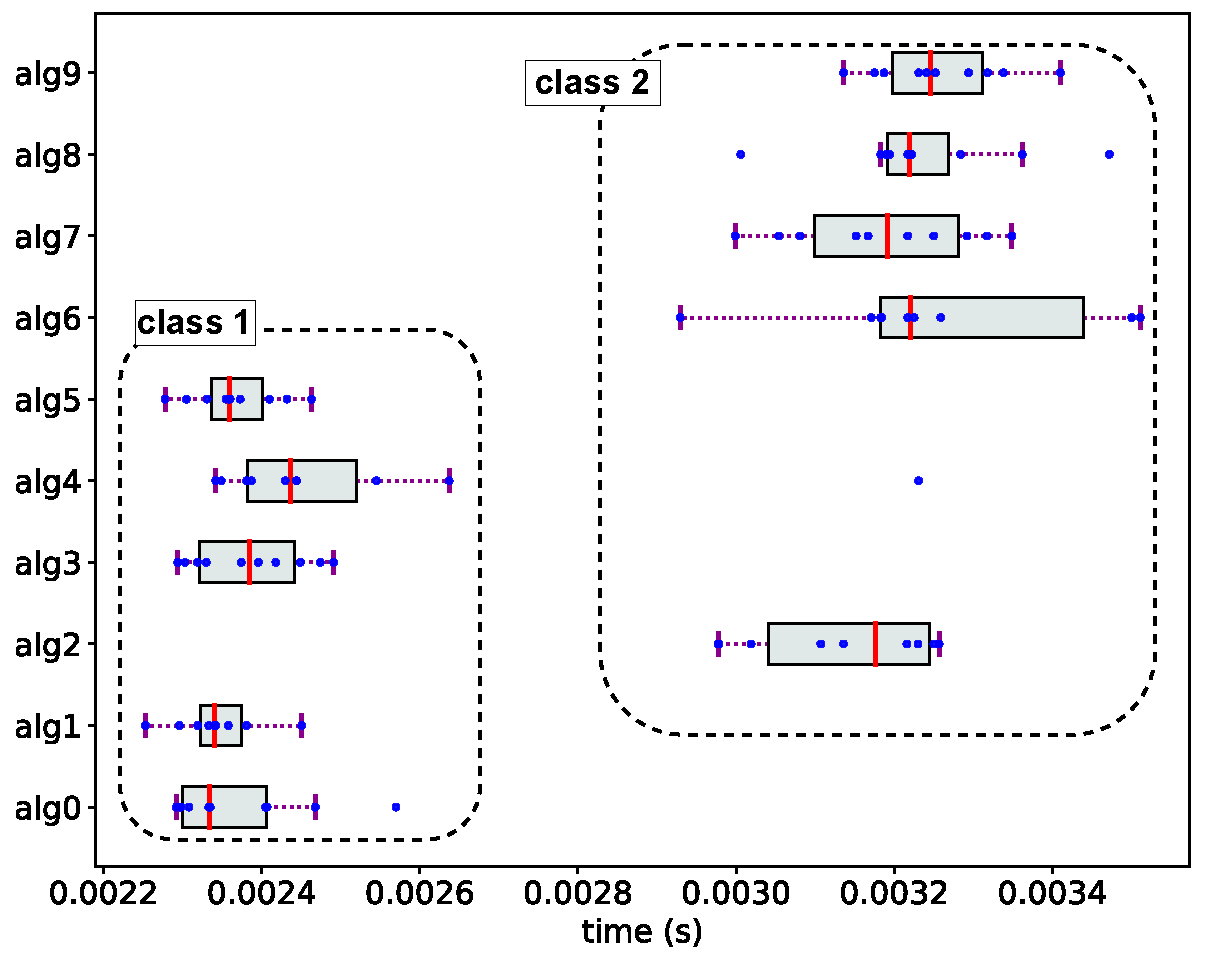
\includegraphics[width=0.6\linewidth]{fig/ch3/gls-eg-intro2}
	\caption{The execution time measurements of ten algorithmic variants to solve the GLS problem:  $(X^{T}M^{-1}X)^{-1}X^{T}M^{-1}\mathbf{y}$ where  $X \in \mathbb{R}^{1000 \times 100}$, $M \in \mathbb{R}^{1000 \times 1000}$ and $\mathbf{y} \in \mathbb{R}^{1000}$. For each variant, the execution times are shown as box plots; red lines indicate the median values; the box indicates the Inter-Quartile Interval. }
	\label{fig3:gls-eg-intro}
\end{figure}
Simple ranking approaches relying solely on summary statistics such as minimum or median values often lead to the assignment of a distinct rank to each variant, overlooking the ties (except when the statistics are exactly identical). By contrast, a ranking method that accounts for ties can group variants into \textit{performance classes}, where each class includes variants with the same rank. 
%Performance classes enable in highlighting the similarities and the differences in performance among the variants.  
Consider the two performance classes marked in Figure~\ref{fig3:gls-eg-intro} based on the following better-than relation ($<_{eg}$), which takes into account ties among the variants as follows:
\begin{enumerate}
	\item[$<_{eg}$ : ] A variant $\mathbf{alg}_i$ is considered to be better than another variant $\mathbf{alg}_j$ (i.e., $\mathbf{alg}_i <_{eg} \mathbf{alg}_j$) if and only if the IQI of $\mathbf{alg}_i$ lies entirely to the left of the IQI of $\mathbf{alg}_j$.  If the IQI of $\mathbf{alg}_i$ and $\mathbf{alg}_j$ overlap with one another, then  $\mathbf{alg}_i$ and $\mathbf{alg}_j$ are considered \textit{incomparable} (i.e., $\mathbf{alg}_i \sim \mathbf{alg}_j$).
\end{enumerate}
In typical ranking problems, it is assumed that the better-than relation follows a \textit{strict weak ordering} (i.e., not allowing for non-transitive ties). However, non-transitive ties can be expected in a noisy measurement data; in our example, $\mathbf{alg}_{1} \sim \mathbf{alg}_{3}$ and $\mathbf{alg}_{3} \sim \mathbf{alg}_{4}$, but $\mathbf{alg}_{1} <_{eg} \mathbf{alg}_{4}$. Therefore, the following ambiguity arises in the ranking process: should $\mathbf{alg}_{4}$ and $\mathbf{alg}_{1}$ be placed in different ranks because their intervals are separated, or show both be assigned the same rank because their intervals mutually overlap with that of $\mathbf{alg}_{3}$? 

% or not $\mathbf{alg}_{4}$ should be classified within class 1.  In this paper, we tackle such ambiguities by first defining what constitutes the set of reasonable rankings in general, and then develop methodologies to compute such rankings. Instead of a strict weak ordering, we approach the ranking problem based on better-than relations that follow \textit{strict partial ordering}, and therefore call the resulting rankings as \textit{partial rankings}. We then apply the methodology to the identification of the root cause of performance differences among the variants in different ranks in terms of library calls.


%The challenge in ranking sets of measurements that are infected by noise occurs especially when accounting for ties, as this introduces ambiguities to the ranking process. 
In general, it is possible to have several reasonable rankings for given sets of measurement data and a better-than relation. To illustrate how different rankings can be obtained through various arguments, let us utilize the following simulated example. Consider the set of objects or variants  $\mathcal{M} = \{\mathbf{t}_0, \mathbf{t}_1, \mathbf{t}_2, \mathbf{t}_3\}$ with each $\mathbf{t}_i \in \mathcal{M}$ indicated as a set of measurement values $\mathbf{t}_i\in \mathbb{R}^{M}$ sampled from normal distribution $\mathcal{N}(\mu, \sigma)$ that simulates the cost of the variant. Here, $\mu$ represents the mean and $\sigma$ represents the standard deviation of the normal distribution. Let us assume that the variants are characterized by the following distributions:
\begin{itemize}
	\setlength{\itemsep}{0pt} 
	\item $\mathbf{t}_0$: Sampled from $\mathcal{N}(0.30,0.005)$.
	\item $\mathbf{t}_1$: Sampled from $\mathcal{N}(0.31,0.030)$.
	\item $\mathbf{t}_2$: Sampled from $\mathcal{N}(0.32,0.005)$.
	\item $\mathbf{t}_3$: Sampled from $\mathcal{N}(0.43, 0.01)$.
\end{itemize}
For the purpose of sampling, we utilize a function from the NumPy library (version 1.22.0) in Python (version 3.9.7) to generate random normal values with the initialization seed set to 159. For each variant, $M=15$ values are sampled and the resulting set of values are depicted in Figure~\ref{fig3:intro-eg} as box plots.
 \begin{figure}[h!]
	\centering
	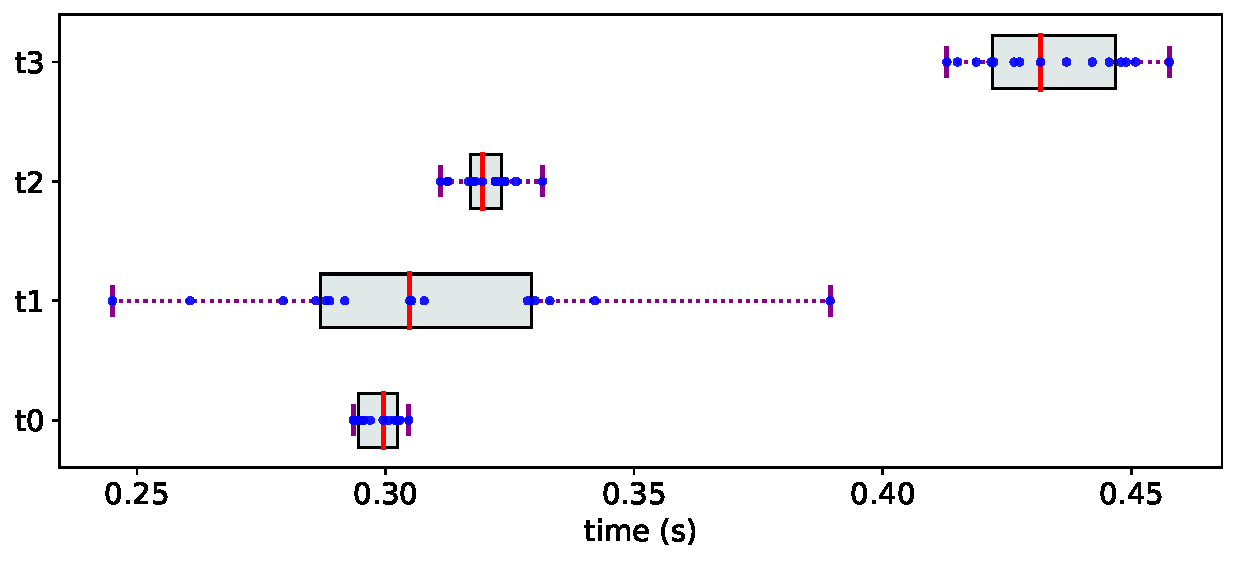
\includegraphics[width=0.6\linewidth]{fig/ch3/pr-def2-3}
	\caption{Sets of measurements ($\mathcal{M}_0$).}
	\label{fig3:intro-eg}
\end{figure}
%In order to compare two sets of measurements, let us consider the following better-than relation ($<_{eg}$), which takes into account ties among variants as follows:
%\begin{enumerate}
%	\item[$<_{eg}$ : ] A variant $\mathbf{t}_i$ is considered to be better than another variant $\mathbf{t}_j$ (i.e., $\mathbf{t}_i <_{eg} \mathbf{t}_j$) if and only if the IQI of $\mathbf{t}_i$ lies entirely to the left of the IQI of $\mathbf{t}_j$.  If the IQI of $\mathbf{t}_i$ and $\mathbf{t}_j$ overlap with one another, then  $\mathbf{t}_i$ and $\mathbf{t}_j$ are considered \textit{incomparable} (i.e., $\mathbf{t}_i \sim \mathbf{t}_j$).
%\end{enumerate}

For the sets of measurements ($\mathcal{M}_0$) in Figure~\ref{fig3:intro-eg}, the relation $<_{eg}$ among the variants is shown as a (transitively reduced) directed graph in Figure~\ref{fig:intro-dfgl}; a directed path from $\mathbf{t}_i$ to $\mathbf{t}_j$ indicates that $\mathbf{t}_i <_{eg} \mathbf{t}_j$. 
%According to $<_{eg}$, $\mathbf{t}_0 \sim \mathbf{t}_1$ and $\mathbf{t}_1 \sim \mathbf{t}_2$, but $\mathbf{t}_0  <_{eg} \mathbf{t}_2$; i.e., we see that the incomparability among the variants is not a transitive relation, and this leads to ambiguities in the ranking.
An example of the ambiguity for this case could be that the three rankings with ties shown in Figure~\ref{fig:intro-rank} are possible by the following justifications:

\begin{figure}[h!]
	\centering

	\begin{subfigure}[b]{0.48\textwidth}
		\centering
		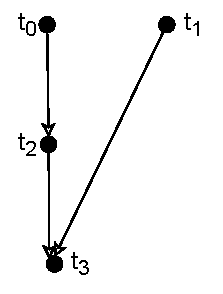
\includegraphics[width=0.3\linewidth]{fig/ch3/pr-def-partial.pdf}
		\caption{$<_{eg}$ on $\mathcal{M}_0$ shown as a transitively reduced directed graph.}
		\label{fig:intro-dfgl}
	\end{subfigure}
	\hfill
	\begin{subfigure}[b]{0.48\textwidth}
		%\centering
		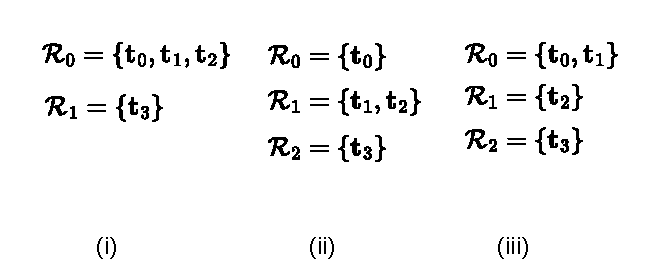
\includegraphics[width=0.8\linewidth]{fig/ch3/pr-def-rank-partial.pdf}
		\caption{Possible rankings deduced from Fig.~\ref{fig:intro-dfgl}. $\mathbf{t}_i \in \mathcal{R}_k$ implies $\mathbf{t}_i$ is assigned the rank $k$.}
		\label{fig:intro-rank}
	\end{subfigure}
	\caption{When distributions overlap, the partial ordering of the algorithms admits many reasonable rankings.}
	\label{fig:intro}
\end{figure}

\begin{itemize}
	\setlength\itemsep{0.1em}
	\item 
	One could argue that since $\mathbf{t}_0 \sim \mathbf{t}_1$ and $\mathbf{t}_1 \sim \mathbf{t}_2$, all $\mathbf{t}_0$, $\mathbf{t}_1$ and $\mathbf{t}_2$  should be given the same rank and considered as the best variants   (Fig~\ref{fig:intro-rank}(i)).
	
	\item Alternatively, one could argue that $\mathbf{t}_0$ should be ranked higher than $\mathbf{t}_2$ because $\mathbf{t}_0 <_{eg} \mathbf{t}_2$, and
	$\mathbf{t}_1$ should be ranked as low as $\mathbf{t}_2$ because the IQI of $\mathbf{t}_1$ overlaps with that of $\mathbf{t}_2$ (Fig~\ref{fig:intro-rank}(ii)). Then, only $\mathbf{t}_0$ should be considered as the best variant.
	
	\item Alternatively, since  $\mathbf{t}_0 \sim \mathbf{t}_1$ and $\mathbf{t}_0 <_{eg} \mathbf{t}_2$, one could argue that both $\mathbf{t}_0$ and $\mathbf{t}_1$ should be considered as the best variants, and $\mathbf{t}_2$ should be placed in a lower rank than $\mathbf{t}_0$  (Fig~\ref{fig:intro-rank}(iii)).
	 
%	\item $\mathbf{t}_0$ should be ranked higher than $\mathbf{t}_2$ because $\mathbf{t}_0 <_{eg} \mathbf{t}_2$, and $\mathbf{t}_1$ should be ranked as good as $\mathbf{t}_0$ because the IQI of $\mathbf{t}_1$ overlaps with that of $\mathbf{t}_0$ (Fig~\ref{fig:intro-rank}(iii)). Then, $\mathbf{t}_0$ and $\mathbf{t}_1$ are considered as the best variants. 
\end{itemize}

Thus, as soon as one considers a better-than relation that induces non-transitive ties, multiple reasonable rankings emerge. In this paper, we first define what constitutes the set of reasonable rankings in general, and then develop methodologies to compute such rankings. Instead of a strict weak ordering, we approach the ranking problem based on better-than relations that follow \textit{strict partial ordering}, and therefore call the resulting rankings as \textit{partial rankings}. We then apply the methodology to the identification of the root cause of performance differences among the objects.
%In this paper, we use many such simulated examples to explain our solutions to the partial ranking problem. 
%In this paper, we first define what constitutes the set of reasonable rankings in general, and then develop methodologies to compute such rankings. In typical ranking problems, it is assumed that the better-than relation follows a \textit{strict weak ordering} (i.e., not allowing for non-transitive ties). However, as non-transitive ties can be expected in a noisy measurement data, we tackle the ranking problem based on better-than relations that follow \textit{strict partial ordering}, and therefore call the resulting rankings as \textit{partial rankings}.  
  %We will see that the definition of what constitutes a set of reasonable rankings is important to develop and evaluate the correctness of the methodologies for ranking with ties, as straightforward approaches such as those applying Bubble-sort~\cite{sankaran2021performance, sankaran2022test} sometimes yield  rankings that are not generally considered reasonable, and this definition is required to detect and rectify those inaccuracies. 
The contributions of this work are the following:
\begin{enumerate}
	\setlength{\itemsep}{0pt} 
	%\item We illustrate the ambiguity issue related to ranking with ties based on noisy measurement data.
	
	\item  For given sets of measurements and a better-than relation that defines how two sets of  measurements should be compared, we define partial ranking to identify a set of reasonable rankings.
	
	\item We develop three different methodologies to compute some partial rankings for a given sets of measurements according to a given better-than relation.
	% First, we develop a directed graph-based methodology to compute a partial ranking that maximizes the number of ranks. Then, we develop a methodology to identify an alternative partial ranking with reduced number of ranks than what is computed using the directed-graph based approach. However, this methodology does not guarantee a partial ranking with minimum possible number of ranks. Finally, we develop another methodology to minimize the number of ranks. 
	
	%sort-based methodology, analyze the  adaptation of the Bubble-sort algorithm to identify a partial ranking and demonstrate that it does not always yield a valid partial ranking. However, even though this methodology  has limitations, they can still be employed to explore alternative partial rankings. Next, we employ a directed graph-based methodology to compute a partial ranking that maximizes the number of ranks. Then, we develop another methodology to reduce the number of ranks of a partial ranking  calculated using the directed graph-based approach. 
	
	\item We show that our partial ranking methodologies can be used to automatically discover the underlying causes of performance differences between the objects from the measurement data.
	 
	 %Specifically, we examine algorithmic variants of a Generalized Least Squares problem, and identify associations between library calls in the variants that lead to poor performance. We also consider the domain of Business Process Management and use our ranking methodology to perform root cause analysis on a widely utilized Purchase-to-Pay business process
	
	%\item  We demonstrate the application of partial ranking by using our methodologies on noisy performance measurements to discern observations that facilitate in identifying the causes of performance differences among the variants. Specifically, we examine algorithmic variants of a Generalized Least Squares problem, and identify associations between library calls in the variants that lead to poor performance. We also consider the domain of Business Process Management and use our ranking methodology to perform root cause analysis on a widely utilized Purchase-to-Pay business process.
\end{enumerate}


\paragraph{\textit{Organization: }} In Section~\ref{sec3:def}, we explain and formally define partial ranking. In Section~\ref{sec3:rel}, we discuss the related works. In Section~\ref{sec3:met}, we present methodologies for partial ranking of sets of measurements, and in Section~\ref{sec3:handlingq}, we extend our methodologies to handle multiple better-than relations. In Section~\ref{sec3:exp}, we apply the partial ranking methodology in two practical scenarios, and finally, in Section~\ref{sec3:con}, we draw conclusions.





\section{Partial Ranking}
\label{sec3:def}

Let $\mathcal{M} = \{\mathbf{t}_0, \dots, \mathbf{t}_{N-1}\}$ be a set of $N$ objects. Let $<_{\mathbf{P}} $ be a \textit{strict partial order} on $\mathcal{M}$ that models a better-than relation
%\footnote{Note that $<_{\mathbf{P}} $ is abstract; that is, a concrete procedure to compare two objects is not given. } 
between a pair of objects  $\mathbf{t}_i, \mathbf{t}_j \in \mathcal{M}$, i.e.,  $\mathbf{t}_i <_{\mathbf{P}}  \mathbf{t}_j$  means that $\mathbf{t}_i$ is somehow\textit{ better than} (e.g., faster than) $\mathbf{t}_j$. If  neither $\mathbf{t}_i <_{\mathbf{P}}  \mathbf{t}_j$ nor  $\mathbf{t}_j <_{\mathbf{P}}  \mathbf{t}_i$, then $\mathbf{t}_i$ and $\mathbf{t}_j$ are incomparable, which we denote by  $\mathbf{t}_i \sim \mathbf{t}_j$.
For each $\mathbf{t}_i \in \mathcal{M}$, we aim to assign a rank in the form of a non-negative integer with 0 representing the highest (best) rank that is consistent with $<_{\mathbf{P}} $. 
We first make a distinction between the cases where (1) we want the ranking to be unique and without ties, (2) we want the ranking to be unique but with ties, (3) the ranking cannot be unique but allows ties. 



\begin{enumerate}
	\setlength\itemsep{1em}
	\item \textbf{Linear order}  : If $\forall \mathbf{t}_i, \mathbf{t}_j \in \mathcal{M}$, either $\mathbf{t}_i <_{\mathbf{P}}  \mathbf{t}_j$ or  $\mathbf{t}_j <_{\mathbf{P}}  \mathbf{t}_i$, then $\mathcal{M}$ follows a \textit{linear order} for $<_{\mathbf{P}} $. In other words, $\nexists \mathbf{t}_i, \mathbf{t}_j \in \mathcal{M}$ such that $\mathbf{t}_i \sim \mathbf{t}_j$. In this case, we want the ranking to be unique and without ties.
	%\\
	
	\textit{Example:} Consider again the four sets of measurements $\mathcal{M}_0$ shown in  Figure~\ref{fig3:intro-eg} and the better-than relation $<_{med}$ where $\mathbf{t}_i <_{med} \mathbf{t}_j$ if and only if the median of $\mathbf{t}_i$ is smaller than the median of $\mathbf{t}_j$. According to $<_{med}$, the resulting ranking is the ordered set partition  ---$\mathcal{R}_0=\{\mathbf{t}_0\}$, $\mathcal{R}_1 = \{\mathbf{t}_1\}$, $\mathcal{R}_2 = \{\mathbf{t}_2\}, \mathcal{R}_3 = \{\mathbf{t}_3\}$--- of $\mathcal{M}_0$.
	 %Thus, commonly used median or mean-based rankings always induce a linear order but often ignore a significant amount of information that would suggest that a linear order is not reasonable.
	  Thus, $\mathcal{M}_0$ follows linear order for $<_{med}$.
	   %but not for $<_{eg}$. 
	   Consider another example $\mathcal{M}_1$ shown in Figure~\ref{fig:total-eg} and the better-than relation $<_{eg}$. 
	   %where linear order is indeed reasonable.
	   Here, $<_{eg}$ imposes linear order on $\mathcal{M}_{1}$, and the resulting ranking is shown in Figure~\ref{fig:total}(ii).
	
	
	\item \textbf{Weak order}: If $\forall \mathbf{t}_i, \mathbf{t}_j, \mathbf{t}_k \in \mathcal{M}$ such that $\mathbf{t}_i \sim \mathbf{t}_j$ and $\mathbf{t}_j \sim \mathbf{t}_k$, it holds $\mathbf{t}_i \sim \mathbf{t}_k$ (in  other words, the incomparability relation is transitive),  then $\mathcal{M}$ follows a \textit{weak order} for $<_{\mathbf{P}} $.   In this case,  we want the ranking to be unique, but this time with ties among all objects in the same equivalence class induced by the incomparability relation. 
	
	\textit{Example:} Consider the four sets of measurements $\mathcal{M}_2$ shown in Figure~\ref{fig:weak-eg} ordered by $<_{eg}$. The corresponding relations is shown in Figure~\ref{fig:weak}(i). The resulting ranking is illustrated in Figure~\ref{fig:weak}(ii). Here,  $\mathbf{t}_0, \mathbf{t}_1, \mathbf{t}_2 \in \mathcal{R}_0$ are all pairwise incomparable and all are assigned the same rank.
	
	\item \textbf{Neither linear nor weak}: If $\exists \mathbf{t}_i, \mathbf{t}_j, \mathbf{t}_k \in \mathcal{M}$ such that $\mathbf{t}_i \sim \mathbf{t}_j$, $\mathbf{t}_j \sim \mathbf{t}_k$ and $\mathbf{t}_i <_{\mathbf{P}} \mathbf{t}_k$ (in  other words, the incomparability relation is \textit{not} transitive), then $\mathcal{M}$ is neither linear nor weak for $<_{\mathbf{P}} $. In this case, the ranking will not be unique, for the reasons outlined in the introduction.

	
	\textit{Example}: The sets of measurements $\mathcal{M}_0$ in Figure~\ref{fig3:intro-eg} follows neither linear nor weak order for $<_{eg}$. For this case, we expect one of the three rankings shown in Figure~\ref{fig:intro-rank}. 
	%We would like to allow $\mathbf{t}_0$ and $\mathbf{t}_2$ to share the same rank despite $\mathbf{t}_0 <_{eg} \mathbf{t}_2$ because there exists an arrangement $\mathbf{t}_0 \sim \mathbf{t}_1 \sim \mathbf{t}_2$.

	%(or $\mathcal{M}$ is of type $\mathcal{M}_1$ ).  
\end{enumerate} 
\begin{figure}[h!]
	\centering
	\begin{subfigure}[b]{0.59\textwidth}
		\centering
		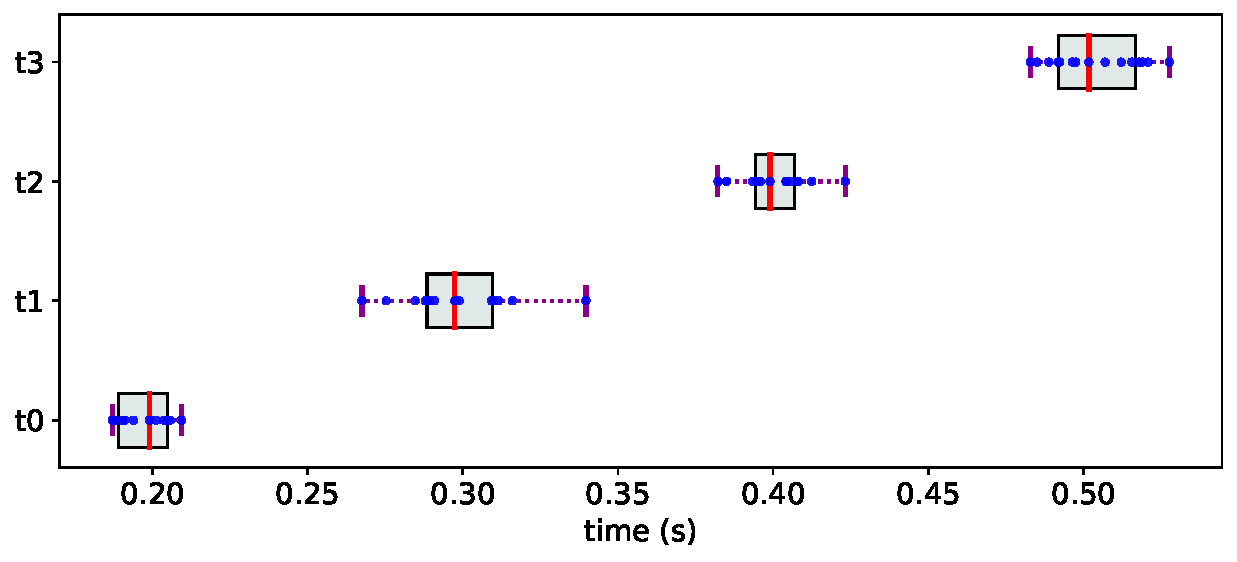
\includegraphics[width=1\linewidth]{fig/ch3/pr-def2-1}
		\caption{Sets of measurements $\mathcal{M}_1$.}
		\label{fig:total-eg}
	\end{subfigure}
	\begin{subfigure}[b]{0.39\textwidth}
		\centering
		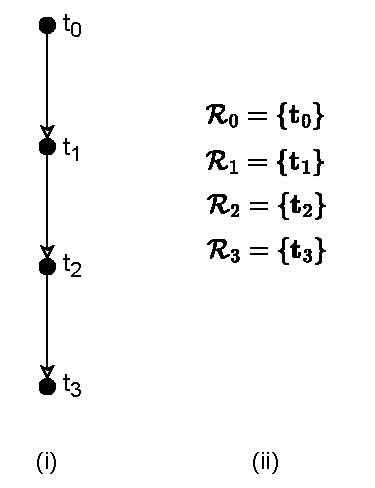
\includegraphics[width=0.6\linewidth]{fig/ch3/pr-def-total.pdf}
		\caption{$<_{eg}$ on $\mathcal{M}_1$ and the ranking (Linear order).}
		\label{fig:total}
	\end{subfigure}
	\par\bigskip
	\begin{subfigure}[b]{0.59\textwidth}
		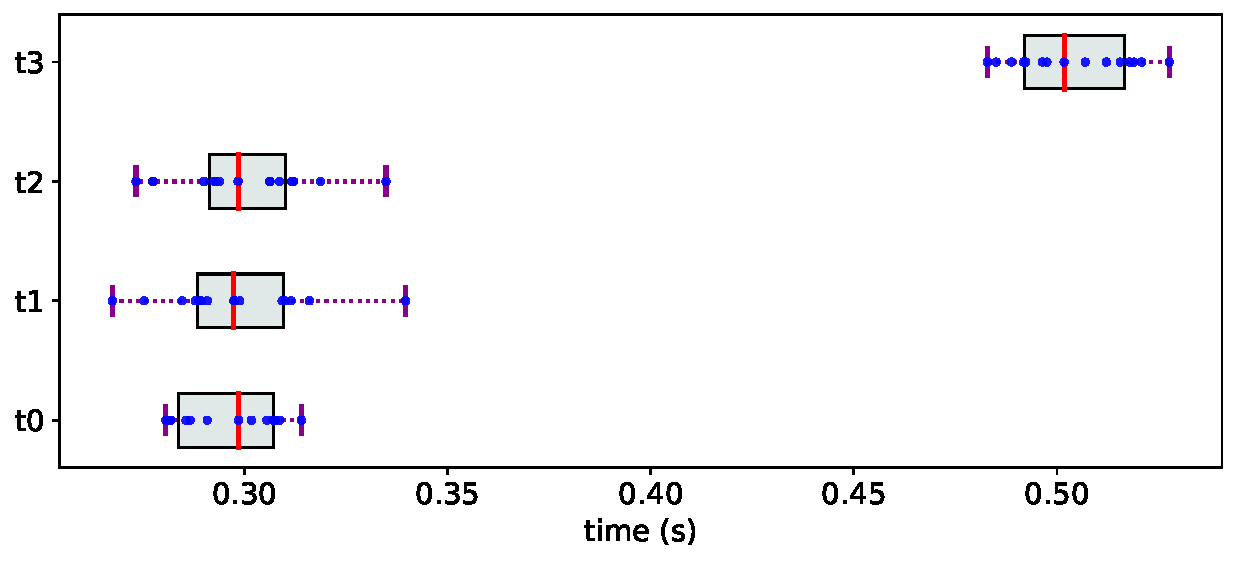
\includegraphics[width=1\linewidth]{fig/ch3/pr-def2-2}
		\caption{Sets of measurements $\mathcal{M}_2$.}
		\label{fig:weak-eg}
	\end{subfigure}
	\begin{subfigure}[b]{0.39\textwidth}
		\centering
		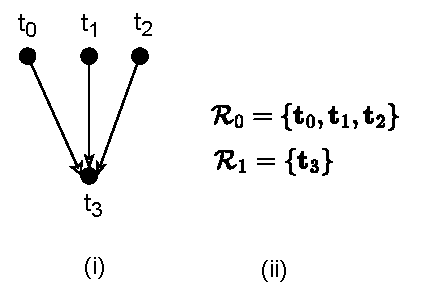
\includegraphics[width=0.85\linewidth]{fig/ch3/pr-def-weak.pdf}
		\caption{$<_{eg}$ on $\mathcal{M}_2$ and the ranking (Weak order).}
		\label{fig:weak}
	\end{subfigure}
	
	\caption{When $<_{\mathbf{P}} $ imposes either a linear order or a weak order on $\mathcal{M}$, then we want the ranking to be unique. Moreover, when the order is linear, then we want the ranking to have no ties.}
	\label{fig:pr-def}
\end{figure}

We now formulate a definition for ranking with ties that results in unique rankings when $<_{\mathbf{P}} $  imposes a linear or weak order on $\mathcal{M}$, and in more general cases allows only those rankings that satisfy the properties listed in the following.

%\clearpage

\begin{mydef}{Partial Ranking}{ranking}
	Given a set of objects $\mathcal{M}$ and a strict partial order relation $<_{\mathbf{P}} $ on $\mathcal{M}$, we define a \textit{partial ranking} as an ordered set partition $\mathcal{R}_0, \dots, \mathcal{R}_{K-1}$ of $\mathcal{M}$ with the following properties: 
	
	\begin{enumerate}
		\setlength\itemsep{0.5em}
		
		
		\item   If $\mathbf{t}_i$ is ranked higher than $\mathbf{t}_j$, then either $\mathbf{t}_i <_{\mathbf{P}}  \mathbf{t}_j$ or $\mathbf{t}_i \sim \mathbf{t}_j$.
		
		\item For all pairs of ranks $(\mathcal{R}_a, \mathcal{R}_b)$ where $b=a+1$, there exists a $\mathbf{t}_i \in \mathcal{R}_a$ and $\mathbf{t}_j \in \mathcal{R}_b$ such that $\mathbf{t}_i <_{\mathbf{P}}  \mathbf{t}_j$.  
		
		
		\item For all pairs $\mathbf{t}_i$ and $\mathbf{t}_j$ with the same rank, $\mathbf{t}_i$ and $\mathbf{t}_j$ must be connected in the undirected graph associated with the incomparability relation. 
		
		
		
	\end{enumerate}
\end{mydef}
\noindent The three properties serve the following purposes:
\begin{itemize}
	\item   Property~1 ensures that the ranking is consistent with the strict partial order.
	This property captures the essence of what we consider a reasonable ranking, since it prevents an object that is better than another from being ranked lower than the other.
	\item  Property~2 prohibits splitting up mutually incomparable objects into separate ranks. This property is essential to make the ranking unique for weak orders. For example, without this property, when $\mathcal{M}_2$ is ranked according to $<_{eg}$, the ranking $\mathcal{R}_0 = \{\mathbf{t}_0\}, \ \mathcal{R}_1 = \{\mathbf{t}_1, \mathbf{t}_2\}, \ \mathcal{R}_2 = \{\mathbf{t}_3\}$ would have been considered valid as it satisfies both Property 1 and Property 3. However, this ranking is not valid according to Property~2 because there does not exist a $ \mathbf{t}_i \in \mathcal{R}_0$ and $\mathbf{t}_j \in \mathcal{R}_1$ such that $\mathbf{t}_i <_{\mathbf{P}} \mathbf{t}_j$. 
	
	
	\item  Property~3 ensures that the objects with the same rank cannot be trivially partitioned into separate ranks. This property is essential for the uniqueness for both linear and weak orders, since without this property it would always be possible to assign all objects the same rank.  For example, without this property, for $\mathcal{M}_2$ and $<_{eg}$, the ranking $\mathcal{R}_0 = \{\mathbf{t}_0, \mathbf{t}_1, \mathbf{t}_2, \mathbf{t}_3\}$ would be considered valid as it satisfies both Property 1 and Property~2. However, according to Property~3, $\mathbf{t}_3$ cannot exist in the same rank as the other objects because $\mathbf{t}_3$ is disconnected in the undirected graph shown in Figure~\ref{fig3:undirected}.
\end{itemize}
%establishes the condition for valid ties. Notice that the Property~2 does not apply for linear orders (because  $\forall \mathcal{R}_a$, $|\mathcal{R}_a| = 1$). 
In summary, given $\mathcal{M}$ and $<_{\mathbf{P}}$, a ranking that satisfies the properties listed above is called a partial ranking. Now, the problem is to find a procedure that takes $\mathcal{M}$ as input, makes comparisons according to $<_{\mathbf{P}}$, and returns a partial ranking as output.

 \begin{figure}[h!]
	\centering
	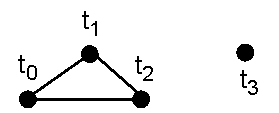
\includegraphics[width=0.2\linewidth]{fig/ch3/undirected}
	\caption{Undirected graph of the objects in $\mathcal{M}_2$ associated by $\sim$ according to $<_{eg}$.}
	\label{fig3:undirected}
\end{figure}




\section{Related Works}
\label{sec3:rel}

% \acc{TODO: a short para on ranking without ties; that is, ranking based on min or median. Here there are no ambiguities, but we cannot identify all the variants that could be considered the best.}



The problem of ranking with ties is generally seen as the partial ordering of a set of objects, in which the objects are related to one another based on a certain notion of importance~\cite{bruggemann2011ranking, janicki2008ranking}.
% whose ranks are determined based on certain notion that establishes the importance of one object over another~\cite{janicki2008ranking, Brüggemann2011-c2 }. 
%arranged based on their \textit{importance}\cite{janicki2008ranking}. Based on the notion that establishes the importance of one object over another,  a set of partially ordered pairs is constructed, from which a suitable ranking is determined~\cite{Brüggemann2011-c2}. 
%When there are more than one possible rankings, the structures in the partial order have been used to quantify the ambiguity in the ranking~\cite{Brüggemann2011-c5}. 
Although rankings based on partial orders have been widely discussed, we still notice a lack of clarity on what constitutes a reasonable ranking, especially when the partial order is neither linear nor weak. The term partial ranking has been previously used is some works (e.g.,~\cite{fagin2006comparing,ailon2010aggregation, pavan2004new}) to denote a ranking deduced from partial orders, but without much discussion of the properties of those rankings. In this work, we elaborate on partial ranking and explicitly list out its properties.

When it comes to methodologies for ranking based on partial orders, Pavan et al.~\cite{pavan2004new} explored the use of Hasse diagram technique to infer the ranks; i.e., a graph similar to the one shown in Fig~\ref{fig:intro-dfgl} is constructed, and the depth of a node in the graph is interpreted as the rank of that node. However, the ranking problem is addressed in the context of multi-attribute decision making, and the data is not considered as sets of measurements.  In~\cite{sankaran2022test, sankaran2021performance}, the Bubble-sort algorithm is used to develop a ranking methodology that allows for ties based on incomparable pairs of sets of measurements. However, the Bubble-sort based methodology is suited for a strict weak ordering and does not always compute a partial ranking. 
%In this work, we delve deeper into the Bubble-sort-based methodology and a Hasse-based methodology similar to~\cite{pavan2004new}, and demonstrate how they can be used to compute a partial ranking.

There is a large body of literature on the area of ranking, particularly tailored for applications in information retrieval; for example,  among the database community, \cite{ilyas2008survey} surveys the top-k ranking techniques for information retrieval and ~\cite{li2010ranking} discusses ranking approaches based on datasets that exhibit uncertainty. However, these works do not explicitly address the inherent ambiguities in rankings caused by noisy measurement data. Statistical ranking approaches such as~\cite{szekli1995stochastic} often require assumptions to be made regarding the underlying distribution of the measurement values, and the number of measurement values (or the sample size) plays an important role in determining whether or not the resulting rankings are meaningful.
%Moreover, when dealing with fluctuating measurements, the task of ranking them is commonly approached by summarizing the measurements using statistical measures such as mean, median~[?], or other relevant metrics, and the ties among the rankings are then accounted for by considering the overlap in the confidence intervals derived from those metrics [?]. Such approaches often require assumptions to be made regarding the underlying distribution of the measurement values, and the number of measurement values (or the sample size) plays an important role in determining whether or not the resulting rankings are meaningful.
 However, in many situations, measurements do not follow  standard distribution; for instance, the measurements of execution times in a compute system  are generally multi-modal (i.e., the measurement values occur in stratified clusters, mainly due to the processor operating at multiple frequency levels~\cite{charles2009evaluation}). As a result, it has been noted that the application of  textbook statistical approaches in summarizing such execution time measurements is not straightforward~\cite{chen2015statistical,hoefler2015scientific}. In this work, we consider the fact that the measurements could be noisy, but we do not make any assumption about their underlying distributions. Moreover, we focus on approaches that make use of the data---no matter how insufficient they are---as best as possible. 

%in the statistical approaches such as [?], 
%such as stochastic ordering~\cite{szekli2012stochastic},
%the number of measurement values (or the sample size) plays an important role in determining whether or not the resulting analyses are meaningful. By contrast, we focus on approaches that make use of the data---no matter how insufficient they are---as best as possible.
% For this reason, we avoid statistical approaches for ranking such as~\cite{szekli2012stochastic}, according to which execution times have to be considered as a random variable with a probabilistic interpretation. Instead, we consider execution times as an interval number between two quantiles. 
%Therefore, it is not straightforward to model the execution time of an algorithm as a random variable, approximate a probability distribution, and apply statistical approaches such as stochastic ordering~\cite{szekli2012stochastic} for ranking. In this paper, we consider the fact that a performance indicator could be noisy, but do not make any assumption about its underlying distribution, instead consider them as interval numbers; for instance, the execution time can be indicated as an interval between the 25th and 75th quantile of the measurements. 

In order to address the challenges posed by small sample sizes and the variability in measurement values, the spread of measurements is sometimes summarized using interval numbers~\cite{zhang2016ranking} or grey numbers~\cite{liu2014ranking}. While ranking approaches based on interval numbers have been applied in previous studies~\cite{liu2014ranking, ye2016method}, they have again focused mainly on the context of multi-attribute decision-making. In this paper,  we use the concept of interval numbers to compare two sets of measurements, but our focus is specifically on the ranking problem rather than decision-making. We clarify the ambiguities in the ranking by adopting our partial ranking definition. 

% In order to perform data comparisons despite small sample sizes, the spread of measurement values are sometimes summarized as interval numbers~\cite{ZHANG201662} or grey numbers~\cite{liu2014ranking}. Ranking approaches based on interval numbers have been applied in~\cite{liu2014ranking, ye2016method}, but mostly in the context of  multi-attribute decision making, without explicitly treating the  ambiguities in the rankings that arise due to noisy measurement data. In this work, instead of focusing on the decision making problem, we focus just on the ranking problem, and treat the ambiguites by approching the problem from the view point of partial ranking. 

%  (i.e., aggregating the ranks from more than one performance indicators to enable decision making). In this work, we focus on ambiguities in the ranking that arise even with the use of single attribute (e.g., just the execution times), and instead of trying to make a decision (such as choosing the best variant), we focus just on the ranking problem.


%\clearpage


\section{Methodologies For Partial Ranking}
\label{sec3:met}

 In this section, we develop methodologies to compute a partial ranking for a given $\mathcal{M}$ and $<_{\mathbf{P}}$. Let each $\mathbf{t}_i \in \mathcal{M}$ consist of $M_i$ measurement values (i.e.,  $\mathbf{t}_i \in \mathbb{R}^{M_i}$), and we assume that all $M_i \ge 1$. 


%\subsection{Methodology 1: Sort-based Partial Ranking}
%
%In order to be able to index the elements in the set $\mathcal{M}$, let us introduce a list $\mathbf{T}$. Initially, the elements in $\mathcal{M}$ are randomly arranged to form the list $\mathbf{T} = [\mathbf{t}_0, \dots, \mathbf{t}_{N-1}]$. The element at position $i$ (zero-based indexing) is denoted by $\mathbf{T}[i]$.
%%\footnote{We introduce the list $\mathbf{T}$ to be able to index the elements in the set $\mathcal{M}$.}.
%%The sort-based ranking methodology aims to solve the following problem:
%
%%\subsection{Formulations of the Partial Ranking Problem}
%\begin{mytheo}{\textit{Sort-based Partial Ranking}}{problemw}
%	Given $\mathbf{T}$ and the relation $<_{\mathbf{P}}$, the sort-based partial ranking consists of the following steps:
%	
%	
%	\begin{enumerate}
%		\item Sort $\mathbf{T}$ such that $\forall i<j$, either $\mathbf{T}[i] <_{\mathbf{P}} \mathbf{T}[j]$ or $\mathbf{T}[i] \sim \mathbf{T}[j]$.
%		%	\item  $ \forall \mathbf{T}[i] \in \mathbf{T}$, assign a rank $R[i]$ such that $R[0] = 0$,  $\mathbf{T}[i] <_p \mathbf{T}[i+1]$ implies $R[i+1] = R[i]+1$ and $\mathbf{T}[i] \sim \mathbf{T}[i+1]$ implies $R[i] = R[i+1]$.
%		%\item 
%		\item In the sorted $\mathbf{T}$, each $\mathbf{T}[i]$ is assigned  a rank $R[i]$  as follows: 
%		\begin{enumerate}
%			\item \textbf{set} $R[0] = 0$ (i.e., $\mathbf{T}[0]$ is assigned the best rank).
%			\item \textbf{for} \textit{i} = $1,\dots N-1$:
%			\begin{enumerate}
%				\item \textbf{if} $\mathbf{T}[i-1]  <_{\mathbf{P}} \mathbf{T}[i]$ \textbf{then} \textbf{set} $R[i] = R[i-1] +1$.
%				\item \textbf{else} \textbf{set} $R[i] = R[i-1]$.
%			\end{enumerate}
%		\end{enumerate}
%	\end{enumerate}
%\end{mytheo}
%%\noindent $R[i]$ is the rank of the variant at position $i$ in the sorted $\mathbf{T}$.
% \noindent According to Step~2b of Methodology~\ref{th:problemw}, adjacent variants in the sorted $\mathbf{T}$ that are incomparable to one another are assigned the same rank. Let $K$ be the number of unique values in $R$.
%The ordered set partition of $\mathcal{M}$ consists of sets within  which all the variants are assigned the  same rank; i.e.,
%\begin{equation}
%\label{eq:rank-sort}
%\mathcal{R}_k = \{ \mathbf{T}[i] \in \mathbf{T}\ | \  R[i] = k \} \qquad \forall k \in \{0, \dots, K-1\}
%\end{equation}
%and $\mathcal{R}_k$ consists of variants that receive the rank $k$.
%\begin{figure}[h!]
%	\centering
%	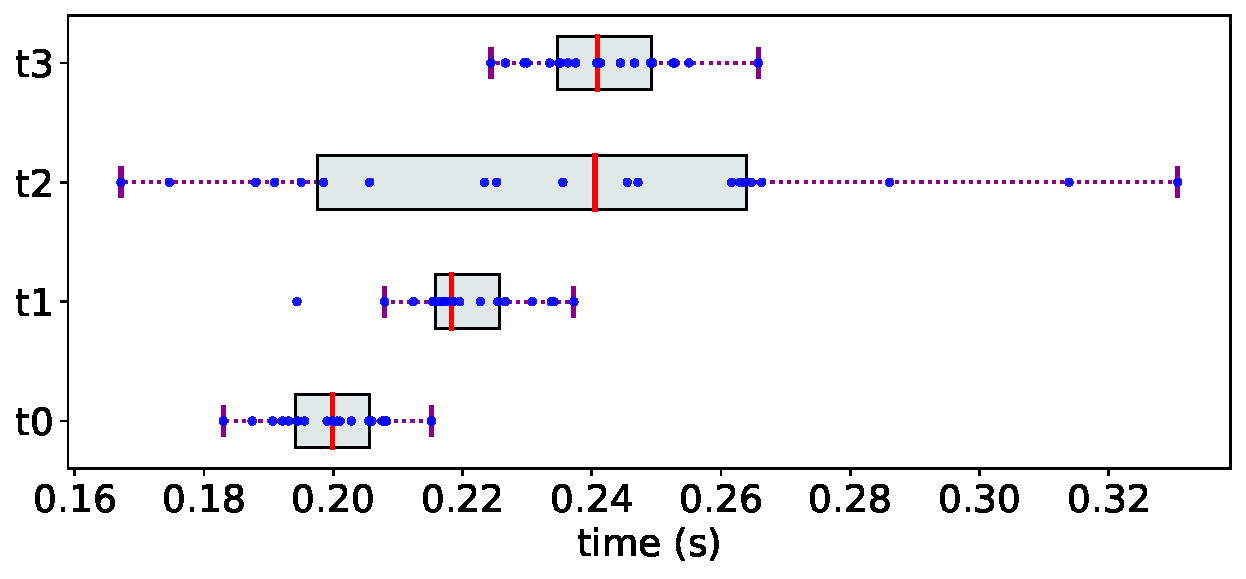
\includegraphics[width=0.6\linewidth]{fig/ch3/valid-3}
%	\caption{Sets of measurements $\mathcal{M}_4$. The box indicates the IQI.}
%	\label{fig3:met-eg}
%\end{figure}
%
%In general, for a given $\mathcal{M}$ and $<_{\mathbf{P}}$, there can be more than one possible sorted arrangement that are valid according to Methodology~\ref{th:problemw} (Step~1), and the rank assignments in Step~2 depend on the sorted arrangement.  For example, consider the sets of measurements $\mathcal{M}_4 = \{\mathbf{t}_0, \mathbf{t}_1, \mathbf{t}_2, \mathbf{t}_3\}$ shown in Figure~\ref{fig3:met-eg} and the relation $<_{eg}$. One possible sorted arrangement of $\mathcal{M}_4$ is $\mathbf{T} = [ \mathbf{t}_0, \mathbf{t}_3, \mathbf{t}_2, \mathbf{t} _1]$, and the corresponding array of ranks $R$ and the ordered set partitions $\mathcal{R}_k$ are shown in Table~\ref{tab3:met-ranks-eg}. Another possible sorted arrangement of $\mathcal{M}_4$ is $\mathbf{T} = [ \mathbf{t}_0, \mathbf{t}_1, \mathbf{t}_3, \mathbf{t} _2]$ for which the partial ranks are different from the one shown in Table~\ref{tab3:met-ranks-eg} and they are $\mathcal{R}_0 = \{\mathbf{t}_0\}$, $\mathcal{R}_1 = \{\mathbf{t}_1\}$, $\mathcal{R}_2 = \{\mathbf{t}_3, \mathbf{t}_2\}$.
%\begin{table}[h!]
%	\centering
%	\begin{adjustbox}{width=0.40\columnwidth,center}
%		\begin{tabular}{@{}ll cccccccc@{}}
%			\toprule
%			$\mathbf{T}$&& $\mathbf{T}$[0] &&$\mathbf{T}$[1] && $\mathbf{T}$[2] && $\mathbf{T}$[3]&\\
%			\cmidrule{3-10}
%			%\midrule
%			&& $\mathbf{t}_0$ &$<_{eg}$&  $\mathbf{t}_3$&$\sim$&  $\mathbf{t}_2$ &$\sim$ &  $\mathbf{t}_1$& \\
%			\midrule
%			$R$ &&$R$[0] &&$R$[1] && $R$[2] && $R$[3]&\\
%			\cmidrule{3-10}
%			&& 0 &&  1 &&  1 &&   1& \\
%			\midrule
%			$\mathcal{R}_k$&&\multicolumn{8}{c}{$\mathcal{R}_0 = \{ \mathbf{t}_0\}$, $\mathcal{R}_1 = \{\mathbf{t}_1, \mathbf{t}_2, \mathbf{t}_3\}$}\\
%			\bottomrule
%		\end{tabular}
%	\end{adjustbox}
%	\caption{A partial ranking of $\mathcal{M}_4$ with $<_{eg}$ according to Methodology~\ref{th:problemw}.}
%	\label{tab3:met-ranks-eg}
%\end{table}
%
%
%
%It is important to note that Step 1 of Methodology 1 requires a sorting process that goes beyond a simple arrangement where only adjacent elements $\mathbf{T}[i]$ and $\mathbf{T}[i+1]$ satisfy the condition $\mathbf{T}[i] <_p \mathbf{T}[i+1]$ or $\mathbf{T}[i] \sim \mathbf{T}[i+1]$. For instance, in Table~\ref{tab3:met-ranks-eg2}, we show an arrangement of $\mathcal{M}_4$ where, $\forall i$, $\mathbf{T}[i] <_p \mathbf{T}[i+1]$ or $\mathbf{T}[i] \sim \mathbf{T}[i+1]$, but the resulting ranking is not a partial ranking. In fact, there exists a non-adjacent pair of elements $ \mathbf{T}[0]=\mathbf{t}_1$ and $\mathbf{T}[3]=\mathbf{t}_0$ such that neither $\mathbf{T}[0] <_{eg} \mathbf{T}[3]$ nor $\mathbf{T}[0] \sim \mathbf{T}[3]$; as a consequence, $\mathbf{t}_0$ is ranked worse than $\mathbf{t}_1$ despite $\mathbf{t}_0 <_{eg} \mathbf{t}_1$. Hence, the sorted arrangement in Table~\ref{tab3:met-ranks-eg2} is not valid as it violates the condition in Step 1 of Methodology~\ref{th:problemw}.
%
%
%\begin{table}[h!]
%	\centering
%	\begin{adjustbox}{width=0.40\columnwidth,center}
%		\begin{tabular}{@{}ll cccccccc@{}}
%			\toprule
%			$\mathbf{T}$&& $\mathbf{T}$[0] &&$\mathbf{T}$[1] && $\mathbf{T}$[2] && $\mathbf{T}$[3]&\\
%			\cmidrule{3-10}
%			%\midrule
%			&& ${\color{red}\mathbf{t}_1}$ &$<_{eg}$&  $\mathbf{t}_3$&$\sim$&  $\mathbf{t}_2$ &$\sim$ &  ${\color{red}\mathbf{t}_0}$& \\
%			\midrule
%			$R$ &&$R$[0] &&$R$[1] && $R$[2] && $R$[3]&\\
%			\cmidrule{3-10}
%			&& 0 &&  1 &&  1 &&   1& \\
%			\midrule
%			$\mathcal{R}_k$&&\multicolumn{8}{c}{$\mathcal{R}_0 = \{$\acc{$\mathbf{t}_1$}$\}$, $\mathcal{R}_1 = \{$\acc{$\mathbf{t}_0$}$, \mathbf{t}_2, \mathbf{t}_3\}$}\\
%			\bottomrule
%		\end{tabular}
%	\end{adjustbox}
%	\caption{A ranking of $\mathcal{M}_4$ with $<_{eg}$ not valid according to Methodology~\ref{th:problemw}.}
%	\label{tab3:met-ranks-eg2}
%\end{table}
%
%\begin{mylem}{}{lemma1}
%	Rankings produced by Methodology~\ref{th:problemw} are partial rankings (Def.~\ref{th:ranking}).
%	%Equation~\ref{eq:rank-sort} is a valid partial ranking according to Definition~\ref{th:ranking}. 
%\end{mylem}
%\noindent \textit{Proof: } We need to prove that the ranking follows the three properties in Definition~\ref{th:ranking}.
%\begin{enumerate}
%	\item Proof for Property 1:
%	\begin{itemize}
%		\item $\forall \mathbf{T}[i] \in \mathcal{R}_a$ and  $\forall \mathbf{T}[j] \in \mathcal{R}_b$, $a<b \implies R[i] < R[j]$ (Eq.~\ref{eq:rank-sort}).
%		\item $R[i] < R[j] \implies i<j$  (Meth.~\ref{th:problemw}: Step 2b)
%		\item $i<j \implies \mathbf{T}[i] <_{\mathbf{P}} \mathbf{T}[j]$ or $\mathbf{T}[i] \sim \mathbf{T}[j]$ (Meth.~\ref{th:problemw}: Step 1).
%	\end{itemize}
%	Hence, $\forall \mathbf{T}[i] \in \mathcal{R}_a$ and  $\forall \mathbf{T}[j] \in \mathcal{R}_b$, $a<b \implies\mathbf{T}[i] <_{\mathbf{P}} \mathbf{T}[j]$ or $\mathbf{T}[i] \sim \mathbf{T}[j]$.
%	
%	\item Proof for Property 2: $\forall i, j$, $R[i] < R[j] \implies$  $\exists k \ge i$ and $l \le j$ such that $\mathbf{T}[k]  <_{\mathbf{P}} \mathbf{T}[l]$ (Meth.~\ref{th:problemw}: Step 2b).
%	
%	\item Proof for Property 3: $|\mathcal{R}_a| > 1 \implies $   $\exists k,l$ such that $\mathbf{T}[k] \sim \mathbf{T}[k+1] \sim \dots \sim  \mathbf{T}[l]$, and all the variants from positions $k$ to $l$ in the sorted $\mathbf{T}$ are  the only variants in $\mathcal{R}_a$ (Meth.~\ref{th:problemw}: Step 2). 
%	%	\begin{itemize}
%	%		\item $|\mathcal{R}_a| > 1$ implies there exists positions  $k$ and $m$ in the sorted $\mathbf{T}$ such that   $\mathbf{T}[k] \sim \mathbf{T}[k+1] \sim \dots \sim  \mathbf{T}[m]$ and all the objects from positions $k$ to $m$ in the sorted $\mathbf{T}$ are  the only objects in $\mathcal{R}_a$. 
%	%	\end{itemize}
%	Hence,  there exists an arrangement of $\mathcal{R}_a$ where the adjacent variants are pair-wise incomparable. 
%\end{enumerate}
%
%\textbf{Bubble Sort-based Ranking (BSR) Methodology:} 
%Let us analyse the use of the Bubble-sort algorithm~\cite{astrachan2003bubble} to form a sorted arrangement as required in Step 1 of Methodology~\ref{th:problemw}.
%Given $\mathbf{T}$ with some initial arrangement, Bubble-sort  is applied to sort $\mathbf{T}$ based on $<_{\mathbf{P}}$; i.e., starting from $\mathbf{T}[0]$, adjacent pairs of variants  are compared in sweeps according to the Bubble-sort algorithm,  and if a variant is better than the variant occurring immediately before it in the sequence, then they are swapped. In the sorted $\mathbf{T}$, the ranks of the variants are assigned as in Step 2 of Methodology~\ref{th:problemw}.  The sorted arrangement of the variants according to the Bubble-sort algorithm depends on the initial arrangement of the variants.
%
%
%
%\begin{table}[h!]
%	% 	\begin{minipage}{.5\linewidth}
%	% 		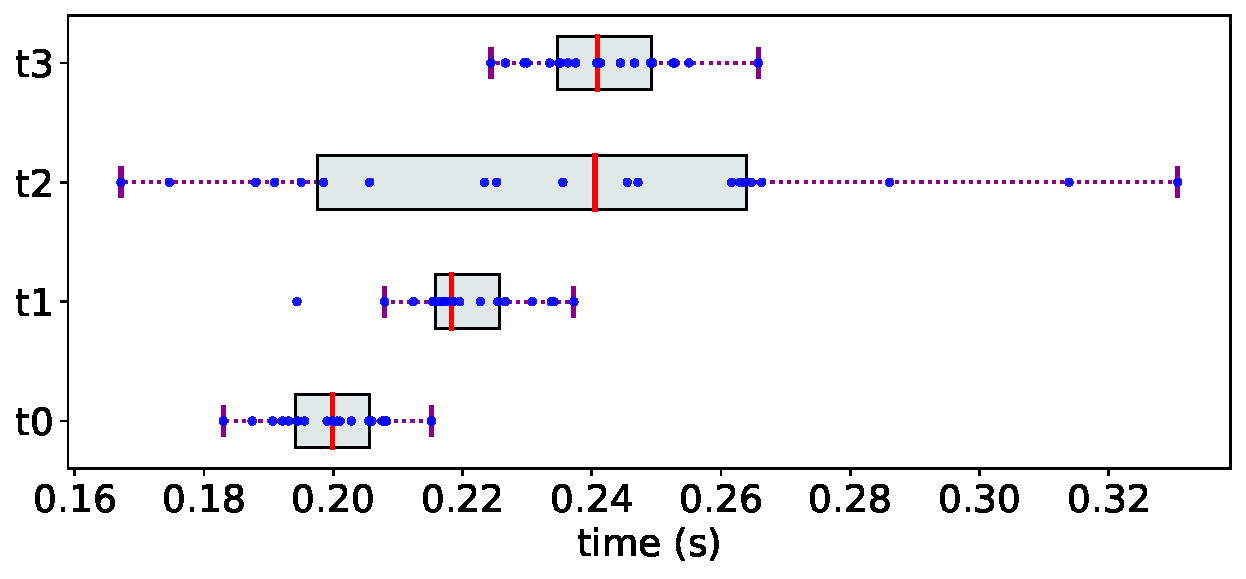
\includegraphics[width=1\linewidth]{fig/ch3/valid-3}
%	% 		\captionof{figure}{Example 1}
%	% 		\label{fig:met-eg}
%	% 	\end{minipage}
%	% 	\begin{minipage}{.5\linewidth}
%	% 		\centering
%	% 		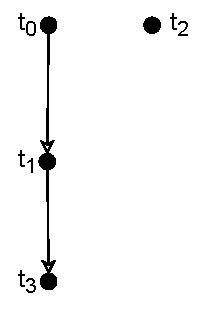
\includegraphics[width=0.45\linewidth]{fig/ch3/valid3-dfg}
%	% 		\captionof{figure}{$<_{eg}$ for Example 1}
%	% 		\label{fig:met-dfg}
%	% 	\end{minipage}%
%	% 	\bigskip
%	\centering
%	\renewcommand{\arraystretch}{1.0}
%	\begin{minipage}{0.7\linewidth}
%		\centering
%		\begin{adjustbox}{width=0.65\columnwidth,center}
%			\begin{tabular}{@{}ll cccccccc@{}}
%				\toprule
%				& & $\mathbf{T}_1$[0] &&$\mathbf{T}_1$[1] && $\mathbf{T}_1$[2] && $\mathbf{T}_1$[3]&\\
%				\midrule
%				(1)&& \acc{$\mathbf{t}_1$} &\acc{$>_{eg}$}&  \acc{$\mathbf{t}_0$}&? &  $\mathbf{t}_3$ &? &   $\mathbf{t}_2$& \\
%				%&$R$ && 0 &&  1 &&  2 &&   3& \\
%				%\midrule
%				(2)&& $\mathbf{t}_0$ &$<_{eg}$&  \ab{$\mathbf{t}_1$}&\ab{$<_{eg}$}&  \ab{$\mathbf{t}_3$} &? &   $\mathbf{t}_2$& \\
%				%&$R$ && 0 &&  1 &&  2 &&   3& \\
%				%\midrule
%				(3)&& $\mathbf{t}_0$ &$<_{eg}$&  $\mathbf{t}_1$&$<_{eg}$&  \ab{$\mathbf{t}_3$} & \ab{$\sim$} &   \ab{$\mathbf{t}_2$}& \\
%				%&\textit{R} && 0 &&  1 &&  2 &&   3& \\
%				%\midrule
%				(4)&& $\mathbf{t}_0$ &$<_{eg}$&  $\mathbf{t}_1$&$<_{eg}$&  $\mathbf{t}_3$ & $\sim$ &   $\mathbf{t}_2$& \\
%				\midrule
%				\textit{R} && 0 &&  1 &&  2 &&   2& \\
%				\midrule
%				\multicolumn{10}{c}{$\mathcal{R}_0 = \{\mathbf{t}_0\}$, $\mathcal{R}_1 = \{\mathbf{t}_1\}$, $\mathcal{R}_2 = \{\mathbf{t}_2, \mathbf{t}_3\}$}\\
%				\bottomrule
%			\end{tabular}
%		\end{adjustbox}
%		\caption{Valid Ranking with  $\mathbf{T}_1 =[\mathbf{t}_1, \mathbf{t}_0, \mathbf{t}_3, \mathbf{t}_2]$.}
%		\label{tab:met-ranks1}
%	\end{minipage} \\
%	\bigskip
%	\begin{minipage}{0.7\linewidth}
%		\centering
%		\begin{adjustbox}{width=0.65\columnwidth,center}
%			\begin{tabular}{@{}ll cccccccc@{}}
%				\toprule
%				&& $\mathbf{T}_2$[0] &&$\mathbf{T}_2$[1] && $\mathbf{T}_2$[2] && $\mathbf{T}_2$[3]&\\
%				\midrule
%				(1) && \ab{$\mathbf{t}_1$} &\ab{$<_{eg}$}&  \ab{$\mathbf{t}_3$}&? &  $\mathbf{t}_2$ &? &   $\mathbf{t}_0$& \\
%				%&$R$ && 0 &&  1 &&  2 &&   3& \\
%				%\midrule
%				(2)&& $\mathbf{t}_1$ &$<_{eg}$&  \ab{$\mathbf{t}_3$}&\ab{$\sim$}&  \ab{$\mathbf{t}_2$} &? &   $\mathbf{t}_0$& \\
%				%&$R$ && 0 &&  1 &&  2 &&   3& \\
%				%\midrule
%				(3) && $\mathbf{t}_1$ &$<_{eg}$&  $\mathbf{t}_3$&$\sim$&  \ab{$\mathbf{t}_2$} &\ab{$\sim$} &   \ab{$\mathbf{t}_0$}& \\
%				%&$R$ && 0 &&  1 &&  1 &&   2& \\
%				%\midrule
%				(4) && $\mathbf{t}_1$ &$<_{eg}$&  $\mathbf{t}_3$&$\sim$&  $\mathbf{t}_2$ &$\sim$ &  $\mathbf{t}_0$& \\
%				\midrule
%				$R$ && 0 &&  1 &&  1 &&   1& \\
%				\midrule
%				\multicolumn{10}{c}{$\mathcal{R}_0 = \{$\acc{$\mathbf{t}_1$}$\}$, $\mathcal{R}_1 = \{$\acc{$\mathbf{t}_0$}$, \mathbf{t}_2, \mathbf{t}_3\}$}\\
%				\bottomrule
%			\end{tabular}
%		\end{adjustbox}
%		\caption{Invalid Ranking with  $\mathbf{T}_2=[\mathbf{t}_1, \mathbf{t}_3, \mathbf{t}_2, \mathbf{t}_0]$.}
%		\label{tab:met-ranks2}
%	\end{minipage}
%\end{table}
%
%For example, consider the sets of measurements $\mathcal{M}_4$ and the relation $<_{eg}$. 
%%The objects are initially arranged according to increasing lengths of their IQnR
%Consider the two initial arrangements of $\mathcal{M}_4$,  $\mathbf{T}_1 = [\mathbf{t}_1, \mathbf{t}_0, \mathbf{t}_3, \mathbf{t}_2]$ and $\mathbf{T}_2 = [\mathbf{t}_1, \mathbf{t}_3, \mathbf{t}_2, \mathbf{t}_0]$. The steps of the Bubble-sort for $\mathbf{T}_1$ and $\mathbf{T}_2$ are shown in Table~\ref{tab:met-ranks1} and Table~\ref{tab:met-ranks2} respectively; in each step, a pair of adjacent variants are compared, and we omit showing the steps where two variants were already compared in a previous step. The pair of adjacent variants that are compared in a particular step are indicated in color; blue indicates that no swap in the positions is required, while red indicates a swap. A swap is indicated by the relation \acc{$\mathbf{t}_i >_{eg} \mathbf{t}_j$}, which is the same as $\mathbf{t}_j  <_{eg} \mathbf{t}_i$.  After the last step, the integer rank of each variant and the corresponding ordered set partition of $\mathcal{M}_4$ are shown.  We see that for input $\mathbf{T}_1$, the ranking is a partial ranking. However, for the input $\mathbf{T}_2$, the ranking is not a partial ranking because the rank of $\mathbf{t}_1$ is worse than that of $\mathbf{t}_0$ even though $\mathbf{t}_0 <_{eg} \mathbf{t}_1$, and this violates the requirement in Methodology~\ref{th:problemw} (Step 1), and consequently, the Definition~\ref{th:ranking} (Property 1).
%
%As the BSR methodology only compares adjacent pairs of elements to perform the swaps,  there is \textit{no} guarantee that the ranking computed according to this methodology is a partial ranking for \textit{all} initial arrangements.  Hence, the BSR methodology should include a validation step after the sorting to check if the condition according to Methodology~\ref{th:problemw} (Step~1) is met. If the condition is not met, then the BSR methodology should be repeated with an alternate initial arrangement. In the considered example, the problem occurred due to the placement of the object with the highest IQI range\footnote{IQI ranges are the length of the boxes in the box plots.}
%($\mathbf{t}_2$)  in between the first and the last object in the initial arrangement.  In order to reduce the occurrences of invalid results, we recommend an initial arrangement in which the members are arranged according to decreasing IQI lengths. 
%
%
%Thus, we showed that when a straightforward Bubble-sort based algorithm is used in the sorting step (i.e., Step~1) of Methodology~\ref{th:problemw}, a partial ranking is not guaranteed.  However, the BSR methodology along with a validation step can still be used to search for alternate partial rankings by changing the initial arrangement of the variants given as input. In the following sub-section, we develop a methodology that guarantees a partial ranking, but yields a unique solution and cannot be directly applied to search for alternative partial rankings. 

%but the partial ranking is unique and computes the partial ranking consisting of maximum number of ranks. 


\subsection{Methodology 1: For an arbitrary number of ranks}
\label{sec3:m2}

For a given $\mathcal{M}$ and $<_{\mathbf{P}}$, let $G$ be a directed graph such that $\mathbf{t}_i \in \mathcal{M}$ are the nodes, and a directed edge from $\mathbf{t}_i$ to $\mathbf{t}_j$ exists if and only if $\mathbf{t}_i <_{\mathbf{P}} \mathbf{t}_j$. A partial ranking can be computed from $G$ as follows:

\begin{mytheo}{\textit{Partial Ranking from a Directed Graph}}{problem2}
	Given the graph $G$ constructed from the partial order $(\mathcal{M}, <_{\mathbf{P}})$, set the rank of $\mathbf{t}_i \in \mathcal{M}$ equal to the length of the longest directed path in $G$ that ends at $\mathbf{t}_i$.
\end{mytheo}

Note that $G$ does not contain any cycles as $<_{\mathbf{p}}$ is transitive,
%\footnote{$\mathbf{t}_i <_{p} \mathbf{t}_j$ and $\mathbf{t}_j <_{p} \mathbf{t}_k$ automatically implies $\mathbf{t}_i <_{\mathbf{p}} \mathbf{t}_k$. This transitivity should not to be confused with non-transitivity of incomparability ($\sim$) among the variants.}
 and therefore, $G$ is a Directed Acyclic Graph. As a consequence,  the length of the longest directed path in $G$ that ends at $\mathbf{t}_i$ (or the \textit{depth} of $\mathbf{t}_i$ in $G$), denoted as $d(\mathbf{t}_i)$,  can be computed using the following recursive formula:
\begin{equation}
d(\mathbf{t}_i) = 
\begin{cases}
\underset{\mathbf{t}_j \in \bullet \mathbf{t}_i}{\max }  \ d(\mathbf{t}_j) + 1, & \text{if} \ |\bullet \mathbf{t}_i| > 0 \\
0, & \text{if}  \ |\bullet \mathbf{t}_i| = 0
\end{cases}
\end{equation}
where $\bullet \mathbf{t}_i$ is the set of incoming edges to $\mathbf{t}_i$. Then, the ordered set partition of $\mathcal{M}$ is:
\begin{equation}
\label{eq:rank-hesse}
\mathcal{R}_k = \{\mathbf{t}_i \in \mathcal{M}\ | \  d(\mathbf{t}_i) = k \} \qquad \forall k \in \{0, \dots, K-1\}
\end{equation}
where  $K-1$ is the length of the longest directed path in $G$. 

\begin{figure}[h!]
	\centering
	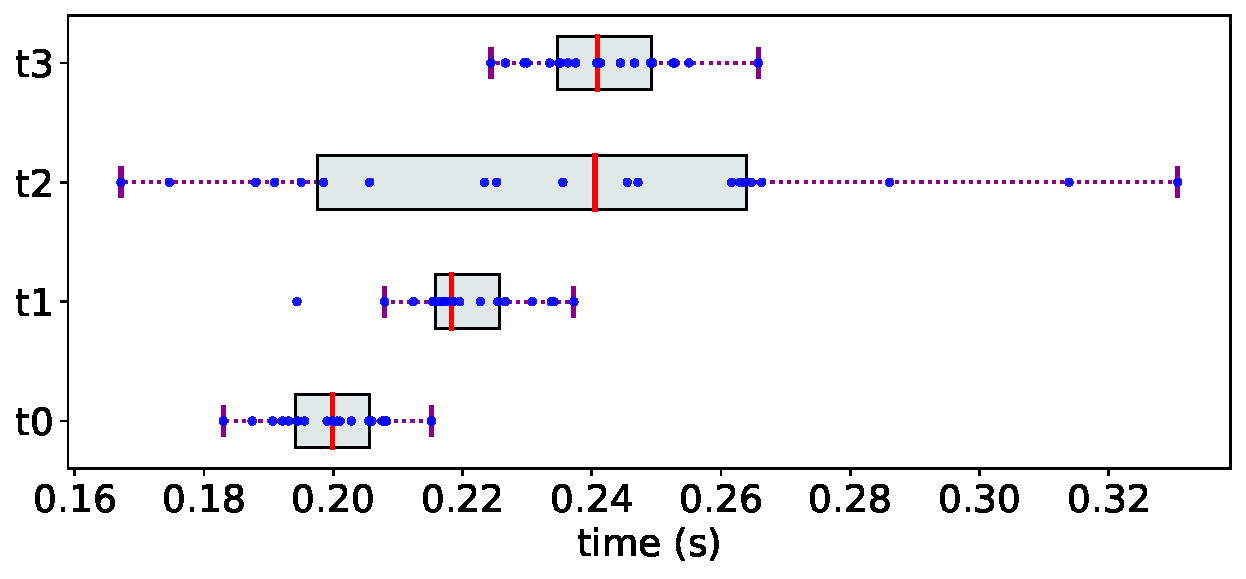
\includegraphics[width=0.6\linewidth]{fig/ch3/valid-3}
	\caption{Sets of measurements $\mathcal{M}_4$. The box indicates the IQI.}
	\label{fig3:met-eg}
\end{figure}

For example, consider the sets of measurements $\mathcal{M}_4$ in Figure~\ref{fig3:met-eg} and the relation $<_{eg}$. $\forall \mathbf{t}_i, \mathbf{t}_j \in \mathcal{M}_4$, we perform pair-wise comparison according to $<_{eg}$ and construct $G$ (shown in Figure~\ref{fig3:met-dfg}).  Note that performing transitivity reduction on a directed graph removes redundant edges without altering the depth of the nodes.  Consequently, it does not impact the ranking of the nodes. The transitive reduction of $G$ is shown in Figure~\ref{fig3:met-dfg-tr}. In both Figure~\ref{fig3:met-dfg} and Figure~\ref{fig3:met-dfg-tr},
the depth of $\mathbf{t}_0$ and $\mathbf{t}_2$ is 0, the depth of $\mathbf{t}_1$ is 1 and the depth of $\mathbf{t}_3$ is the maximum of $\{2,1\}$ which is 2. Hence, the ordered set partition is $\mathcal{R}_0 = \{\mathbf{t}_0, \mathbf{t}_2\}$, $\mathcal{R}_1 = \{ \mathbf{t}_1\}$, $\mathcal{R}_2 = \{\mathbf{t}_3\}$.

\begin{figure}[h!]
	\centering
	\begin{subfigure}{0.45\textwidth}
		\centering
		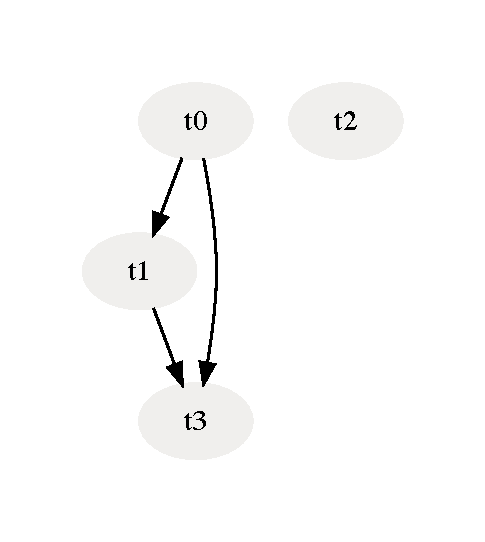
\includegraphics[width=0.7\textwidth]{fig/ch3/met-dfg}
		\caption{The graph $G$ associated with ($\mathcal{M}_4, <_{eg}$) }
		\label{fig3:met-dfg}
	\end{subfigure}
	\hfill
	\begin{subfigure}{0.42\textwidth}
		\centering
		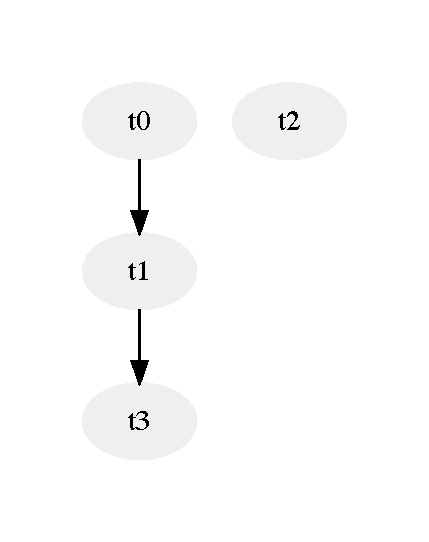
\includegraphics[width=0.7\textwidth]{fig/ch3/met-dfg-tr}
		\caption{Transitive reduction of $G$.}
		\label{fig3:met-dfg-tr}
	\end{subfigure}
	\caption{Directed graphs from the partial order ($\mathcal{M}_4, <_{eg}$)}
	\label{fig3:met-eg-g}
\end{figure}

\begin{mylem}{}{lemma2}
	Rankings produced by Methodology~\ref{th:problem2} are partial rankings (Def.~\ref{th:ranking}). 
	%and consists of maximum possible number of ranks.
\end{mylem}
\noindent \textit{Proof:} We need to prove that the ranking follows the three properties in Definition~\ref{th:ranking}.
\begin{enumerate}
	\item Proof for Property 1:
	\begin{itemize}
		\item  $\forall \mathbf{t}_i \in \mathcal{R}_a$ and  $\forall \mathbf{t}_j \in \mathcal{R}_b$, $a<b \implies  d(\mathbf{t}_i) < d(\mathbf{t}_j) $
		\item $d(\mathbf{t}_i) < d(\mathbf{t}_j) $ $\implies$ $\mathbf{t}_i <_{\mathbf{P}} \mathbf{t}_j$ or $\mathbf{t}_i \sim \mathbf{t}_j$.
	\end{itemize}
	
	\item Proof for Property 2: $\forall \mathcal{R}_a, \mathcal{R}_b$, $b=a+1 \implies$ there exists a directed edge from some $\mathbf{t}_i \in \mathcal{R}_a$ to some   $\mathbf{t}_j \in \mathcal{R}_b$, which means $\exists \mathbf{t}_i <_{\mathbf{P}} \mathbf{t}_j$.
	\item Proof for Property 3: Observe that in a directed acyclic graph, two nodes at the same depth cannot be connected by an edge, because if they were, then one of the nodes would be at a depth greater than the other node. Thus, $\forall \mathcal{R}_a$, $ \mathbf{t}_i, \mathbf{t}_j \in \mathcal{R}_a \implies $ $\mathbf{t}_i \sim \mathbf{t}_j$, so all the objects in $\mathcal{R}_a$ are connected in the undirected graph associated by $\sim$.
\end{enumerate}

%\begin{figure}[h!]
%	\centering
%	\begin{subfigure}{0.7\textwidth}
%		\centering
%		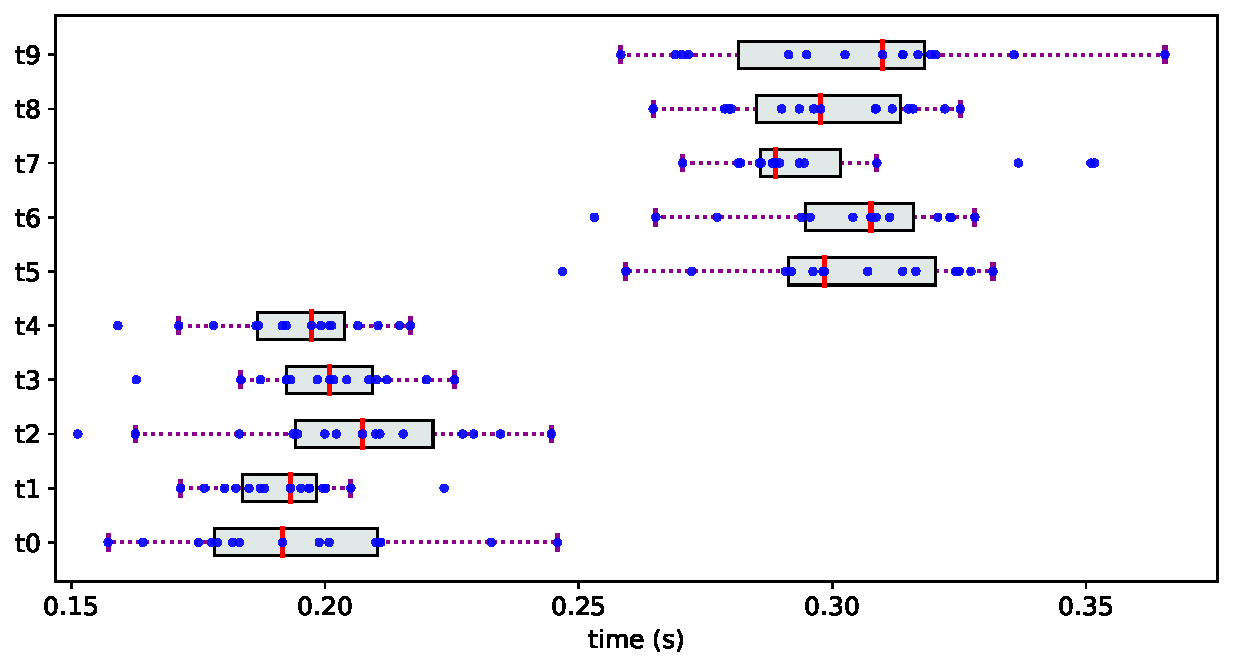
\includegraphics[width=\textwidth]{fig/ch3/hasse-eg-1}
%		\caption{Sets of measurements $\mathcal{M}_5$. }
%		\label{fig3:hasse-eg-1}
%	\end{subfigure}
%	\hfill
%	\begin{subfigure}{0.7\textwidth}
%		\centering
%		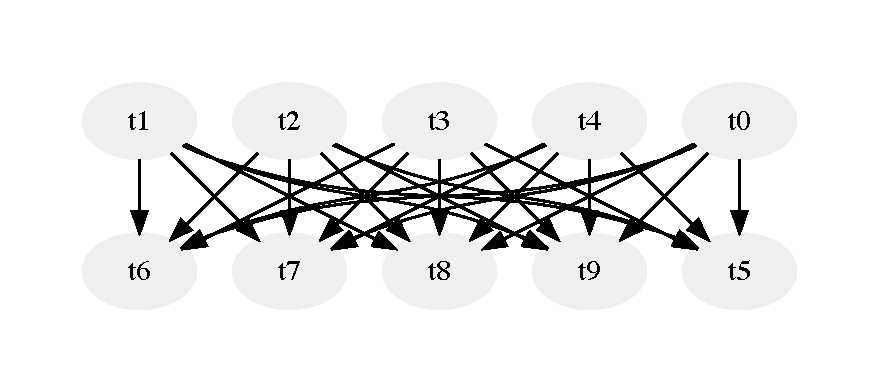
\includegraphics[width=0.8\textwidth]{fig/ch3/hasse-eg-1-dfg}
%		\caption{The graph $H$ associated with $\mathcal{M}_5$ and $<_{eg}$.\\$\mathcal{R}_0 = \{\mathbf{t}_0, \mathbf{t}_1, \mathbf{t}_2, \mathbf{t}_3, \mathbf{t}_4\}$, $\mathcal{R}_1 = \{\mathbf{t}_5, \mathbf{t}_6, \mathbf{t}_7, \mathbf{t}_8, \mathbf{t}_9\}$.}
%		\label{fig3:hasse-eg-1-dfg}
%	\end{subfigure}
%	\caption{An example where graph $H$ and $G$ are equivalent.}
%	\label{fig3:hasse-eg1}
%\end{figure}
\textbf{Sparsification of the directed graph:} Note that, in $G$, any directed edge from $\mathbf{t}_i$ to $\mathbf{t}_j$ such that $\mathbf{t}_i$ is at depth $k$ and $\mathbf{t}_j$ is at a depth greater than $k+1$ is not contained in the longest directed path to $\mathbf{t}_j$ in $G$.
Moreover, any modifications made to $G$ that do not impact the depths of its nodes have no influence on the calculated ranks according to Methodology~\ref{th:problem2}.
Bearing this in mind, we construct a graph $H$ from $G$ by removing all edges $(\mathbf{t}_i, \mathbf{t}_j)$ in $G$ where $d(\mathbf{t}_j) - d(\mathbf{t}_i) > 1$. The construction of $H$ ensures that the nodes at a specific depth are exclusively connected by directed edges only to nodes at the subsequent depth. 

% Bearing this in mind, we construct a graph $H$ such that the depths of the nodes in $H$ mirror those that would have been present in $G$. To this end, given $\mathcal{M}$ and $<_{\mathbf{P}}$, $\forall \mathbf{t}_i, \mathbf{t}_j \in \mathcal{M}$, perform pair-wise comparisons according to $<_{\mathbf{P}}$ and construct $H$ such that an edge $(\mathbf{t}_i, \mathbf{t}_j)$ exists if and only if the following two conditions are met:
%\begin{enumerate}
%	\item $\mathbf{t}_i <_{\mathbf{P}} \mathbf{t}_j$
%	\item $\nexists \mathbf{t}_k$ such that $\mathbf{t}_i \sim \mathbf{t}_k$ and a path exists from $\mathbf{t}_k$ to $\mathbf{t}_j$ consisting of at least two edges.
%\end{enumerate}

%The graph $H$ is a transitively reduced directed graph (also referred to as a directed Hasse graph),
 %The construction of $H$ ensures that the nodes at a specific depth are exclusively connected by directed edges only to nodes at the subsequent depth. 
%Note that any directed edge from $\mathbf{t}_i$ to $\mathbf{t}_j$ such that $\mathbf{t}_i$ is at depth $k$ and $\mathbf{t}_j$ is at a depth greater than $k+1$ is not contained in the longest directed path to $\mathbf{t}_j$. Therefore, the depth of $\mathbf{t}_j$ in $H$ remains the same as it would have been in $G$.
%As a consequence, for any node $\mathbf{t}_i \in H$, all its incoming nodes $\mathbf{t}_j \in \bullet \mathbf{t}_i$ share the same depth. Thus, the depth of a node $\mathbf{t}_i$ in $H$ is computed using a simplified recursive formula as follows:
%\begin{equation}
%\label{eq:depth2}
%d(\mathbf{t}_i, H) = 
%\begin{cases}
% d(\mathbf{t}_j, H) + 1, & \text{if} \ |\bullet \mathbf{t}_i| > 0 \\
%0, & \text{if}  \ |\bullet \mathbf{t}_i| = 0
%\end{cases}
%\end{equation}
%where $\mathbf{t}_j$ can be any one of the incoming nodes to $\mathbf{t}_i$.  The rankings can be computed by extracting the ordered set partition using Eq.~\ref{eq:rank-hesse}. 
%This methodology always produces a partial ranking with the maximum number of ranks.
\begin{figure}[h!]
	\centering
	\begin{subfigure}{0.7\textwidth}
		\centering
		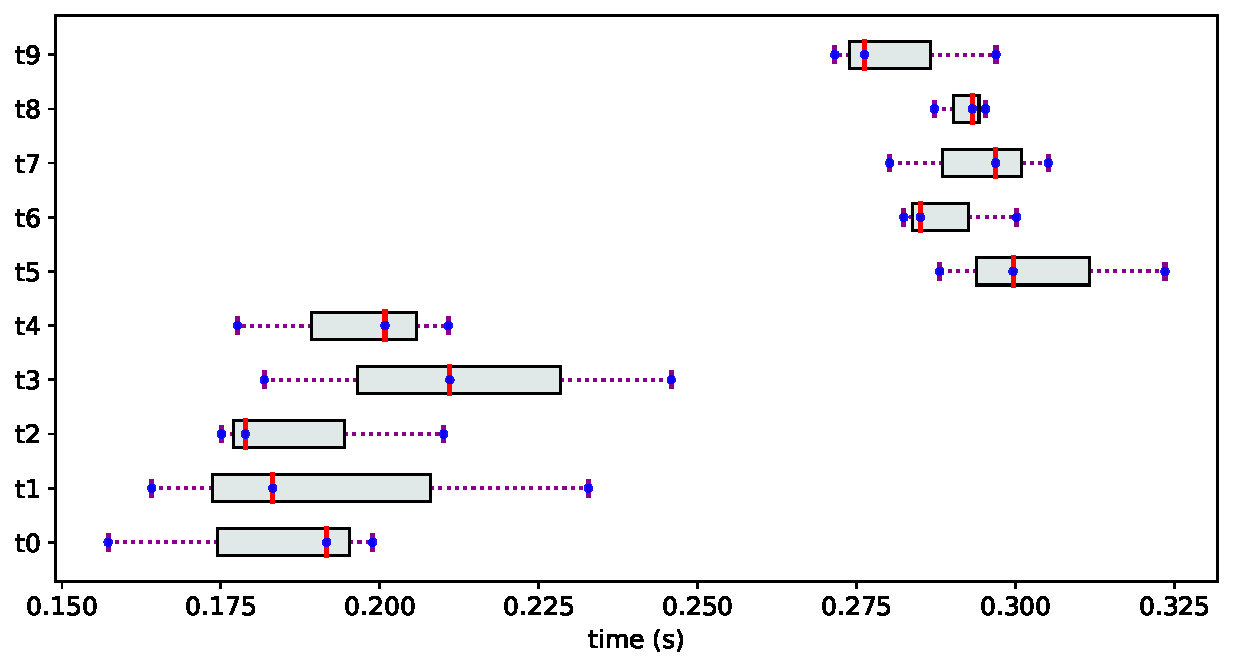
\includegraphics[width=\textwidth]{fig/ch3/hasse-eg-2}
		\caption{Sets of measurements $\mathcal{M}_6$. }
		\label{fig3:hasse-eg-2}
	\end{subfigure}
	\hfill
	\begin{subfigure}{0.5\textwidth}
		\centering
		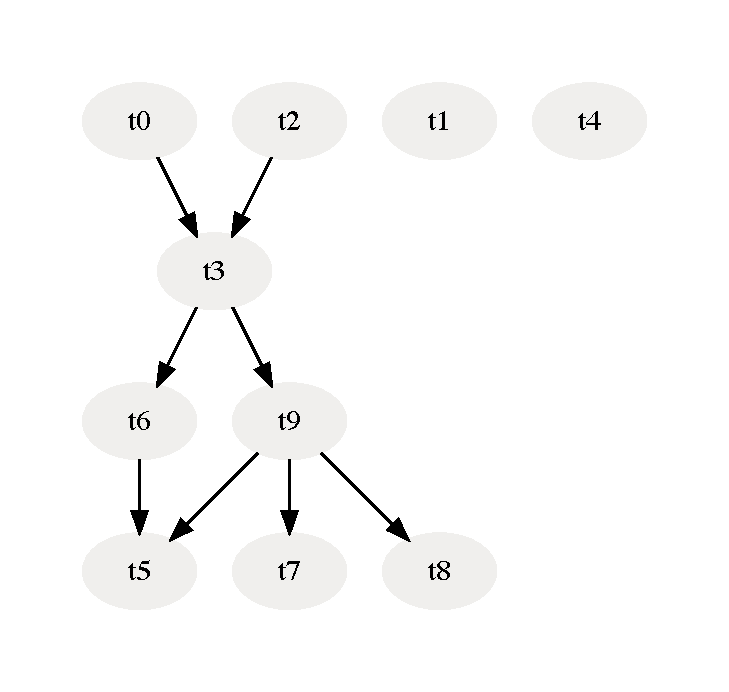
\includegraphics[width=\textwidth]{fig/ch3/hasse-eg-2-dfg}
		\caption{The graph $H$ associated with $\mathcal{M}_6$ and $<_{eg}$.\\$\mathcal{R}_0 = \{\mathbf{t}_0, \mathbf{t}_2, \mathbf{t}_1, \mathbf{t}_4\}$, $\mathcal{R}_1 = \{\mathbf{t}_3\}$, $\mathcal{R}_2 = \{\mathbf{t}_6, \mathbf{t}_9\}$, $\mathcal{R}_4 = \{\mathbf{t}_5, \mathbf{t}_7, \mathbf{t}_8\}$}
		\label{fig3:hasse-eg-2-dfg}
	\end{subfigure}
	\caption{An example to illustrate sparsification of $G$.  }
	\label{fig3:hasse-eg2}
\end{figure}

For example, consider the 10 variants consisting of measurements sampled from the following distribution functions :
\begin{itemize}
	\setlength{\itemsep}{0pt} 
	\item $\mathbf{t}_0, \mathbf{t}_1, \mathbf{t}_2, \mathbf{t}_3, \mathbf{t}_4 $: Sampled from $\mathcal{N}(0.2, 0.02)$
	\item $\mathbf{t}_5, \mathbf{t}_6, \mathbf{t}_7, \mathbf{t}_8, \mathbf{t}_9 $: Sampled from $\mathcal{N}(0.3, 0.02)$
\end{itemize}
For each variant, we sample 3 measurement values (with initialization seed set to 159) and prepare the sets of measurements $\mathcal{M}_6$ (shown in Figure~\ref{fig3:hasse-eg-2}). The partial rankings computed according to $<_{eg}$ are shown in Figure~\ref{fig3:hasse-eg-2-dfg}. Note that there is no path from $\mathbf{t}_4$ to $\mathbf{t}_9$ even though $\mathbf{t}_4 <_{eg} \mathbf{t}_9$ because the difference in the depths of $\mathbf{t}_4$ and $\mathbf{t}_9$ is 2.
Existence of the edge from $\mathbf{t}_4$ to $\mathbf{t}_9$ would not have changed the length of the longest directed path to $\mathbf{t}_9$.

%For each variant, we prepare two sets of measurement values with sample sizes $M=15$ and $M=3$ (with initialization seed set to 159), and the resulting measurement data are shown in Figure~\ref{fig3:hasse-eg-1} ($\mathcal{M}_5$) and Figure~\ref{fig3:hasse-eg-2} ($\mathcal{M}_6$) respectively. For $\mathcal{M}_5$ and $<_{eg}$, the graph $H$ and $G$ are equivalent, and hence no edges are removed. The resulting partial ranking consisting of two ranks are shown in Figure~\ref{fig3:hasse-eg-1-dfg}. For $\mathcal{M}_6$ and $<_{eg}$, the partial ranking, now consisting of four ranks, is shown in Figure~\ref{fig3:hasse-eg-2-dfg}. Here $H$ and $G$ are not equivalent. Note that in Figure~\ref{fig3:hasse-eg-2-dfg}, there is no path from $\mathbf{t}_4$ to $\mathbf{t}_9$ even though $\mathbf{t}_4 <_{eg} \mathbf{t}_9$. The edge from $\mathbf{t}_4$ to $\mathbf{t}_9$ is not present because there exists a path from $\mathbf{t}_2$ to $\mathbf{t}_9$ consisting of two edges. Existence of the edge from $\mathbf{t}_4$ to $\mathbf{t}_9$ would not have changed the length of the longest directed path to $\mathbf{t}_9$. 

%Even though both the measurement sets, $\mathcal{M}_5$ and $\mathcal{M}_6$, were sampled from the same distribution functions (\textbf{E1}), we observe that the Hasse-based methodology produces partial rankings having different number of ranks. However, it is important to note that even with the limited data $\mathcal{M}_6$, it is possible that alternative partial rankings exist, which may comprise a smaller number of ranks. 

%\clearpage

\subsection{Methodology 2: Reduction in the number of ranks}
 
We now explain how the partial ranking produced by Methodology~\ref{th:problem2} (sparsified) can be modified to determine an alternate partial ranking that might reduce the total number of ranks. 
Given the graph $H$ constructed from $\mathcal{M}$ and $<_{\mathbf{P}}$, the  ordered set partition $\mathcal{R}_0, \dots, \mathcal{R}_k, \dots, \mathcal{R}_{K-1}$ consisting of $K$ ranks (where $K$ is the length of the longest directed path in $H$) is computed using Eq.~\ref{eq:rank-hesse}. In order to determine if it is possible to produce an alternate partial ranking with smaller $K$, we apply the following methodology:

\begin{mytheo}{\textit{Rank reduction}}{problem3}
	%Given $\mathcal{M}$ and $<_{\mathbf{P}}$, perform the following steps:
	Given the graph $H$ and the corresponding ordered set partition $\mathcal{R}_0,\dots, \mathcal{R}_{K-1}$, perform the following steps:
	
	\begin{enumerate}
		%\item Construct the graph $H$ according to the Hasse-based methodology and determine the ordered set partition $\mathcal{R}_0, \dots, \mathcal{R}_k, \dots, \mathcal{R}_{K-1}$ consisting of $K$ ranks using Eq.~\ref{eq:rank-hesse}. 
		\item For all the nodes $\mathbf{t}_i$ in $H$, compute the number of incoming  and  outgoing edges.
		
		\item $\forall \mathcal{R}_k$, form a list\footnote{In order to be able to index the elements in the set $\mathcal{R}_k$, we introduce the list $\mathbf{R}_k$. The element at position $i$ (zero-based indexing) is denoted by $\mathbf{R}_k[i]$.} $\mathbf{R}_k$ by arranging the objects  in $\mathcal{R}_k$ according to decreasing number of outgoing edges in $H$. If there are objects with the same number of outgoing edges, arrange the objects with ties according to increasing number of incoming edges in $H$.
		
		\item Concatenate the lists into
		 %$\mathbf{T}$ by the concatenation ($\oplus$) of the lists $\forall\mathbf{R}_k$ from the highest to the lowest ranks; i.e.,  
		 $\mathbf{T} = \mathbf{R}_0 \oplus \mathbf{R}_1 \oplus \ldots \oplus \mathbf{R}_{K-1}$. Note that the objects in $\mathbf{T}$ are arranged left to right from highest to lowest ranks.
		
		\item  Each $\mathbf{T}[i]$ is assigned  a rank $R[i]$  as follows: 
				\begin{enumerate}
						\item \textbf{set} $R[0] = 0$ (i.e., $\mathbf{T}[0]$ is assigned the best rank).
						\item \textbf{for} \textit{i} = $1,\dots N-1$:
						\begin{enumerate}
								\item \textbf{if} $\mathbf{T}[i-1]  <_{\mathbf{P}} \mathbf{T}[i]$ \textbf{then} \textbf{set} $R[i] = R[i-1] +1$.
								\item \textbf{else} \textbf{set} $R[i] = R[i-1]$.
							\end{enumerate}
					\end{enumerate}
			%\end{enumerate}
%		\item Given $\mathbf{T}$, calculate the ranks according to Methodology~\ref{th:problemw} (Step~2) and extract the ordered set partition $\mathcal{\hat{R}}_0, \dots, \mathcal{\hat{R}}_{\hat{K}-1}$ using Eq.~\ref{eq:rank-sort} consisting of $\hat{K}$ ranks.
	\end{enumerate}
\end{mytheo}
\noindent According to Step~4b of Methodology~\ref{th:problem3}, adjacent objects in $\mathbf{T}$ that are incomparable to one another are assigned the same rank. Let $\hat{K}$ be the number of unique values in $R$.
The ordered set partition of $\mathcal{M}$ consists of sets within  which all the objects are assigned the  same rank; i.e.,
\begin{equation}
\label{eq:rank-sort}
\mathcal{\hat{R}}_k = \{ \mathbf{T}[i] \in \mathbf{T}\ | \  R[i] = k \} \qquad \forall k \in \{0, \dots, \hat{K}-1\}
\end{equation}
and $\mathcal{\hat{R}}_k$ consists of objects that receive the rank $k$. The new number of ranks $\hat{K}$ is smaller than or equal to $K$.

%In the step 2 of Methodology~\ref{th:problem3},  if $\exists \mathbf{t}_i \in \mathcal{R}_k$ and $\exists \mathbf{t}_j \in \mathcal{R}_{k+1}$ such that $\mathbf{t}_i \sim \mathbf{t}_j$, then $\mathbf{t}_i$ is pushed towards the right in the list $\mathbf{R}_k$, and $\mathbf{t}_j$ is pushed towards the left in the list $\mathbf{R}_{k+1}$, and then, the ranks $\forall \mathbf{t}_i \in \mathcal{R}_k$ and $\forall \mathbf{t}_j \in \mathcal{R}_{k+1}$ could be merged according to Methodology~\ref{th:problemw} (Step~2) with an input arrangement in which the elements of $\mathbf{R}_k$ are placed before the elements of $\mathbf{R}_{k+1}$.   Note that the construction of $\mathbf{T}$ in Methodology~\ref{th:problem3} (Step~3) ensures that the sorting condition according to  Methodology~\ref{th:problemw} (Step~1) is satisfied, because $\mathbf{R}_k$ is derived from $\mathcal{R}_k$ calculated according to the Hasse-based methodology, which implies $\forall \mathbf{t}_i, \mathbf{t}_j \in \mathbf{R}_k$, $\mathbf{t}_i \sim \mathbf{t}_j$ and $\forall a<b, \mathbf{t}_i \in \mathbf{R}_a, \mathbf{t}_j \in \mathbf{R}_b$ implies $\mathbf{t}_i \sim \mathbf{t}_j$ or $\mathbf{t}_i <_{\mathbf{P}} \mathbf{t}_j$. Hence the ranking $\mathcal{\hat{R}}_0, \dots, \mathcal{\hat{R}}_{\hat{K}-1}$ calculated in Methodology~\ref{th:problem3} is a partial ranking. 

\textbf{Illustrative Example}:  Consider the graph $H$ constructed from the sets of measurements $\mathcal{M}_6$ ranked according to $<_{eg}$  as shown in Figure~\ref{fig3:hasse-eg2}. The ordered set partition $\mathcal{R}_0, \mathcal{R}_1, \mathcal{R}_2, \mathcal{R}_3$ is shown in Figure~\ref{fig3:hasse-eg-2-dfg}. The arrangements according to Step~2 of Methodology~\ref{th:problem3} are:
\begin{itemize}
	\setlength{\itemsep}{0pt} 
	\item $\mathbf{R}_0 = [\mathbf{t}_0, \mathbf{t}_2, \mathbf{t}_1, \mathbf{t}_4]$
	\item $\mathbf{R}_1 = [\mathbf{t}_3]$
	\item $\mathbf{R}_2 = [\mathbf{t}_9, \mathbf{t}_6]$
	\item $\mathbf{R_3 = [\mathbf{t}_7, \mathbf{t}_8, \mathbf{t}_5]}$
\end{itemize}
The concatenated list according to Step~3 is:
\begin{equation}
\label{eq3:inp-arrange}
\mathbf{T} = [\mathbf{t}_0, \mathbf{t}_2, \mathbf{t}_1, \mathbf{t}_4, \mathbf{t}_3, \mathbf{t}_9, \mathbf{t}_6, \mathbf{t}_7, \mathbf{t}_8, \mathbf{t}_5]
\end{equation}
The ranking computed according to Methodology~\ref{th:problem3} with the list $\mathbf{T}$ in Eq.~\ref{eq3:inp-arrange} is shown in Table~\ref{tab3:min-ranks-eg1}, and consists of only two ranks.
\begin{table}[h!]
	\centering
	\begin{minipage}{\columnwidth}
		\centering
		\begin{adjustbox}{width=.9\columnwidth,center}
			\begin{tabular}{@{}ll cc cc cc cc cc cc cc cc cc cc@{}}
				\toprule
				$\mathbf{T}$&& $\mathbf{T}$[0] &&$\mathbf{T}$[1] && $\mathbf{T}$[2] && $\mathbf{T}$[3]&&$\mathbf{T}[4]$&&$\mathbf{T}[5]$&&$\mathbf{T}[6]$&&$\mathbf{T}[7]$&&$\mathbf{T}[8]$&&$\mathbf{T}[9]$&\\
				\cmidrule{3-22}
				%\midrule
				&& $\mathbf{t}_0$ &$\sim$&  $\mathbf{t}_2$&$\sim$&  $\mathbf{t}_1$ &$\sim$ &  $\mathbf{t}_4$&$\sim$&$\mathbf{t}_3$&$<_{eg}$&$\mathbf{t}_9$&$\sim$&$\mathbf{t}_6$&$\sim$&$\mathbf{t}_7$&$\sim$&$\mathbf{t}_8$&$\sim$&$\mathbf{t}_5$& \\
				\midrule
				$R$ &&$R$[0] &&$R$[1] && $R$[2] && $R$[3]&&$R$[4]&&$R$[5]&&$R$[6]&&$R$[7]&&$R$[8]&&$R$[9]&\\
				\cmidrule{3-22}
				&& 0 &&  0 &&  0 &&   0&&0&&1&&1&&1&&1&&1& \\
				\midrule
				$\mathcal{\hat{R}}_k$&&\multicolumn{20}{c}{$\mathcal{\hat{R}}_0 = \{ \mathbf{t}_0, \mathbf{t}_1, \mathbf{t}_2, \mathbf{t}_3, \mathbf{t}_4\}$, $\mathcal{\hat{R}}_1 = \{\mathbf{t}_5, \mathbf{t}_6, \mathbf{t}_7, \mathbf{t}_8, \mathbf{t}_9\}$}\\
				\bottomrule
			\end{tabular}
		\end{adjustbox}
		\caption{Partial ranking of $\mathcal{M}_6$ with $<_{eg}$ according to Methodology~\ref{th:problem3}.}
		\label{tab3:min-ranks-eg1}
	\end{minipage}
	\bigskip
	
	\begin{minipage}{.9\linewidth}
		\centering
		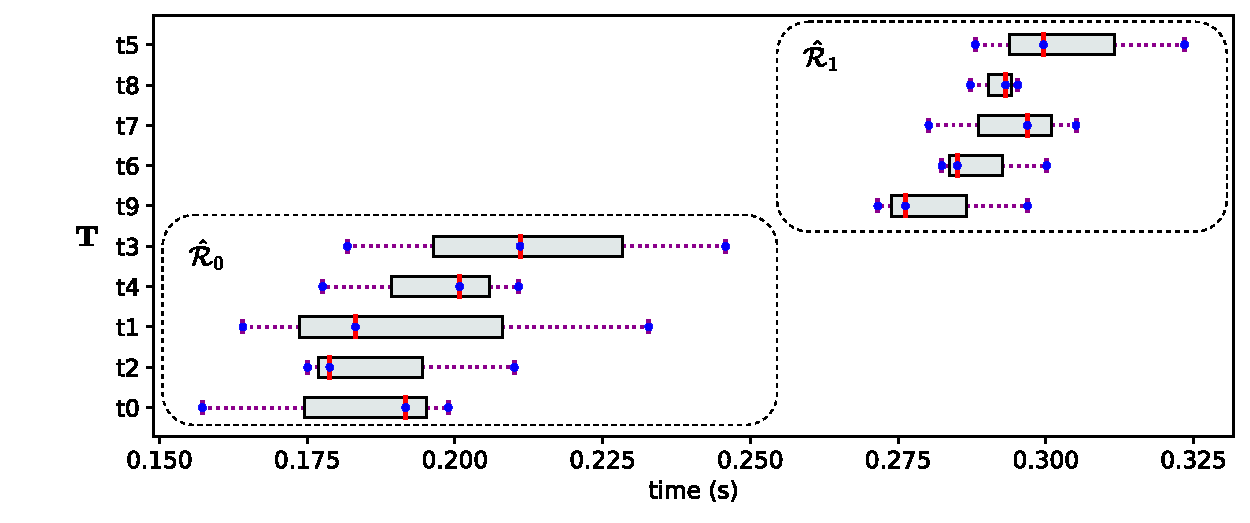
\includegraphics[width=0.9\textwidth]{fig/ch3/hasse-eg2-r}
		\captionof{figure}{The annotation of the partial ranking on $\mathcal{M}_6$  with $<_{eg}$ according to Methodology~\ref{th:problem3}. }
		\label{fig3:hasse-eg2-r}
	\end{minipage}
\end{table}

In the step 2 of Methodology~\ref{th:problem3},  if $\exists \mathbf{t}_i \in \mathcal{R}_k$ and $\exists \mathbf{t}_j \in \mathcal{R}_{k+1}$ such that $\mathbf{t}_i \sim \mathbf{t}_j$, then $\mathbf{t}_i$ is pushed towards the right in the list $\mathbf{R}_k$, and $\mathbf{t}_j$ is pushed towards the left in the list $\mathbf{R}_{k+1}$, and then, the ranks $\forall \mathbf{t}_i \in \mathcal{R}_k$ and $\forall \mathbf{t}_j \in \mathcal{R}_{k+1}$ could be merged according to Step~4. For illustration, 
let us denote the last element in a list $\mathbf{R}_k$ as $\mathbf{R}_k[-1]$. In our example, as $\mathbf{R}_0[-1] = \mathbf{t}_4 \sim \mathbf{t}_3 = \mathbf{R}_1[0] $,  the concatenation of $\mathbf{R}_0$ and $\mathbf{R}_1$ merges the ranks of the variants in $\mathcal{R}_0$ and $\mathcal{R}_1$. Similarly, as $\mathbf{R}_2[-1] = \mathbf{t}_6 \sim \mathbf{t}_7 = \mathbf{R}_3[0]$, the ranks of the variants in $\mathcal{R}_2$ and $\mathcal{R}_3$ are also merged. For the sake of clarity, the sets of measurements $\mathcal{M}_6$ are shown again in Figure~\ref{fig3:hasse-eg2-r}, but now with the y-axis re-arranged from bottom to top based on the position of the variants in the list $\mathbf{T}$, starting from $\mathbf{T}[0]$, and the ranking is annotated. 

\begin{mylem}{}{lemma1}
	Rankings produced by Methodology~\ref{th:problem3} are partial rankings (Def.~\ref{th:ranking}).
	%Equation~\ref{eq:rank-sort} is a valid partial ranking according to Definition~\ref{th:ranking}. 
\end{mylem}
\noindent \textit{Proof: } We need to prove that the ranking follows the three properties in Definition~\ref{th:ranking}.
\begin{enumerate}
	\item Proof for Property 1:
	\begin{itemize}
			\item $\forall \mathbf{T}[i] \in \mathcal{\hat{R}}_a$ and  $\forall \mathbf{T}[j] \in \mathcal{\hat{R}}_b$, $a<b \implies R[i] < R[j]$ (Eq.~\ref{eq:rank-sort}).
			\item $R[i] < R[j] \implies i<j$  (Meth.~\ref{th:problem3}: Step 4b)
			\item $i<j \implies \mathbf{T}[i] <_{\mathbf{P}} \mathbf{T}[j]$ or $\mathbf{T}[i] \sim \mathbf{T}[j]$ (Meth.~\ref{th:problem3}: Step 3; the objects in $\mathbf{T}$ are arranged from left to right from highest to lowest ranks computed according to Methodology~\ref{th:problem2}).
		\end{itemize}
	Hence, $\forall \mathbf{T}[i] \in \mathcal{\hat{R}}_a$ and  $\forall \mathbf{T}[j] \in \mathcal{\hat{R}}_b$, $a<b \implies\mathbf{T}[i] <_{\mathbf{P}} \mathbf{T}[j]$ or $\mathbf{T}[i] \sim \mathbf{T}[j]$.
	
	\item Proof for Property 2: According to Meth.~\ref{th:problem3}: Step 4b(i), a new rank is created only when there exists $i$ such that $\mathbf{T}[i-1]  <_{\mathbf{P}} \mathbf{T}[i]$. Hence, for every pair of ranks $\mathcal{\hat{R}}_a, \mathcal{\hat{R}}_b$, it is possible to find a pair $\mathbf{t}_i \in \mathcal{\hat{R}}_a$ and $\mathbf{t}_j \in \mathcal{\hat{R}}_b$ such that $\mathbf{t}_i <_{\mathbf{P}} \mathbf{t}_j$.   
	
	%$\forall i, j$, such that $R[i] < R[j] \implies$  $\exists k \ge i$ and $l \le j$ such that $\mathbf{T}[k]  <_{\mathbf{P}} \mathbf{T}[l]$ (Meth.~\ref{th:problem3}: Step 4b).
	
	\item Proof for Property 3: $|\mathcal{\hat{R}}_a| > 1 \implies $   $\exists k,l$ such that $\mathbf{T}[k] \sim \mathbf{T}[k+1] \sim \dots \sim  \mathbf{T}[l]$, and all the objects from positions $k$ to $l$ in $\mathbf{T}$ are  the only objects in $\mathcal{\hat{R}}_a$ (Meth.~\ref{th:problem3}: Step 4). 
	%	\begin{itemize}
		%		\item $|\mathcal{R}_a| > 1$ implies there exists positions  $k$ and $m$ in the sorted $\mathbf{T}$ such that   $\mathbf{T}[k] \sim \mathbf{T}[k+1] \sim \dots \sim  \mathbf{T}[m]$ and all the objects from positions $k$ to $m$ in the sorted $\mathbf{T}$ are  the only objects in $\mathcal{R}_a$. 
		%	\end{itemize}
	Hence,  there exists an arrangement of $\mathcal{\hat{R}}_a$ where the adjacent objects are pair-wise incomparable. This means that the objects in $\mathcal{\hat{R}}_a$ are connected in the undirected graph associated by $\sim$. 
\end{enumerate}

The number of ranks computed by Methodology~\ref{th:problem3} is either smaller than or equal to the number of ranks computed according to Methodology~\ref{th:problem2}, but not necessarily the least possible number of ranks.

\subsubsection{Instances where the least number of ranks is not computed}

\begin{figure}[h!]
	\centering
	\begin{subfigure}{0.85\textwidth}
		\centering
		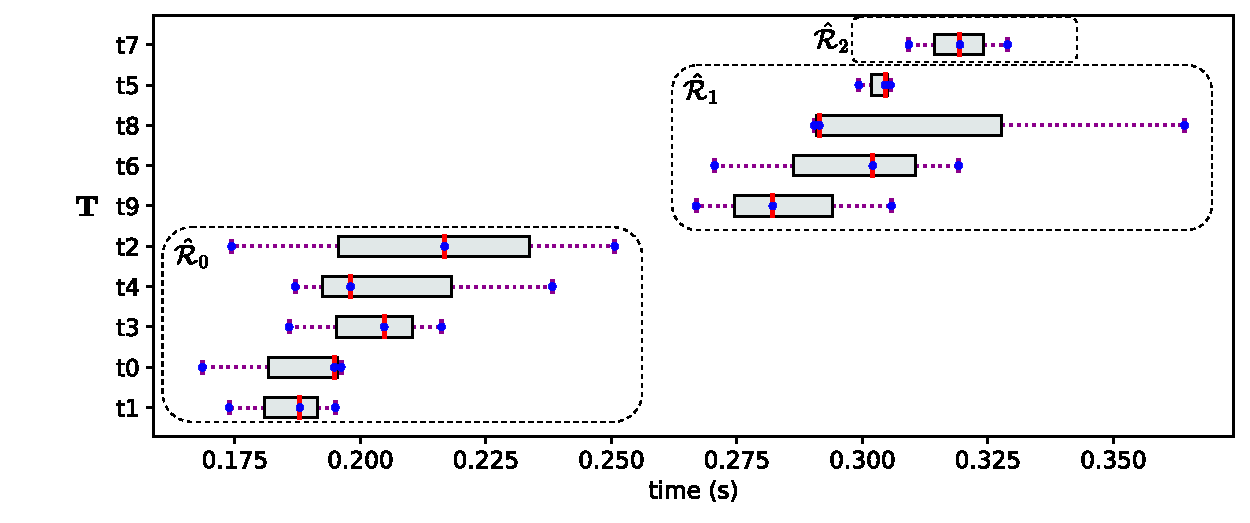
\includegraphics[width=0.8\textwidth]{fig/ch3/minrank-eg4-r}
		\caption{Methodology~\ref{th:problem3} on $\mathcal{M}_7$. }
		\label{fig3:minrank-eg4-r}
	\end{subfigure}
	\hfill
	\begin{subfigure}{0.85\textwidth}
		\centering
		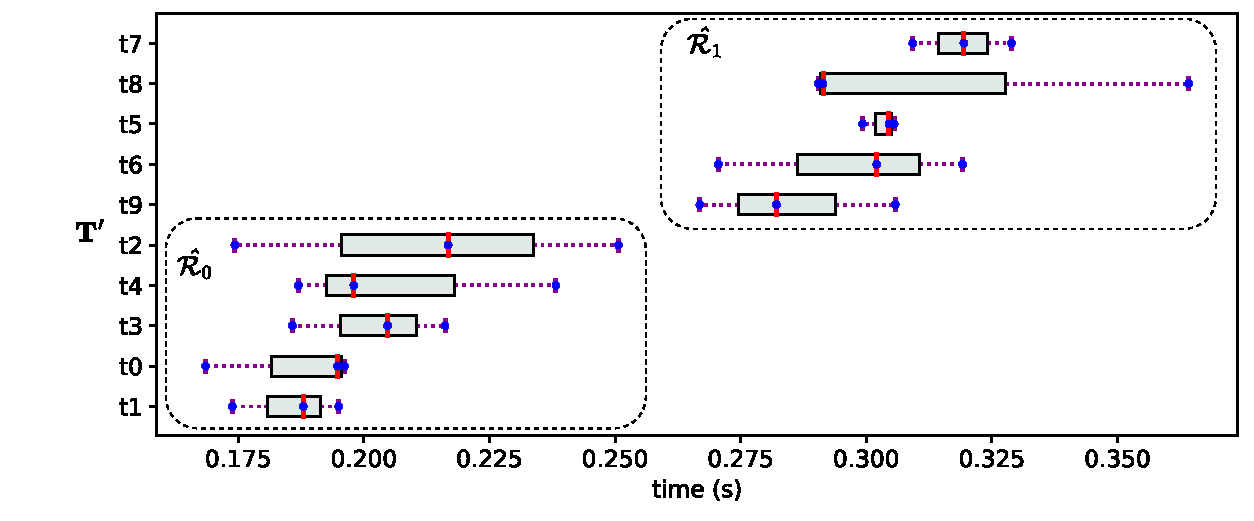
\includegraphics[width=0.8\textwidth]{fig/ch3/minrank-eg4-c}
		\caption{Methodology~\ref{th:problem3} on $\mathcal{M}_7$ with arrangement $\mathbf{T'}$.}
		\label{fig3:minrank-eg4-c}
	\end{subfigure}
	\hfill
	\begin{subfigure}{0.45\textwidth}
		\centering
		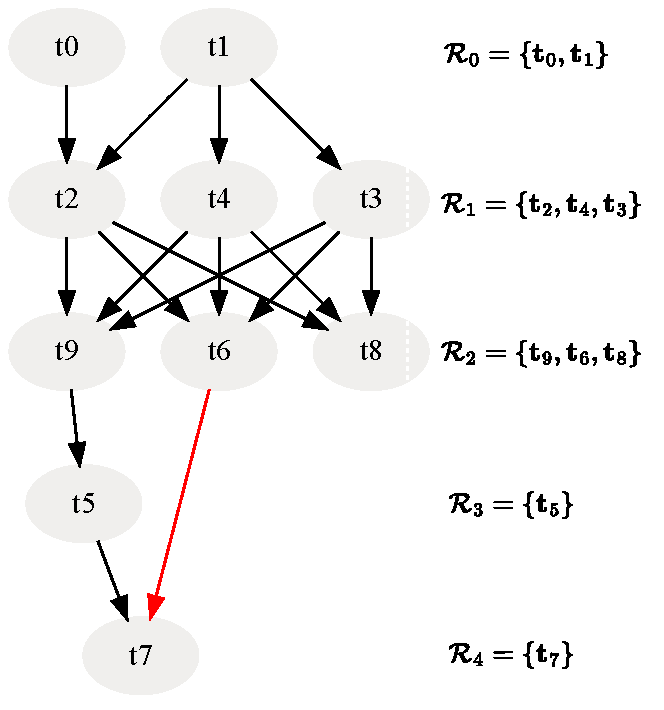
\includegraphics[width=0.8\textwidth]{fig/ch3/minrank-eg4-dfg}
		\caption{Methodology~\ref{th:problem2} on $\mathcal{M}_7$.  The transitivity reduction of graph $G$ for $\mathcal{M}_{7}$ according to $<_{eg}$. By removing the edge indicated in red, the graph $H$ is obtained.}
		\label{fig3:minrank-eg4-dfg}
	\end{subfigure}
	\caption{Partial ranking of $\mathcal{M}_{7}$ with $<_{eg}$. An illustrative example to demonstrate that Methodology~\ref{th:problem3} does not always find the partial ranking with the least number of ranks.  }
	\label{fig3:minrank-eg4}
\end{figure}

In certain cases, Methodology~\ref{th:problem3} does not yield a partial ranking with the minimum possible number of ranks. For example, consider the sets of measurements $\mathcal{M}_{7}$ shown in Figure~\ref{fig3:minrank-eg4}. Given $\mathcal{M}_{7}$ and $<_{eg}$, the arrangement $\mathbf{T}$ and the annotations of the partial ranking calculated according to Methodology~\ref{th:problem3} are shown in Figure~\ref{fig3:minrank-eg4-r}. While this partial ranking consists of three ranks, it is possible to form an alternate arrangement $\mathbf{T}'$ (shown in Figure~\ref{fig3:minrank-eg4-c}), that produces a partial ranking with just two ranks according to Methodology~\ref{th:problem3} (Step~4).
\begin{figure}[!h]
	\centering
	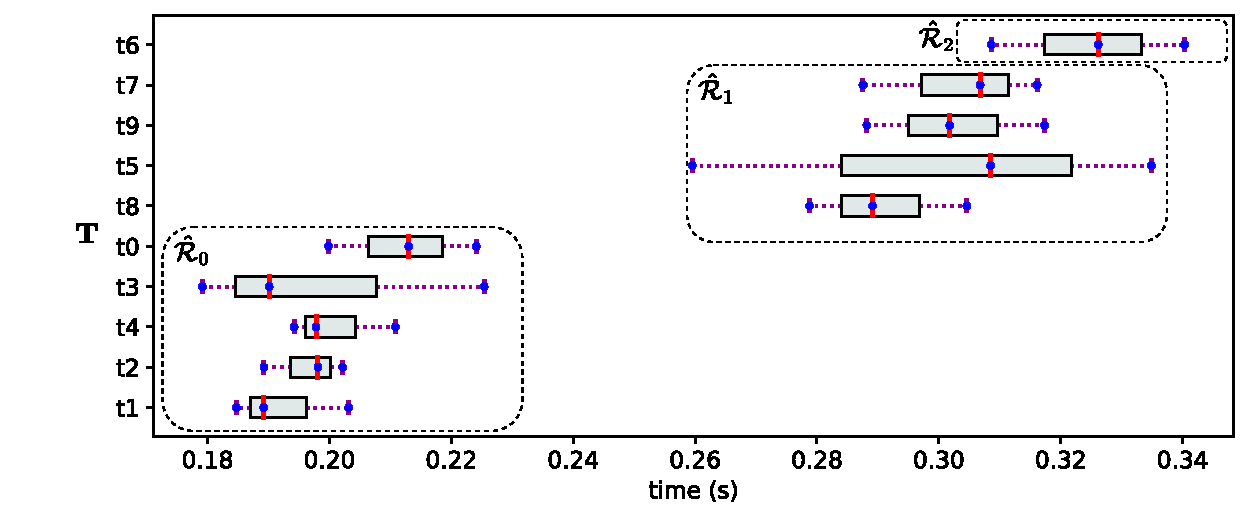
\includegraphics[width=0.8\textwidth]{fig/ch3/minrank-eg2-r}
	\caption{Partial ranking of $\mathcal{M}_8$ with $<_{eg}$ according to Methodology~\ref{th:problem3}.}
	\label{fig3:minrank-eg2-r}
\end{figure}

The following are some sufficient conditions for which Methodology~\ref{th:problem3} will not produce a partial ranking with the least number of ranks:
\begin{enumerate}
	\item $\exists \mathbf{t}_i \in \mathcal{R}_k$ and $\exists \mathbf{t}_j \in \mathcal{R}_{k+2}$ such that $\mathbf{t}_i \sim \mathbf{t}_j$, but $\nexists \mathbf{t}_m \in \mathcal{R}_{k+1}$ such that $\mathbf{t}_m \sim \mathbf{t}_j$.
	\item  $\exists \mathbf{t}_i <_{P} \mathbf{t}_j$ and $\mathbf{t}_j <_{P} \mathbf{t}_k$, but all $\mathbf{t}_i, \mathbf{t}_j, \mathbf{t}_k$ are associated by $\sim$ to another variant $\mathbf{t}_l$. 
\end{enumerate}

\textit{Example for condition~1}: For $\mathcal{M}_7$, the directed graph $G$ (with transitivity reduction) is shown in Figure~\ref{fig3:minrank-eg4-dfg} (by removing the edge highlighted in red, the graph $H$ is obtained). According to Methodology~\ref{th:problem2}, the number of ranks is 5, and we just saw that it possible to have a partial ranking consisting of 2 ranks. Methodology~\ref{th:problem3} cannot reduce the number of ranks to smaller than 3 because $\exists \mathbf{t}_8 \in \mathcal{R}_2$ and $\exists \mathbf{t}_7 \in \mathcal{R}_4$ such that $\mathbf{t}_8 \sim \mathbf{t}_7$, but  $\nexists \mathbf{t}_m \in \mathcal{R}_3$ such that $\mathbf{t}_m \sim \mathbf{t}_7$. As a consequence, according to Methodology~\ref{th:problem3} (Step~3), $\mathbf{t}_7 \in \mathbf{R}_4$ cannot be placed next to $\mathbf{t}_8 \in \mathbf{R}_2$ because $\mathbf{t}_5 \in \mathbf{R}_3$ has to be placed between $\mathbf{t}_8$ and $\mathbf{t}_7$, and hence the ranks of $\mathbf{t}_8$ and $\mathbf{t}_7$ cannot be merged.


\textit{Example for condition~2}: Notice that, if  IQIs of any two variants $\mathbf{t}_i$ and $\mathbf{t}_j$ are well separated but overlap mutually with that of a third variant $\mathbf{t}_k$, then Methodology~\ref{th:problem3} allows  $\mathbf{t}_i, \mathbf{t}_j$ and $\mathbf{t}_k$ to share the same rank despite $\mathbf{t}_i <_{\mathbf{P}} \mathbf{t}_j$. However, if IQIs of three variants $\mathbf{t}_i$, $\mathbf{t}_j$, $\mathbf{t}_k$ are clearly separated but mutually overlap with that of a fourth variant $\mathbf{t}_l$, a ranking in which the four variants share the same rank is not possible. This is because, for the variants to share the same rank, Methodology~\ref{th:problem3} requires an arrangement of the variants such that adjacent pairs of variants  are incomparable. For example, consider the sets of measurements $\mathcal{M}_8$ shown in Figure~\ref{fig3:minrank-eg2-r}. Although $\mathcal{\hat{R}}_1$ and  $\mathcal{\hat{R}}_2$ could be merged into one rank, Methodology~\ref{th:problem3} does not allow $\mathbf{t}_6$ to share the same rank with that of the variants in $\mathcal{\hat{R}}_1$ because $\mathbf{t}_8 <_{eg} \mathbf{t}_9$, $\mathbf{t}_9 <_{eg} \mathbf{t}_6$, but all   $\mathbf{t}_8, \mathbf{t}_9$ and $\mathbf{t}_6$ mutually overlap with $\mathbf{t}_5$.


\subsection{Methodology 3: For minimum number of ranks}

%\acc{Find disconnected components. Create a directed graph based on representative components from the sets of disconnected components, and the ordered partitions are identified using Eq. 3 based on the depths.}

We now explain a methodology for computing the partial ranking with the minimum number of ranks. For a given $\mathcal{M}$ and $<_{\mathbf{P}}$, let $U$ be an undirected graph such that $\mathbf{t}_i \in \mathcal{M}$ are the nodes and an edge between $\mathbf{t}_i$ and $\mathbf{t}_j$ exists if and only if $\mathbf{t}_i \sim \mathbf{t}_j$ according to $<_{\mathbf{P}}$.

\begin{mytheo}{\textit{Partial Ranking from an Undirected Graph}}{problem4}
	Given the graph $U$ constructed from the partial order $(\mathcal{M}, <_{\mathbf{P}})$,
	\begin{enumerate}
		\item Partition $U$ to create $\mathcal{U} = \{\mathcal{V}_0, \dots, \mathcal{V}_{K-1}\}$ such that each partition $\mathcal{V}_k \in \mathcal{U}$ corresponds to the connected components of $U$. 
		%consists of the connected nodes in $U$.
		\item Construct a directed graph $G'$ such that $\mathcal{V}_i \in \mathcal{U}$ are the nodes and an edge from $\mathcal{V}_i$ to $\mathcal{V}_j$ exists if and only if for any $\mathbf{t}_k \in \mathcal{V}_i$ and  $\mathbf{t}_l \in \mathcal{V}_j$, $\mathbf{t}_k <_{\mathbf{P}} \mathbf{t}_l$. 
		\item $\forall \mathcal{V}_i \in \mathcal{U}$, set the rank of all $\mathbf{t}_k \in \mathcal{V}_i$ equal to the depth of $\mathcal{V}_i$ in $G'$.
	\end{enumerate}
\end{mytheo}

%\noindent The partition of $U$ required in accordance with Step~1 of Methodology~\ref{th:problem4} can be achieved using the Depth-First-Search algorithm~\cite{ding2001spectral}.
%\noindent Notice that $G'$ follows linear order, and therefore, the depth of $\mathcal{V}_i$ in $G'$ (i.e., $d(\mathcal{V}_i, G')$) can be computed using the simplified recursive formula in Eq.~\ref{eq:depth2}. The ordered set partition $\mathcal{R}_0, \dots \mathcal{R}_{K-1}$ are computed using Eq.~\ref{eq:rank-hesse}. 

\begin{figure}[h!]
	\centering
	\begin{subfigure}{0.9\textwidth}
		\centering
		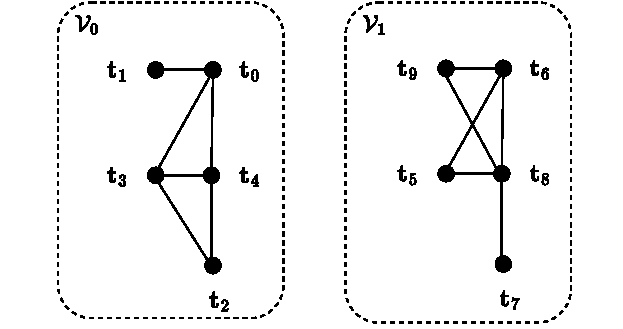
\includegraphics[width=0.5\textwidth]{fig/ch3/met4-eg}
		\caption{The undirected graph $U$ and the partitions $\mathcal{V}_0$ and $\mathcal{V}_1$. }
		\label{fig3:met4-eg-udg}
	\end{subfigure}
	\hfill
	\begin{subfigure}{0.9\textwidth}
		\centering
		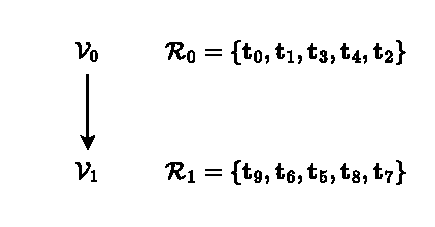
\includegraphics[width=0.35\textwidth]{fig/ch3/met4-eg-dfg}
		\caption{The graph $G'$ and the partial ranks.}
		\label{fig3:met4-eg-dfg}
	\end{subfigure}
	\caption{Methodology~\ref{th:problem4} on $\mathcal{M}_7$ and $<_{eg}$.  }
	\label{fig3:met4-eg}
\end{figure}

\textbf{Illustrative example:} Consider again the sets of measurements $\mathcal{M}_7$ and the relation $<_{eg}$. According to Step~1, the undirected graph $U$ consists of two partitions $\mathcal{V}_0$ and $\mathcal{V}_1$ (shown in Figure~\ref{fig3:met4-eg-udg}). The directed graph $G'$ and the resulting ordered set partitioning are shown in Figure~\ref{fig3:met4-eg-dfg}.   

\begin{mylem}{}{lemma4}
	Rankings produced by Methodology~\ref{th:problem4} are partial rankings (Def.~\ref{th:ranking}) and consists of minimum possible number of ranks.
	%Equation~\ref{eq:rank-sort} is a valid partial ranking according to Definition~\ref{th:ranking}. 
\end{mylem}
\textit{Proof:} Notice that $\forall \mathcal{R}_a, \mathcal{R}_b$, $a<b \implies \forall \mathbf{t}_k \in \mathcal{R}_a$ and $ \forall \mathbf{t}_l \in \mathcal{R}_b$, $\mathbf{t}_k <_{\mathbf{P}} \mathbf{t}_l$. Thus, the requirements according to Property~1 and Property~2 are satisfied. The condition according to Property~3 is naturally satisfied as all the variants in a particular partition $\mathcal{V}_i$ are connected by the incomparability relation $\sim$. Hence, the ranking computed according to Methodology~\ref{th:problem4} is a partial ranking.

Moreover, as all the variants in a particular rank are associated by $<_{\mathbf{P}}$ with all the variants in a subsequent rank, it is not possible to merge any two ranks; otherwise, the requirement according to Property~3 in Definition~\ref{th:ranking} would be violated. As all the variants in a particular rank are incomparable to one another, it is also not possible to split a rank into two (and somehow merge with other ranks); otherwise, the requirement according to Property~2 in Definition~\ref{th:ranking} would be violated. Hence, the partial ranking according to  Methodology~\ref{th:problem4} consists of minimum possible number of ranks. 
\begin{figure}[h!]
	\centering
	\begin{subfigure}{0.35\textwidth}
		\centering
		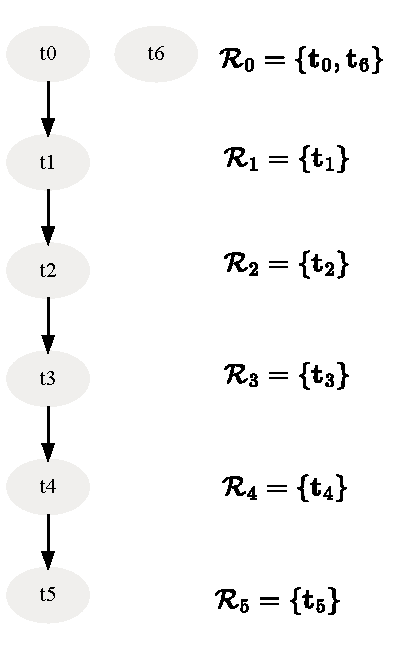
\includegraphics[width=0.8\textwidth]{fig/ch3/minrank-eg3-dfg}
		\caption{Methodology~\ref{th:problem2} on $\mathcal{M}_{9}$.}
		\label{fig3:minrank-eg3-dfg}
	\end{subfigure}
	
	\hfill
	
	\begin{subfigure}{0.85\textwidth}
		\centering
		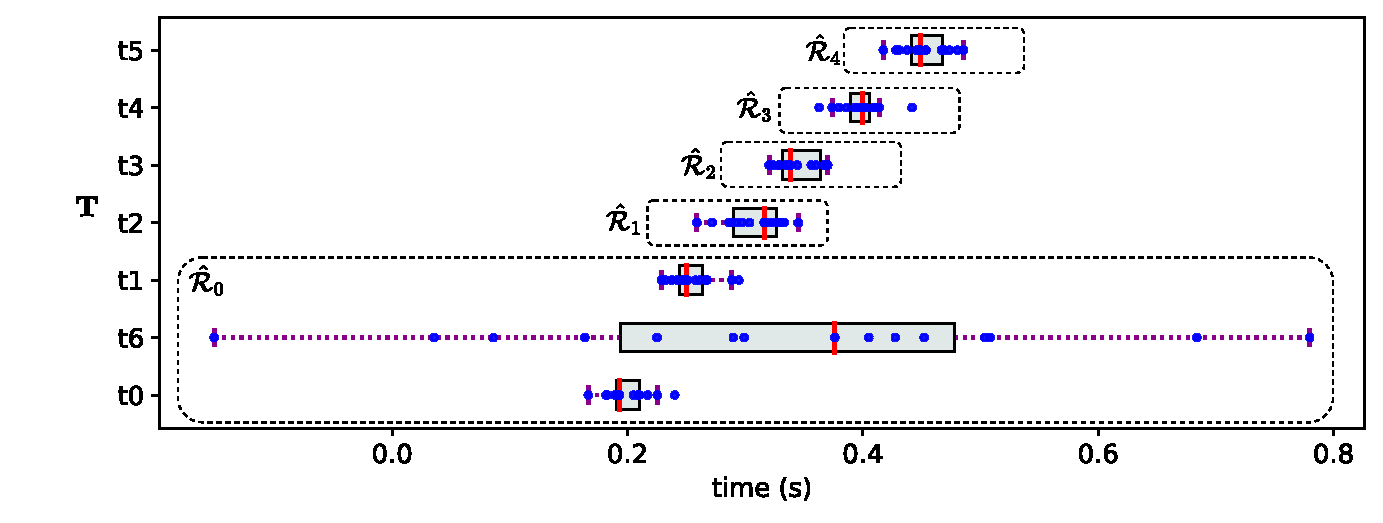
\includegraphics[width=0.8\textwidth]{fig/ch3/minrank-eg3-r}
		\caption{Methodology~\ref{th:problem3} on $\mathcal{M}_{9}$.}
		\label{fig3:minrank-eg3-r}
	\end{subfigure}
	
	\caption{Partial ranking of $\mathcal{M}_{9}$ with $<_{eg}$.  }
	\label{fig3:minrank-eg3}
\end{figure}

\subsection{Implications on some special cases:} 
When there are numerous variants with their measurement intervals distinctly separated from each other, except for a single variant whose interval overlaps with all the others, Methodology~\ref{th:problem4} merges all the variants into one rank. Such a ranking is sometimes undesired because it is not possible to discriminate between any of the distinctly separated variants as they are all tied by a single variant. 
For example, consider the sets of measurements $\mathcal{M}_{9}$ shown in Figure~\ref{fig3:minrank-eg3-r}. Each variant consists of 15 measurement values and the IQI of all the variants except for $\mathbf{t}_6$ are distinctly separated from one another. 
For $\mathcal{M}_{9}$, Methodology~\ref{th:problem2} produces a partial ranking with six ranks as shown in Figure~\ref{fig3:minrank-eg3-dfg}, and this is the maximum number of ranks that could be produced for $\mathcal{M}_{9}$ with $<_{eg}$; $\mathbf{t}_0, \mathbf{t}_6 \in \mathcal{R}_0$ and all the other variants in distinct ranks. Methodology~\ref{th:problem3} reduces the number of ranks by 1, and the resulting partial rankings are annotated in Figure~\ref{fig3:minrank-eg3-r}.
Methodology~\ref{th:problem4} however, produces a partial ranking where all the variants are placed in a single rank. %Therefore, for practical purposes, it is possible that Methodology~\ref{th:problem3} could be more useful than Methodology~\ref{th:problem4} despite not computing the minimum number of ranks. 


Let us examine one more example that showcases variants with overlapping yet monotonically increasing differences, such as the sets of measurements $\mathcal{M}_{10}$ depicted in Figure~\ref{fig3:minrank-eg5}. In this case, although assigning a distinct rank to each variant seems more intuitive\footnote{In this context, the way in which a ranking intuitively reflects the information present in the data.}, both Methodology~\ref{th:problem3} and Methodology~\ref{th:problem4} produces a partial ranking where all the variants are placed in the same rank (as shown in Figure~\ref{fig3:minrank-eg5-r}). Methodology~\ref{th:problem2} computes a partial ranking with 2 ranks (as shown in Figure~\ref{fig3:minrank-eg5-dfg}). Notice that Methodology~\ref{th:problem2} does not compute the maximum possible number of ranks, because for $\mathcal{M}_{10}$, the following partial ranking with 3 ranks exists: $\mathcal{R}_0 = \{\mathbf{t}_0, \mathbf{t}_1\}$,  $\mathcal{R}_1 = \{\mathbf{t}_2, \mathbf{t}_3\}$ and  $\mathcal{R}_2 = \{\mathbf{t}_4\}$.
 %Such a ranking could be avoided by choosing a different better-than relation instead of $<_{eg}$ (we elaborate on this further in subsequent section).

\begin{figure}[h!]
	\centering
	\begin{subfigure}{0.45\textwidth}
		\centering
		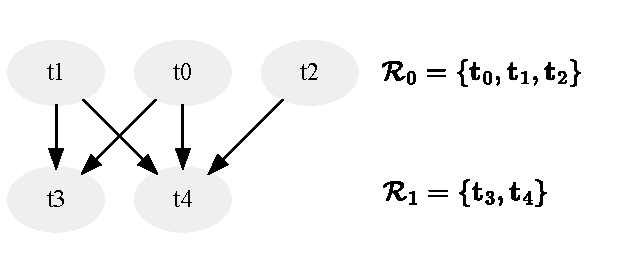
\includegraphics[width=\textwidth]{fig/ch3/minrank-eg5-dfg}
		\caption{Methodology~\ref{th:problem2} on $\mathcal{M}_{10}$.}
		\label{fig3:minrank-eg5-dfg}
	\end{subfigure}
	\hfill
	\begin{subfigure}{0.85\textwidth}
		\centering
		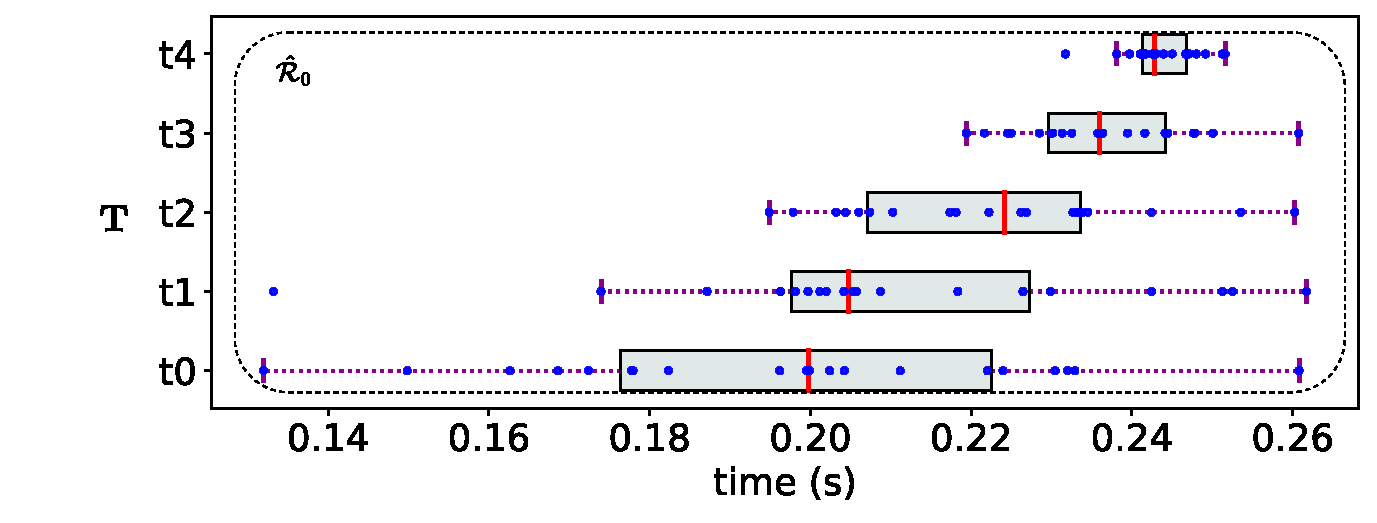
\includegraphics[width=0.8\textwidth]{fig/ch3/minrank-eg5-r}
		\caption{Methodology~\ref{th:problem3} on $\mathcal{M}_{10}$.}
		\label{fig3:minrank-eg5-r}
	\end{subfigure}
	\caption{Partial ranking of $\mathcal{M}_{10}$ with $<_{eg}$.  }
	\label{fig3:minrank-eg5}
\end{figure}





\section{Handling the effects of the Quantile Intervals }
\label{sec3:handlingq}
Thus far, we have utilized the relation $<_{eg}$ to compare two sets of measurements, which makes comparisons based on overlap in the Inter Quartile Intervals (IQIs), or in other words,  based on overlap in the Inter \textit{Quantile} Interval (IQnI) between the 25th and 75th quantiles among the variants. Sometimes, altering the quantiles can lead to a different ranking. 
%Modifying the quantiles used for computing the interval in the better-than relation can potentially alter the resulting partial ranking generated by a specific methodology.
For instance, consider the sets of measurements $\mathcal{M}_{11}$ shown in Figure~\ref{fig:rel-eg} where it could be intuitive for one to expect the following ranking:
\begin{equation}
\label{eq:rel-rank}
\mathcal{R}_0 =\{ \mathbf{t}_0, \mathbf{t}_2 \}, \quad \mathcal{R}_0 =\{ \mathbf{t}_1, \mathbf{t}_3 \}.
\end{equation}
%Consider the ranking computed by the Hasse-based methodology with $<_{eg}$  where
However, the IQnI between the 25th and the 75th quantile  of $\mathbf{t}_1$ \textit{slightly} overlaps with that of $\mathbf{t}_0$ and $\mathbf{t}_2$. As a consequence, when using the relation $<_{eg}$ to compare the variants,  $\mathbf{t}_0$, $\mathbf{t}_1$ and $\mathbf{t}_2$ are all pairwise incomparable and obtain the same rank.
In order to alleviate this problem, for a given ranking methodology, we compute multiple rankings corresponding to different quantiles, and average them. In what follows, we propose a systematic way of choosing a ranking corresponding to one among several quantile intervals based on the averaged or the mean ranks. 
\begin{figure}
	\centering
	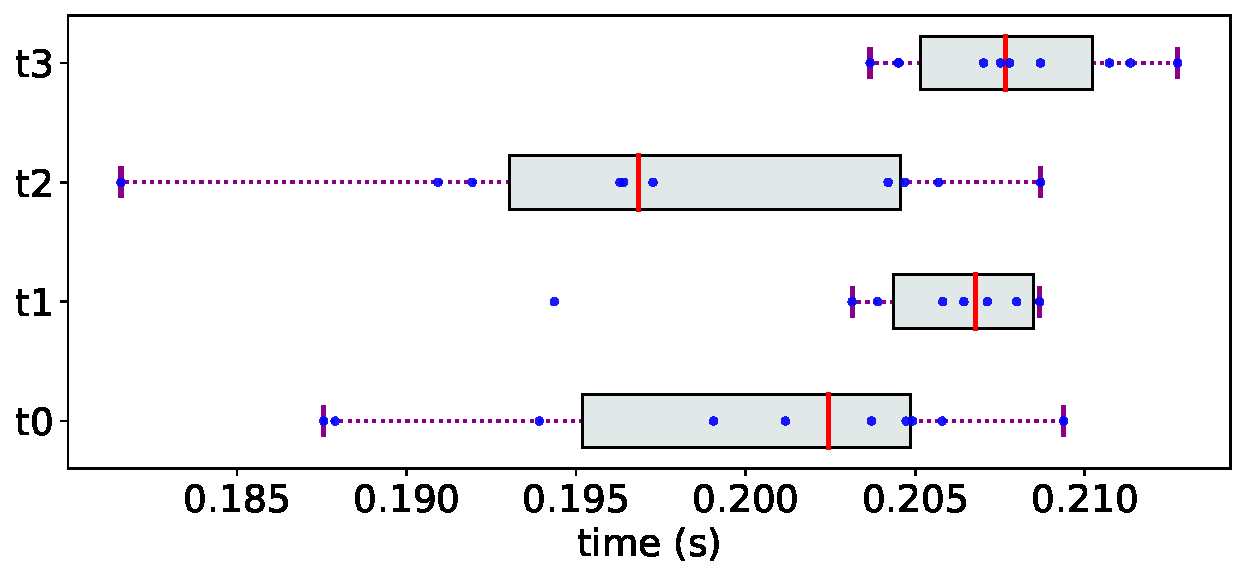
\includegraphics[width=0.6\linewidth]{fig/ch3/mean-rank-eg}
	\captionof{figure}{Sets of measurements $\mathcal{M}_{11}$.}
	\label{fig:rel-eg}
\end{figure}

%We aim to find the quantiles that results in a more \textit{reliable} ranking for a given ranking methodology and the sets of measurements.
To this end, let us first generalize $<_{eg}$ to accommodate arbitrary quantile limits. Let $l$ and $u$ denote  the lower and the upper quantile limit respectively. For each set of measurements values $\mathbf{t}_i \in \mathbb{R}^{M}$,  sort $\mathbf{t}_i$ in the ascending order and let $t_i^{l}, t_i^{u} \in \mathbb{R}$ be the linearly interpolated measurement values at the $l$ and $u$ quantiles respectively. Then, for each $\mathbf{t}_i$, $(t_i^{l}, t_i^{u})$ is the IQnI between the quantile limit $(l,u)$. We define the relation  $<_{(l,u)}$ as:

\begin{mydef}{$<_{(l,u)}$}{compare}
	For a given $(l, u)$, $\mathbf{t}_i <_{(l,u)} \mathbf{t}_j$ if and only if $t_i^{u} < t_j^{l}$.
\end{mydef}

\noindent  Thus, inferring from Definition~\ref{th:compare}, two sets of measurements are considered incomparable if and only if their IQnIs overlap with one another. If $l = 25$  and $u = 75$, then IQnI becomes the IQI indicated in our box plots; consequently, $<_{eg}$ is same as $<_{(25,75)}$.


Let $\mathcal{Q}$ be a set of quantile limits. For a given ranking methodology, let $r(\mathbf{t}_i, l, u)$ be the rank calculated for the variant $\mathbf{t}_i \in \mathcal{M}$ at a particular $(l, u) \in \mathcal{Q}$. As the choice of ($l, u$) influences the partial rank calculation, instead of computing a partial ranking at just one $(l,u)$, we compute the partial ranks at several quantile limits, i.e., $\forall (l,u) \in \mathcal{Q}$, and calculate the mean rank of each variant. Let the mean rank of $\mathbf{t}_i$ be denoted by $mr(\mathbf{t}_i)$. Then, the reliability score $rel(\mathbf{t}_i, l,u)$ of the rank assigned to the variant $\mathbf{t}_i$ at a particular quantile limit $(l,u)$ is defined as:
\begin{equation}
\label{eq:rel-eq}
rel(\mathbf{t}_i, l, u) = -|r(\mathbf{t}_i,l, u) - mr(\mathbf{t}_i)|
\end{equation}
where a higher reliability score can be considered as a better ranking for the given measurement data, a better-than relation and $\mathcal{Q}$. That is, for the variant $\mathbf{t}_i$, the lower the difference of the rank $r(\mathbf{t}_i, l,u)$ calculated at a particular $(l,u)$ from the mean of the ranks $mr(\mathbf{t}_i)$  calculated at several quantile limits, the higher the reliability score  $rel(\mathbf{t}_i, l, u)$, indicating that the rank assignment $r(\mathbf{t}_i, l,u)$ is more reliable. The average reliability (avg\_rel) of a partial ranking at a quantile limit $(l,u)$ is the mean of the reliability scores at that $(l,u)$ from all the variants; that is,
\begin{equation}
\text{avg\_rel}(l,u) = \frac{\sum\limits_{\mathbf{t}_i} rel(\mathbf{t}_i, l, u)}{|\mathcal{M}|} 
\end{equation}
where $|\mathcal{M}|$ is the total number of objects.


Thus, given $\mathcal{Q}$, we propose to compute partial rankings and average reliability scores $\forall (l,u) \in \mathcal{Q}$, and select a ranking with the highest average reliability score. 
%It is important to choose $\mathcal{Q}$ carefully to ensure they serve the purpose of ranking effectively; for instance, choosing limits such as $(49,51)$ or $(0,5)$ is unreasonable when the purpose is to account for ties, because then, the better-than relation approximates a ranking based on median or minimum and disregards ties. 

\begin{table}[h!]
	\centering
	\begin{adjustbox}{width=0.65\columnwidth,center}
		\begin{tabular}{@{}ll ccccccccc@{}}
			\toprule
			&&$\mathbf{t}_0$ &&$\mathbf{t}_1$ &&$\mathbf{t}_2$ &&$\mathbf{t}_3$ &&avg\_rel$(l,u)$ \\
			\midrule
			$r(\mathbf{t}_i,25,75)$&& 0&&0&&0&&1&&-\\
			$r(\mathbf{t}_i,30,70)$&& 0&&1&&0&&1&&-\\
			$r(\mathbf{t}_i,35,65)$&& 0&&1&&0&&1&&-\\
			$r(\mathbf{t}_i,40,60)$&& 1&&2&&0&&2&&-\\
			\midrule
			$mr(\mathbf{t}_i)$ &&0.25&&1.00&&0.00&&1.25&&-\\
			\midrule
			$rel(\mathbf{t}_i,25,75)$&& -0.25&&-1.0&&0.0&&-0.25&&\textbf{-0.38}\\
			$rel(\mathbf{t}_i,30,70)$&& -0.25&&-0.00&&0.0&&-0.25&&\textbf{-0.13}\\
			$rel(\mathbf{t}_i,35,65)$&& -0.25&&-0.00&&0.0&&-0.25&&\textbf{-0.13}\\
			$rel(\mathbf{t}_i,40,60)$&& -0.75&&-1.00&&0.0&&-1.25&&\textbf{-0.75}\\
			\bottomrule
		\end{tabular}
	\end{adjustbox}
	\caption{Reliability Scores of the ranks computed by Methodology~\ref{th:problem2} on $\mathcal{M}_{11}$ with $<_{(l,u)}$ at different quantile limits.}
	\label{tab:rel}
\end{table}

\paragraph{Illustrative Example:}
%to calculate a score for the ranks such that any ranking that consists of $\mathcal{R}_0 = \{\mathbf{t}_0, \mathbf{t}_1, \mathbf{t}_2\}$ 
%to quantify the reliability of the calculated ranks in terms of reliability of $<_p$. 

Let us compute partial rankings for $\mathcal{M}_{11}$ using Methodology~\ref{th:problem2} at all
\begin{equation}
\label{eq:qlist}
(l, u) \in  \{ (25,75), (30,70), (35,65), (40,60) \}.
\end{equation}
The mean ranks of the variants, the reliability scores of the rank assignments and the average reliability scores are shown in Table~\ref{tab:rel}.   The partial rankings at the limits $(30,70)$ and $(35, 65)$, which classifies the variants into ranks as expected according to Eq.~\ref{eq:rel-rank}, obtains a higher average reliability score than the partial rankings at other limits. 


\section{Experiments: Mining for the causes of performance differences from the measurement data}  
\label{sec3:exp}

Partial ranking of a set of objects can be seen as clustering the objects into performance classes; i.e., a clustering in which there is a notion of one cluster being better than another.
% Performance classes arise in a variety of applications; for instance, in~\cite{marker2014understanding}, Marker et al. observes that the performance of  algorithmic variants of Dense Linear Algebra problems are often stair-stepped, i.e., they occur in performance classes, where each class consists of a set of variants with very similar performance. When analyzing business processes, one of the important functionalities provided by software tools is the ability to filter process variants based on their performance~\cite{van_der_aalst2016process}.
 In this section, we demonstrate that identifying performance classes using our partial ranking methodologies automate the discovery of the causes of performance differences between the variants. For our experiments, we revisit the execution time measurements of the algorithmic variants of the Generalized Least Square (GLS) problem introduced in Section~\ref{sec3:int}, and identify the library calls that impact performance the most (Section~\ref{sec3:gls}). Then,  we apply our partial ranking methodology on a real-life dataset from a Business Process application to identify the underlying causes of inefficiencies (Section~\ref{sec3:bpi}).

%As a side track from algorithm selection and to prove the general applicability of our approach,  we also consider a Business process example from a real life data gathered from a SAP system, and aim to identify root causes of inefficiencies. 

% For example, consider the Generalized Least Squares problem (GLS); mathematically, this is expressed by the assignment:
% \begin{equation}
% \label{eq3:matchain}
% b := (X^{T}M^{-1}X)^{-1}X^{T}M^{-1}y
% \end{equation}
% where $X \in \mathbb{R}^{m\times n}$, $M \in \mathbb{R}^{m\times m}$ and $y \in \mathbb{R}^{m}$. An algorithm to compute assignment~\ref{eq:matchain} can be identified as a sequence of invocations to linear algebra building block kernels such as those provided by BLAS and LAPACK~\cite{dongarra1985proposal,demmel1991lapack
% }. In general, for a given expression, many different  kernel sequences exists (sometimes over hundreds), all mathematically equivalent but exhibiting different performance signatures~\cite{Psarras2022:618}. Each algorithmic variant consists of some sequence of kernel invocations. Expression compilers such as Linnea~\cite{barthels2021linnea} can automatically generate those algorithmic variants. We consider a subset of algorithms generated by Linnea for~(\ref{eq3:matchain}). For operand sizes $m=1000$ and  $n=100$, the execution time of each algorithm was measured 10 times\footnote{The repetitions of each algorithm were not consecutive, but shuffled among other algorithms.} on a Linux-based system using 12 cores of an Intel Xeon processor. The measurements are shown as box plots in Fig~\ref{fig:time}\footnote{Even though the experiments were run on a compute environment with exclusive access, one could still observe instability in the measurements, likely due to contention with other processes launched by the Operating System, and because of the effects of turbo boost.}. 

\subsection{Algorithmic Variants of GLS}
\label{sec3:gls}

The execution time measurements of ten algorithmic variants of GLS for given matrix dimensions are shown again in Figure~\ref{fig3:gls-eg}. Each algorithmic variant can be identified as a sequence of library or kernel calls provided by optimized libraries such as BLAS and LAPACK. The sequences of kernel calls for the ten algorithmic variants as generated by the Linnea compiler~\cite{barthels2021linnea} are shown in Table~\ref{tab3:gls-seq}.
%The computation of the GLS expression can be accomplished using one of the many algorithmic variants, each identified by a sequence of invocations to linear algebra building block kernels provided by the BLAS and LAPACK libraries. Let us revisit the ten algorithmic variants for GLS for operand sizes $m=1000, n=100$ discussed in Chapter~1 (Table~\ref{tab:ch1-vars}). The kernel sequences of those variants are shown in Table~\ref{tab3:gls-seq}, and the corresponding execution time measurements ($\mathcal{M}_{gls}$) are shown again in Figure~\ref{fig3:gls-eg}. 
Let us first attempt to elucidate the causes of performance differences among the variants in terms of the kernel calls, solely by looking at the data $\mathcal{M}_{gls}$, without relying on any specific ranking methodology. At first glance, one could intuitively categorize the variants into two distinct groups: Fast variants  and Slow variants, as represented  below:
\begin{equation}
\label{eq3:gls-gt}
\begin{aligned}
\text{Fast} &= \{\mathbf{alg}_0, \mathbf{alg}_1, \mathbf{alg}_3, \mathbf{alg}_4, \mathbf{alg}_5\} \\
\text{Slow} &= \{\mathbf{alg}_2, \mathbf{alg}_6, \mathbf{alg}_7, \mathbf{alg}_8, \mathbf{alg}_9\}
\end{aligned}
\end{equation}

%We aim to explain the causes of performance differences among the variants in terms of the kernel calls using $\mathcal{M}_{gls}$. 
%
%We use the Linnea compiler to automatically generate  the algorithmic variants for GLS. We show the 
%
% We would like to identify the causes of performance differences among the variants in terms of those kernel calls. 
%
%Recall than an algorithm to compute the GLS expression (Expression~\ref{eq:gls}) can be identified as a sequence of invocation to linear algebra
%building block kernels provided by the BLAS and LAPACK libraries. In general, for a given expression, many different mathematically equivalent kernel sequences exists, and each such sequence is an algorithmic variant. We aim to explain the root causes of performance differences among the variants in terms of the kernel calls. To this end, let us consider the ten algorithmic variants for Expression~\ref{eq:gls}, whose details were listed in Table~\ref{tab:ch1-vars}. The set of distribution  of execution time measurements of those variants are shown again in Figure~\ref{fig3:gls-eg}, and let us denote it as $\mathcal{M}_{gls}$. Using the data $\mathcal{M}_{gls}$, we would like to identify the causes of performance differences among the variants in terms of the kernel calls. 


\begin{table}[!t]
		\begin{minipage}{1\textwidth}
		\centering
		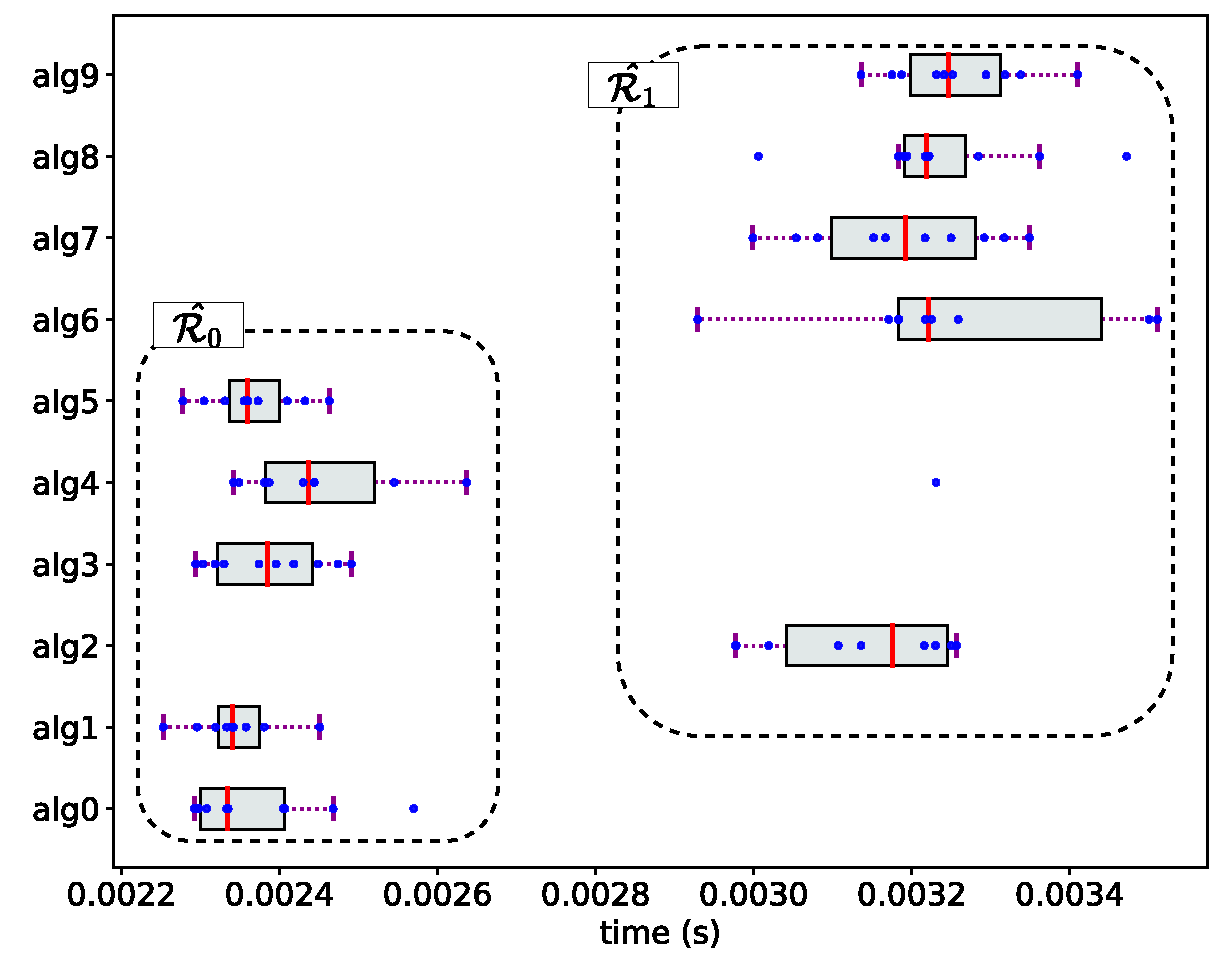
\includegraphics[width=0.6\linewidth]{fig/ch3/gls-eg}
		\captionof{figure}{The  time measurements of the algorithmic variants of the GLS problem:  $(X^{T}M^{-1}X)^{-1}X^{T}M^{-1}\mathbf{y}$ where  $X \in \mathbb{R}^{1000 \times 100}$, $M \in \mathbb{R}^{1000 \times 1000}$ and $\mathbf{y} \in \mathbb{R}^{1000}$ ($\mathcal{M}_{gls}$). The partial rankings using Methodology~\ref{th:problem3} according to $<_{eg}$ are annotated.}
		\label{fig3:gls-eg}
	\end{minipage}
\hfill
\bigskip

	\begin{minipage}{1\textwidth}
		\centering
		\begin{adjustbox}{width=0.65\columnwidth,center}
			\begin{tabular}{@{}l cc@{}}
				\toprule
				\textbf{Variant} &&\textbf{Kernel sequence}\\
				\midrule
				$\mathbf{alg}_0$&& potrf, trsm, trsv, syrk, gemv, potrf, trsv, trsv \\
				$\mathbf{alg}_1$&& potrf, trsv, trsm, syrk, potrf, gemv, trsv, trsv\\
				$\mathbf{alg}_{2}$&& potrf, trsm, trsv, syrk, gemv, qr, gemv, trsv\\
				$\mathbf{alg}_{3}$&& potrf, trsv, trsm, gemm, potrf, gemv, trsv, trsv \\
				$\mathbf{alg}_{4}$&& potrf, trsm, trsv, gemm, gemv, potrf, trsv, trsv \\
				$\mathbf{alg}_{5}$&&  potrf, trsm, trsv, gemm, potrf, gemv, trsv, trsv \\
				$\mathbf{alg}_{6}$&& transpose, potrf, trsm, trsv, syrk, potrf, trsv, trsm, gemv, trsv\\
				$\mathbf{alg}_{7}$&& transpose, potrf, trsm, syrk, potrf, trsv, trsv, trsm, gemv, trsv \\
				$\mathbf{alg}_{8}$&& transpose, potrf, trsm, syrk, potrf, trsm, trsm, trsv, trsv, gemv \\
				$\mathbf{alg}_{9}$&&  transpose, potrf, trsm, syrk, potrf, trsv, trsv, trsm, trsm, gemv \\
				\bottomrule
			\end{tabular}
		\end{adjustbox}
		\captionof{table}{Kernel sequences of the ten algorithmic variants considered in Figure~\ref{fig3:gls-eg}.}
		\label{tab3:gls-seq}
	\end{minipage}
	%\hfill
	
\end{table}


% \begin{table}[!h]
% 	\begin{minipage}{.5\textwidth}
% 		\centering
% 		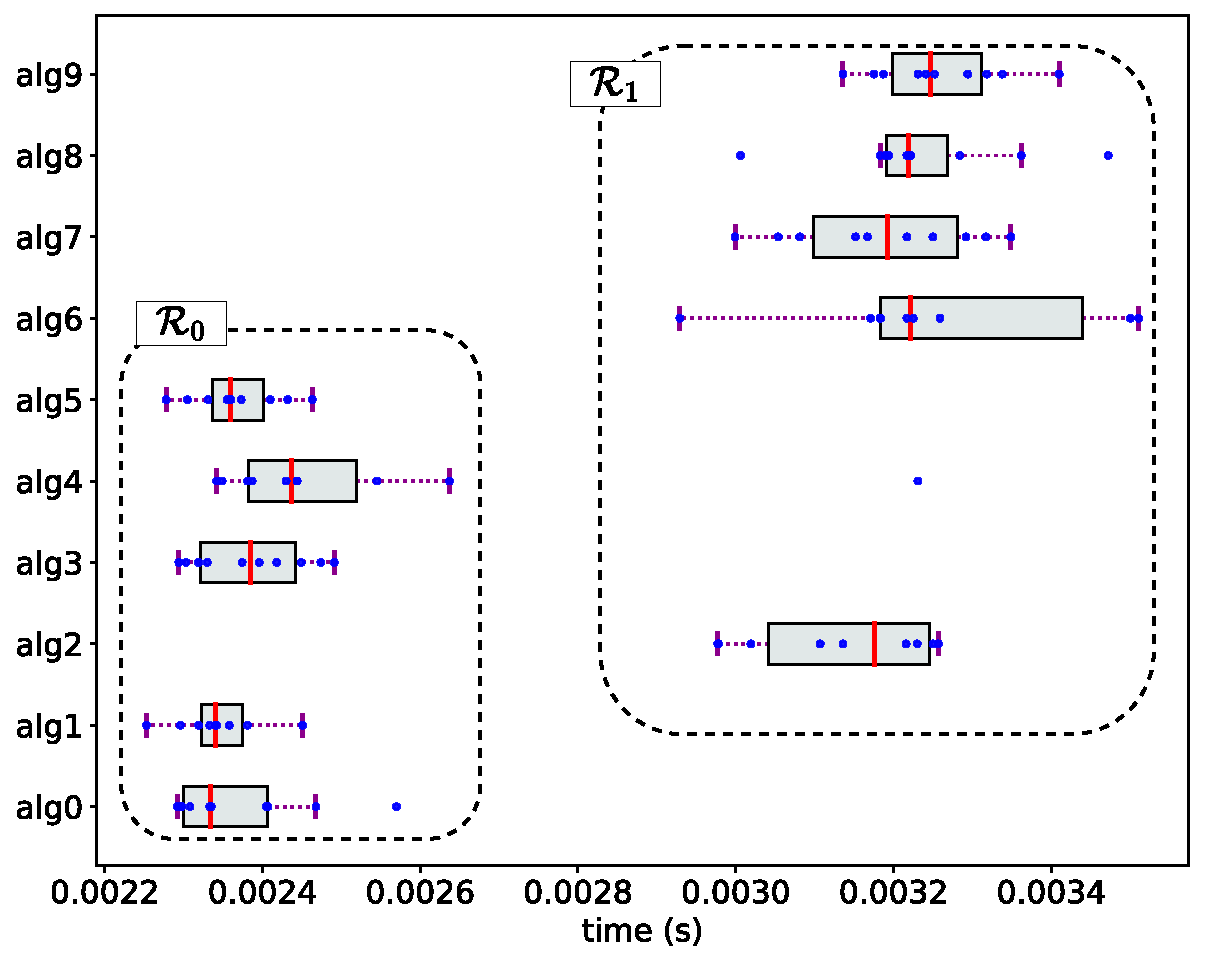
\includegraphics[width=1\linewidth]{fig/ch3/gls-1000-100-box2}
% 		\captionof{figure}{Time measurements for the algorithmic variants of GLS ($\mathcal{M}_{gls}$).\acc{TODO: change $\mathcal{R}$ to $\hat{\mathcal{R}}$}}
% 		\label{fig3:gls-eg}
% 		\centering
% 		\bigskip
% 		\begin{adjustbox}{width=0.65\columnwidth,center}
% 			\begin{tabular}{@{}l cccccc@{}}
% 				\toprule
% 				\textbf{Variant} && MFLOPs&&$\mathbf{M}_2$&& $\mathbf{M}_3$\\
% 				\midrule
% 				$\mathbf{alg}_0$&&$445$&&0&&0\\
% 				$\mathbf{alg}_1$&&$445$&&0&&0\\
% 				$\mathbf{alg}_{2}$&&$447$&&2&&1\\
% 				$\mathbf{alg}_{3}$&&$455$&&0&&0\\
% 				$\mathbf{alg}_{4}$&&$455$&&1&&0\\
% 				$\mathbf{alg}_{5}$&&$455$&&0&&0\\
% 				$\mathbf{alg}_{6}$&&$456$&&2&&1\\
% 				$\mathbf{alg}_{7}$&&$456$&&2&&1\\
% 				$\mathbf{alg}_{8}$&&$466$&&2&&1\\
% 				$\mathbf{alg}_{9}$&&$466$&&2&&1\\
% 				\bottomrule
% 			\end{tabular}
% 		\end{adjustbox}
% 	 		\captionof{table}{Partial Rankings of $\mathcal{M}_{gls}$ according to $<_{eg}$. 
% 	 			%The FLOP count for each algorithm is indicated in Mega FLOPs (MFLOPs). 
%  			 }
% 		\label{tab:ranks}
% 		
% 	\end{minipage}%
% 	\begin{minipage}{.5\textwidth}
% 		\centering
% 		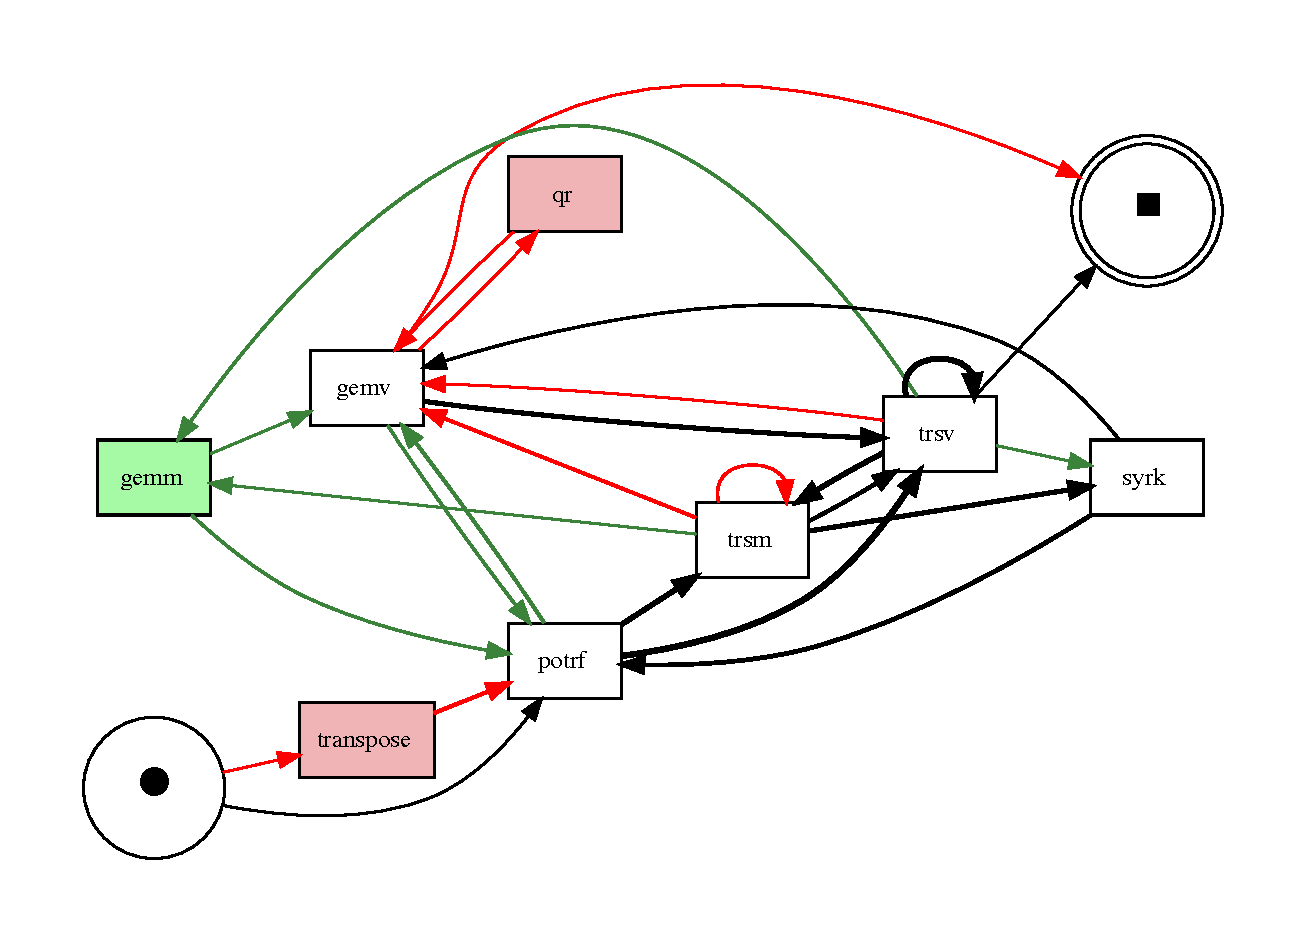
\includegraphics[width=.70\linewidth]{fig/ch3/gls-1000-100-dfg}
% 		\captionof{figure}{DFG: Green = $\hat{\mathcal{R}}_0$,\\ Red = $\{\mathbf{alg}_{2}\}$.}
% 		\label{fig:dfg-f}
% 	\end{minipage}
% \end{table}
By carefully observing the similarities and differences in the kernel sequences among the variants in the Fast and Slow groups based on the data $\mathcal{M}_{gls}$, one could discern the following associations:
\begin{enumerate}
	\itemsep0em 
	\item[\textbf{r1)}] Only the fast variants make use of the kernel \textit{gemm}.
	\item[\textbf{r2)}] Only the slow variants make use of the kernel \textit{transpose}.
	\item[\textbf{r3)}] Only the slow variants make use of the kernel \textit{qr}.
\end{enumerate}

This example is intentionally simplistic, but in reality, it is common to encounter hundreds of algorithmic variants with much longer kernel sequences for each variant. The manual process of making such discernments, even for this straightforward example, can be time-consuming and laborious. Therefore, given $\mathcal{M}_{gls}$ and the information regarding the kernel sequences in Table~\ref{tab3:gls-seq}, our objective is to automate the identification of the observations \textbf{r1}, \textbf{r2} and \textbf{r3} that we just manually discerned, and potentially uncover additional kernel sequence patterns that may have gone unnoticed during the manual analysis.

\begin{figure}[t!]
	\centering
	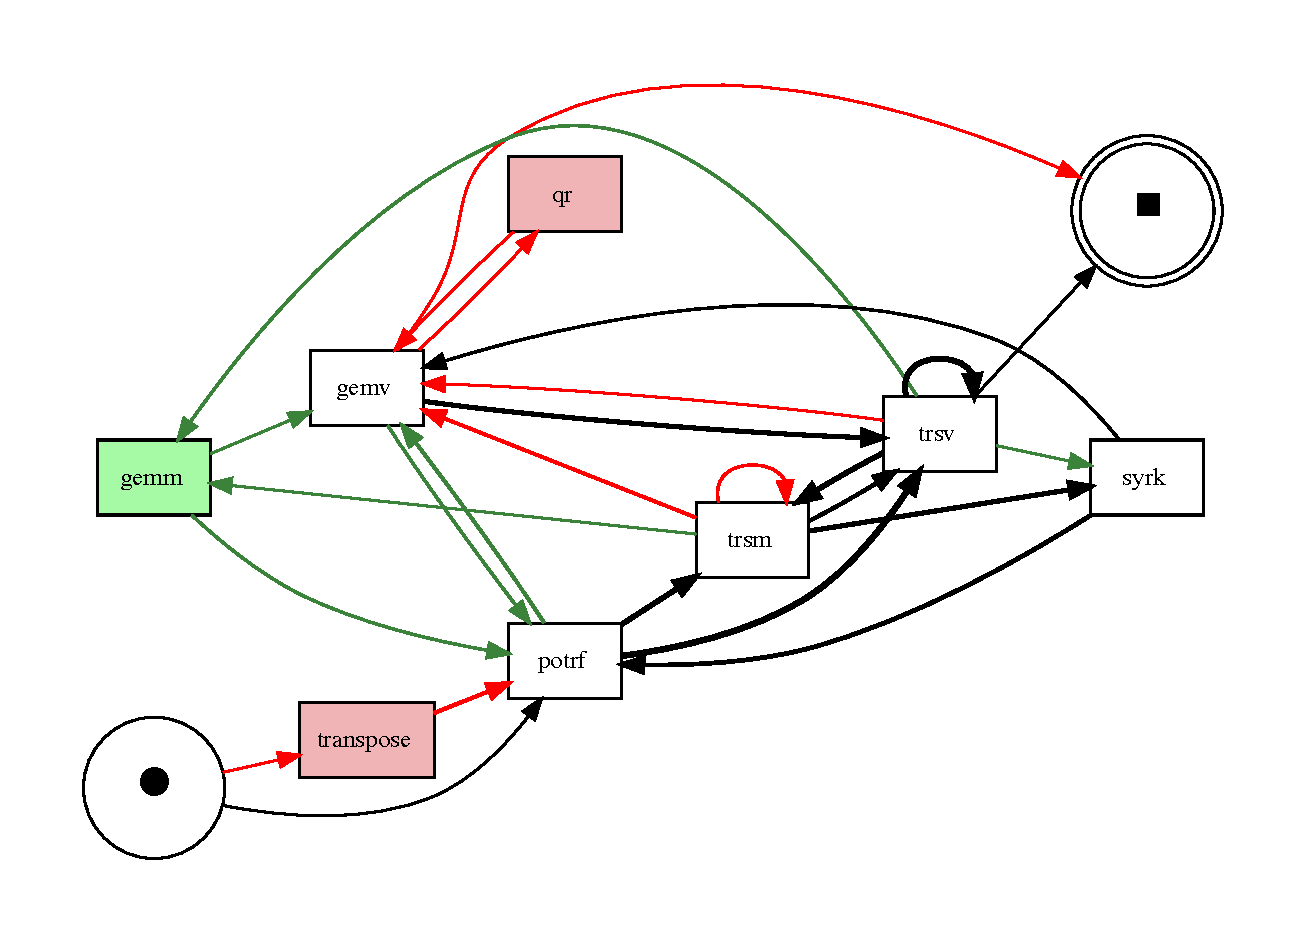
\includegraphics[width=.70\linewidth]{fig/ch3/gls-1000-100-dfg}
	\caption{Directly Follows Graph: $\mathcal{G}reen$ = $\hat{\mathcal{R}}_0$, $\mathcal{R}ed$ = $\mathcal{\hat{R}}_1$.}
	\label{fig:dfg-f}
\end{figure}

In Figure~\ref{fig3:gls-eg}, we notice two well-separated groups (whether or not the data occurs in well-separated clusters can be automatically determined using a pre-trained binary classifier~\cite{kumari2017machine}), and we want to limit the number of ranks to the count of the well-separated groups, without unnecessarily creating additional ranks. Therefore, we apply Methodology~\ref{th:problem3} on  $\mathcal{M}_{gls}$ using the better-than relation $<_{eg}$, creating a partial ranking of the variants.
The resulting ranks ---$\mathcal{\hat{R}}_0$ and $\mathcal{\hat{R}}_1$--- are annotated in Figure~\ref{fig3:gls-eg}. $\mathcal{\hat{R}}_0$ and $\mathcal{\hat{R}}_1$ are incidentally same as the manually identified Fast and Slow sets (shown in Equation~\ref{eq3:gls-gt}) respectively. 

\begin{figure}[h!]
	\centering
	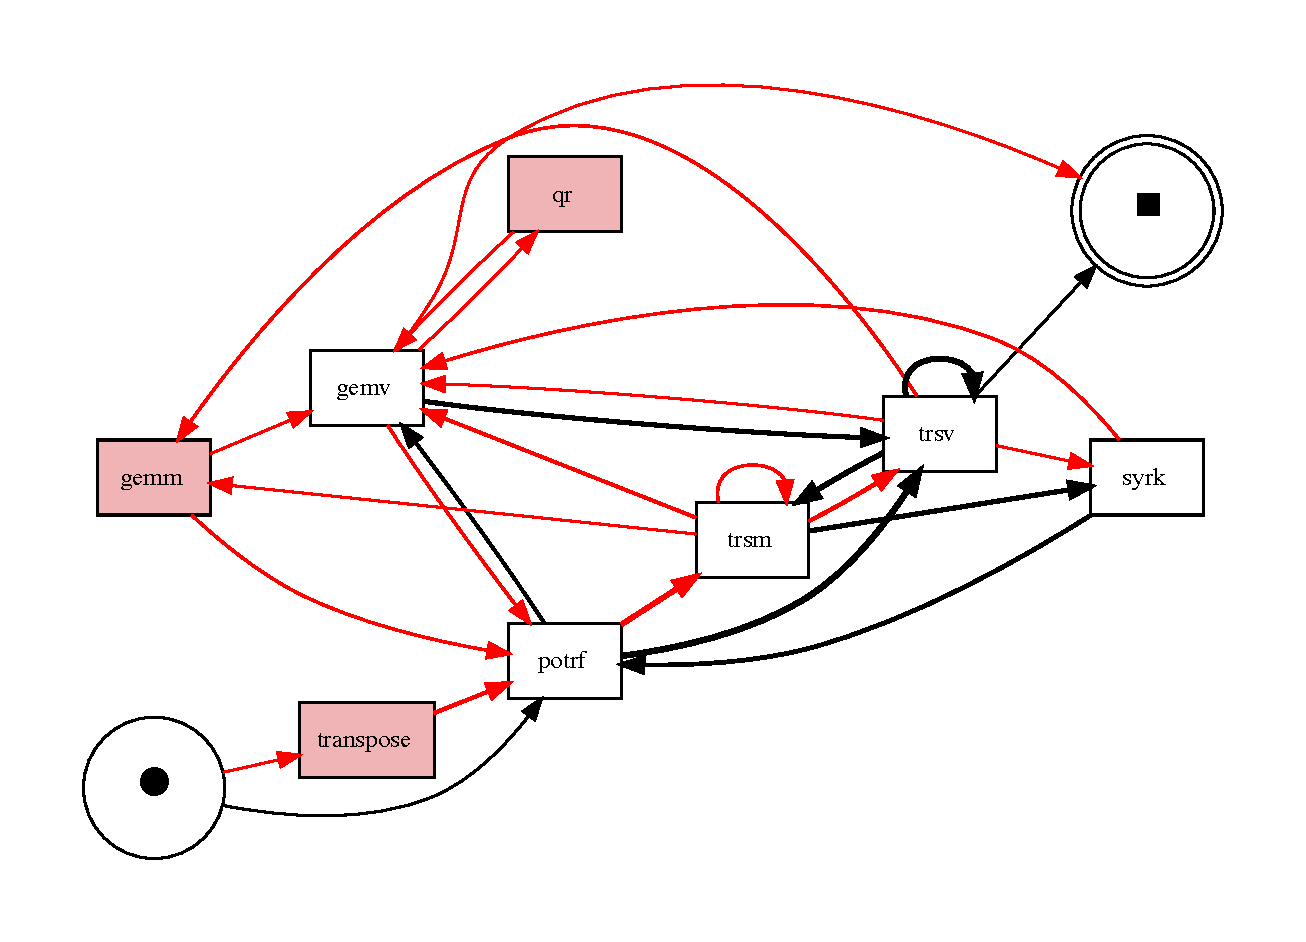
\includegraphics[width=.7\linewidth]{fig/ch3/gls-median}
	\caption{DFG (Top-1 median ranking):  $\mathcal{G}reen = \{ \mathbf{alg}_0\}$, $\mathcal{R}ed$ contains the remaining variants.}
	\label{fig3:dfg-m1}
\end{figure}



In order to identify the similarities and differences among the variants in $\mathcal{\hat{R}}_0$ and $\mathcal{\hat{R}}_1$ in terms of kernel calls, we construct a Directly-Follows-Graph (DFG), where each node indicates a kernel, and a directed edge from one kernel to another, say from \textit{kernelA} to \textit{kernelB}, indicates that there exists a kernel sequence in which \textit{kernelA} directly precedes \textit{kernelB}. Given a split of the variants into two sets $\mathcal{G}reen$ and $\mathcal{R}ed$, we color the nodes and edges in the DFG such that green nodes and edges indicate the kernels and the directly-follows relations that occur \textit{exclusively} in the variants from $\mathcal{G}reen$. Similarly, red nodes and edges indicate the kernels and the directly-follows relations that occur exclusively in the variants from $\mathcal{R}ed$. All the other kernels and relations occur in the variants from both $\mathcal{G}reen$ and $\mathcal{R}ed$. The DFG with $\mathcal{G}reen = \hat{\mathcal{R}}_0$ and  $\mathcal{R}ed$ = $\mathcal{\hat{R}}_1$ is shown in Figure~\ref{fig:dfg-f}. The kernel \textit{gemm} that occurs only in the variants from $\hat{\mathcal{R}}_0$ is colored green, and the kernels \textit{transpose} and \textit{qr} that occurs only in the variants from $\hat{\mathcal{R}}_1$ is colored red. Hence, we automatically identify the observations \textbf{r1}, \textbf{r2} and \textbf{r3}. We also discover additional patterns, such as the observation that whenever the kernels \textit{trsm} or \textit{trsv} directly precede \textit{gemv}, the corresponding variant is not one of the fast ones.

\begin{figure}[h!]
	\centering
	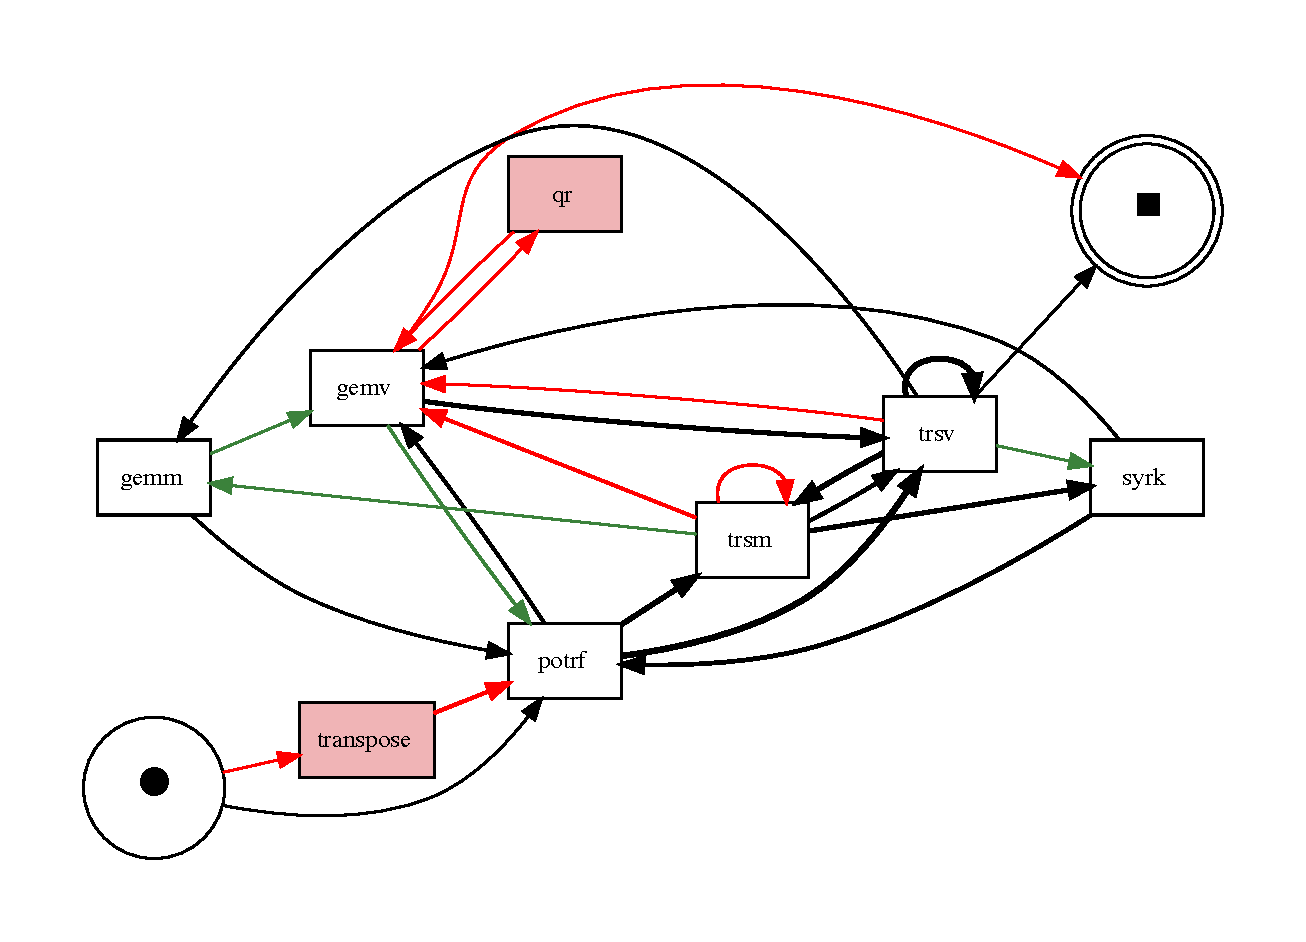
\includegraphics[width=.7\linewidth]{fig/ch3/gls-top4}
	\caption{DFG (Top-4 median ranking):  \\ $\mathcal{G}reen = \{ \mathbf{alg}_0, \mathbf{alg}_1, \mathbf{alg}_5, \mathbf{alg}_3\}$, $\mathcal{R}ed$ contains the remaining variants.}
	\label{fig3:dfg-m4}
\end{figure}

In order to highlight the significance of using a ranking methodology that accounts for ties, we illustrate the limitations that are inherent when mining for the causes of performance difference based on rankings that determined by simply relying only on the median execution time of the variants. To this end, we consider the following:
\begin{itemize}
	\item \textbf{Top-1 median}: The variant having the lowest median execution time is placed in the set $\mathcal{G}reen$. The remaining variants are placed in the set $\mathcal{R}ed$. The resulting DFG is shown in the Figure~\ref{fig3:dfg-m1}. As this kind of ranking completely ignores ties, the coloring of the DFG is not reasonable; the kernel \textit{gemm} is colored red because the only variant in the set $\mathcal{G}reen$, which is $\mathbf{alg}_0$, does not use this kernel.  However, there exists other variants --- $\mathbf{alg}_3$, $\mathbf{alg}_4$ and $\mathbf{alg}_5$ --- that use \textit{gemm} and the spread of their execution times significantly overlaps with that of $\mathbf{alg}_0$. Hence, according to the available data, it is not reasonable to highlight \textit{gemm} as a cause for a variant to be slow. 
	\item \textbf{Top-k median}: Top-k ranking is a common approach to distinguish between good and bad variants. Here, the variants with the top $k$ lowest median execution times are placed in the set $\mathcal{G}reen$ and the remaining variants are placed in the set $\mathcal{R}ed$. It is important to note that in this context, the identification of reasonable causes depends on the choice of k. For $k=5$, the variants are split into the two sets according to ones intuition (i.e., according to Equation~\ref{eq3:gls-gt}). However, for $k=4$, we get the DFG shown in Figure~\ref{fig3:dfg-m4} in which the association \textbf{r1} is not identified. 
\end{itemize}




\subsection{Business Process Example}
\label{sec3:bpi}
Just as an algorithm can be viewed as a sequence of kernel calls, a business process can be viewed as a sequence of tasks or activities that need to be performed to achieve a specific business objective. For example, let us consider the Purchase-to-Pay (P2P)  business process, which involves the activities encountered while acquiring goods or services from external suppliers. This is a common business process carried out in many companies and organizations, which involves a series of interdependent activities that are performed by various entities within an organization. For every purchase request, the sequence in which the activities are executed is captured  by sophisticated Enterprise Resource Management systems like SAP. A particular sequence of activities is referred to as a process variant, and in large organizations, there are typically hundreds of process variants for a business process like P2P (in the following, we show an example). Making organizational changes to improve such a process often entails the use of several enterprise tools which facilitate in identifying the activities that contribute to process variants exhibiting specific performance issues, such as higher throughput time~\cite{van_der_aalst2016process}.

\begin{figure}[h!]
	\centering
	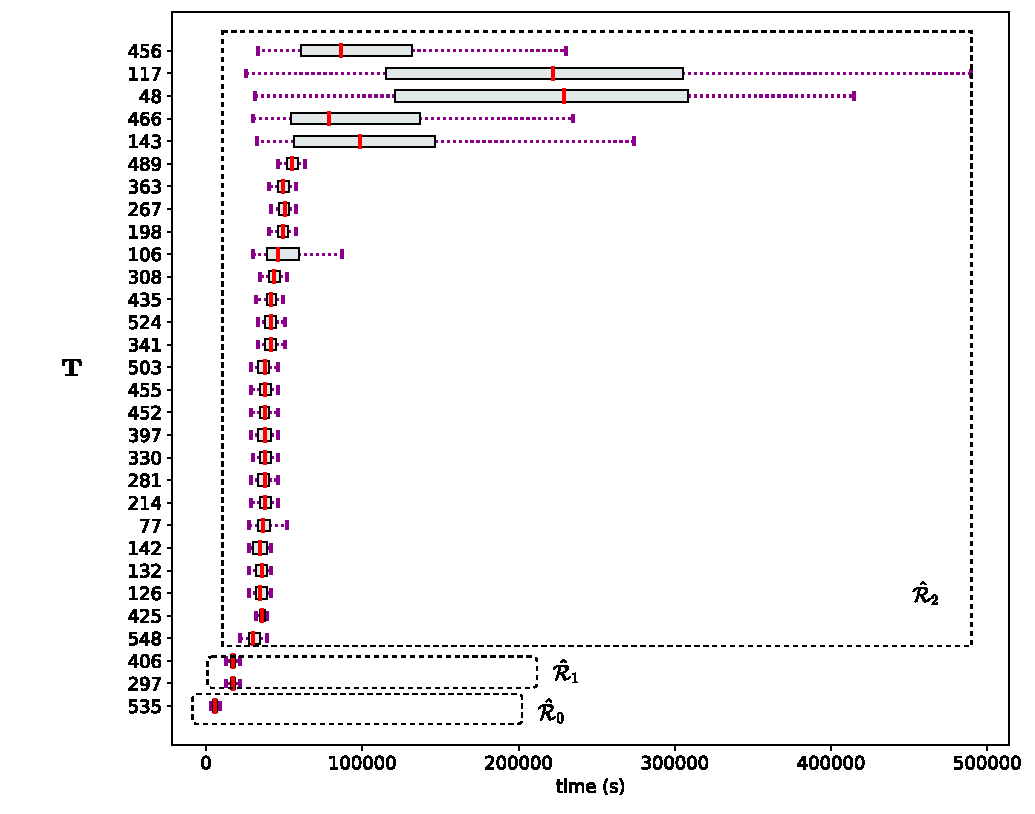
\includegraphics[width=0.8\textwidth]{fig/ch3/bpi-eg}
	\caption{Sets of throughput times of the process variants ($\mathcal{M}_{bpi}$) and the partial ranking annotated based on Methodology~\ref{th:problem3} according to $<_{eg}$.}
	\label{fig3:bpi-eg}
\end{figure}

\begin{figure}[h!]
	\centering
	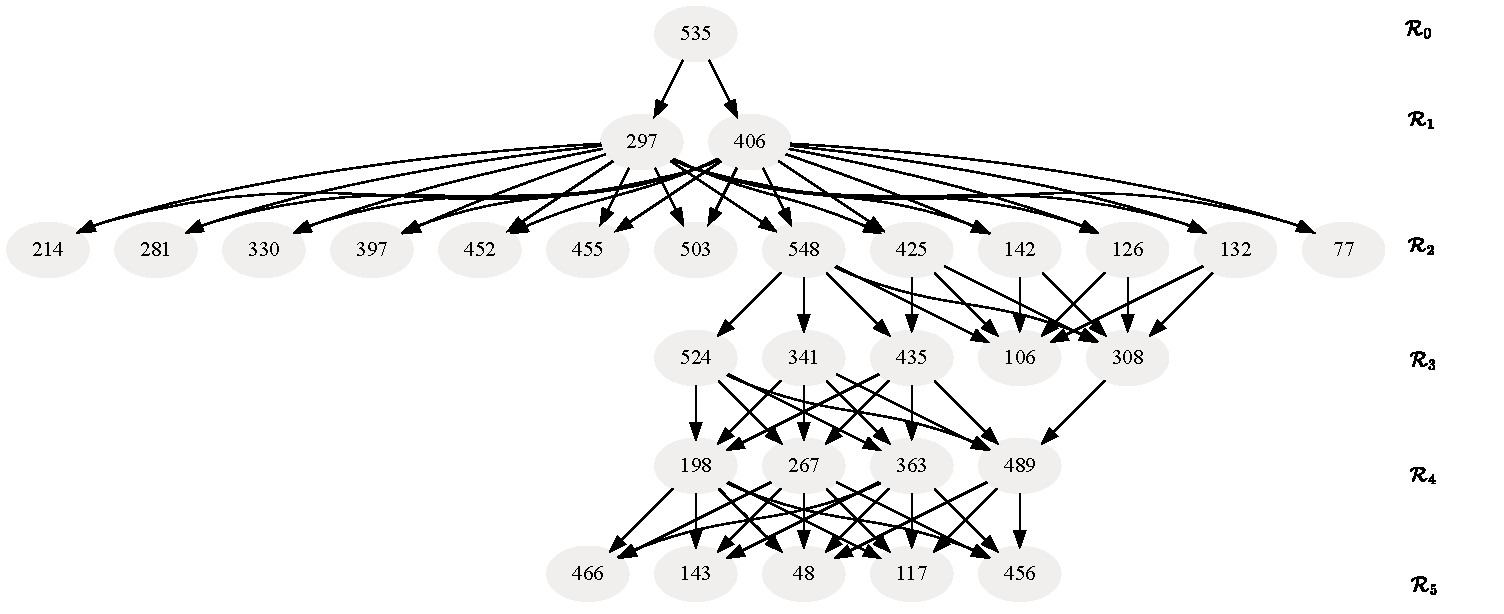
\includegraphics[width=\textwidth]{fig/ch3/bpi-eg-dfg}
	\caption{Methodology~\ref{th:problem2} on $\mathcal{M}_{bpi}$ according to $<_{eg}$. The graph $H$ is shown.}
	\label{fig3:bpi-eg-dfg}
\end{figure}

For the purpose of illustration, we consider a P2P dataset from certain organization provided by a German data processing company - Celonis\footnote{Celonis technology solutions are utilized by prominent organizations such as Exxon Mobil, BMW, General Electric, and many others~\cite{businesswire2019celonis}.}, during a hackathon event organized in collaboration with RWTH Aachen University in April 2022. 
%https://www.businesswire.com/news/home/20190114005089/en/Celonis-Gains-New-Customers-Across-Industries-and-Geographies-with-Its-Recently-Released-Intelligent-Business-Cloud
In the considered dataset,  the sets of throughput times of  the 30 most frequent process variants are shown in Figure~\ref{fig3:bpi-eg} ($\mathcal{M}_{bpi}$). The partial ranking according to Methodology~\ref{th:problem3} with $<_{eg}$ is annotated in Figure~\ref{fig3:bpi-eg}. However, as the spreads of the throughput times are largely overlapping with monotonically increasing differences, Methodology~\ref{th:problem3} and \ref{th:problem4} merges variants with significantly different performance into the same rank $\mathcal{\hat{R}}_2$. Moreover, the throughput times of the variants do not occur in well-separated groups. Therefore, instead of Methodology~\ref{th:problem3}, we employ Methodology~\ref{th:problem2} to calculate an alternate ranking that classifies the variants into six ranks $\mathcal{R}_0, \dots, \mathcal{R}_5$ as shown in Figure~\ref{fig3:bpi-eg-dfg}, and perform the root cause analysis. To this end, we construct a DFG similar to the one created in Section~\ref{sec3:gls}, but this time with nodes representing  activities in the P2P process. The set $\mathcal{G}reen$ constitutes the process variants from the ranks $\mathcal{R}_0$, $\mathcal{R}_1$, $\mathcal{R}_2$ and the set $\mathcal{R}ed$ constitutes the process variants from the rank $\mathcal{R}_5$. Thus the green nodes and edges indicate the activities and relations that occur exclusively in the process variants of the set $\mathcal{G}reen$, while the red nodes and edges indicate the activities and relations that occur exclusively in the process variants of the set $\mathcal{R}ed$. The resulting DFG is shown in Figure~\ref{fig3:bpi-eg-vc}. On the edges, we also indicate the number of times a particular directly-follows relation was observed. 

\begin{figure}[h!]
	\centering
	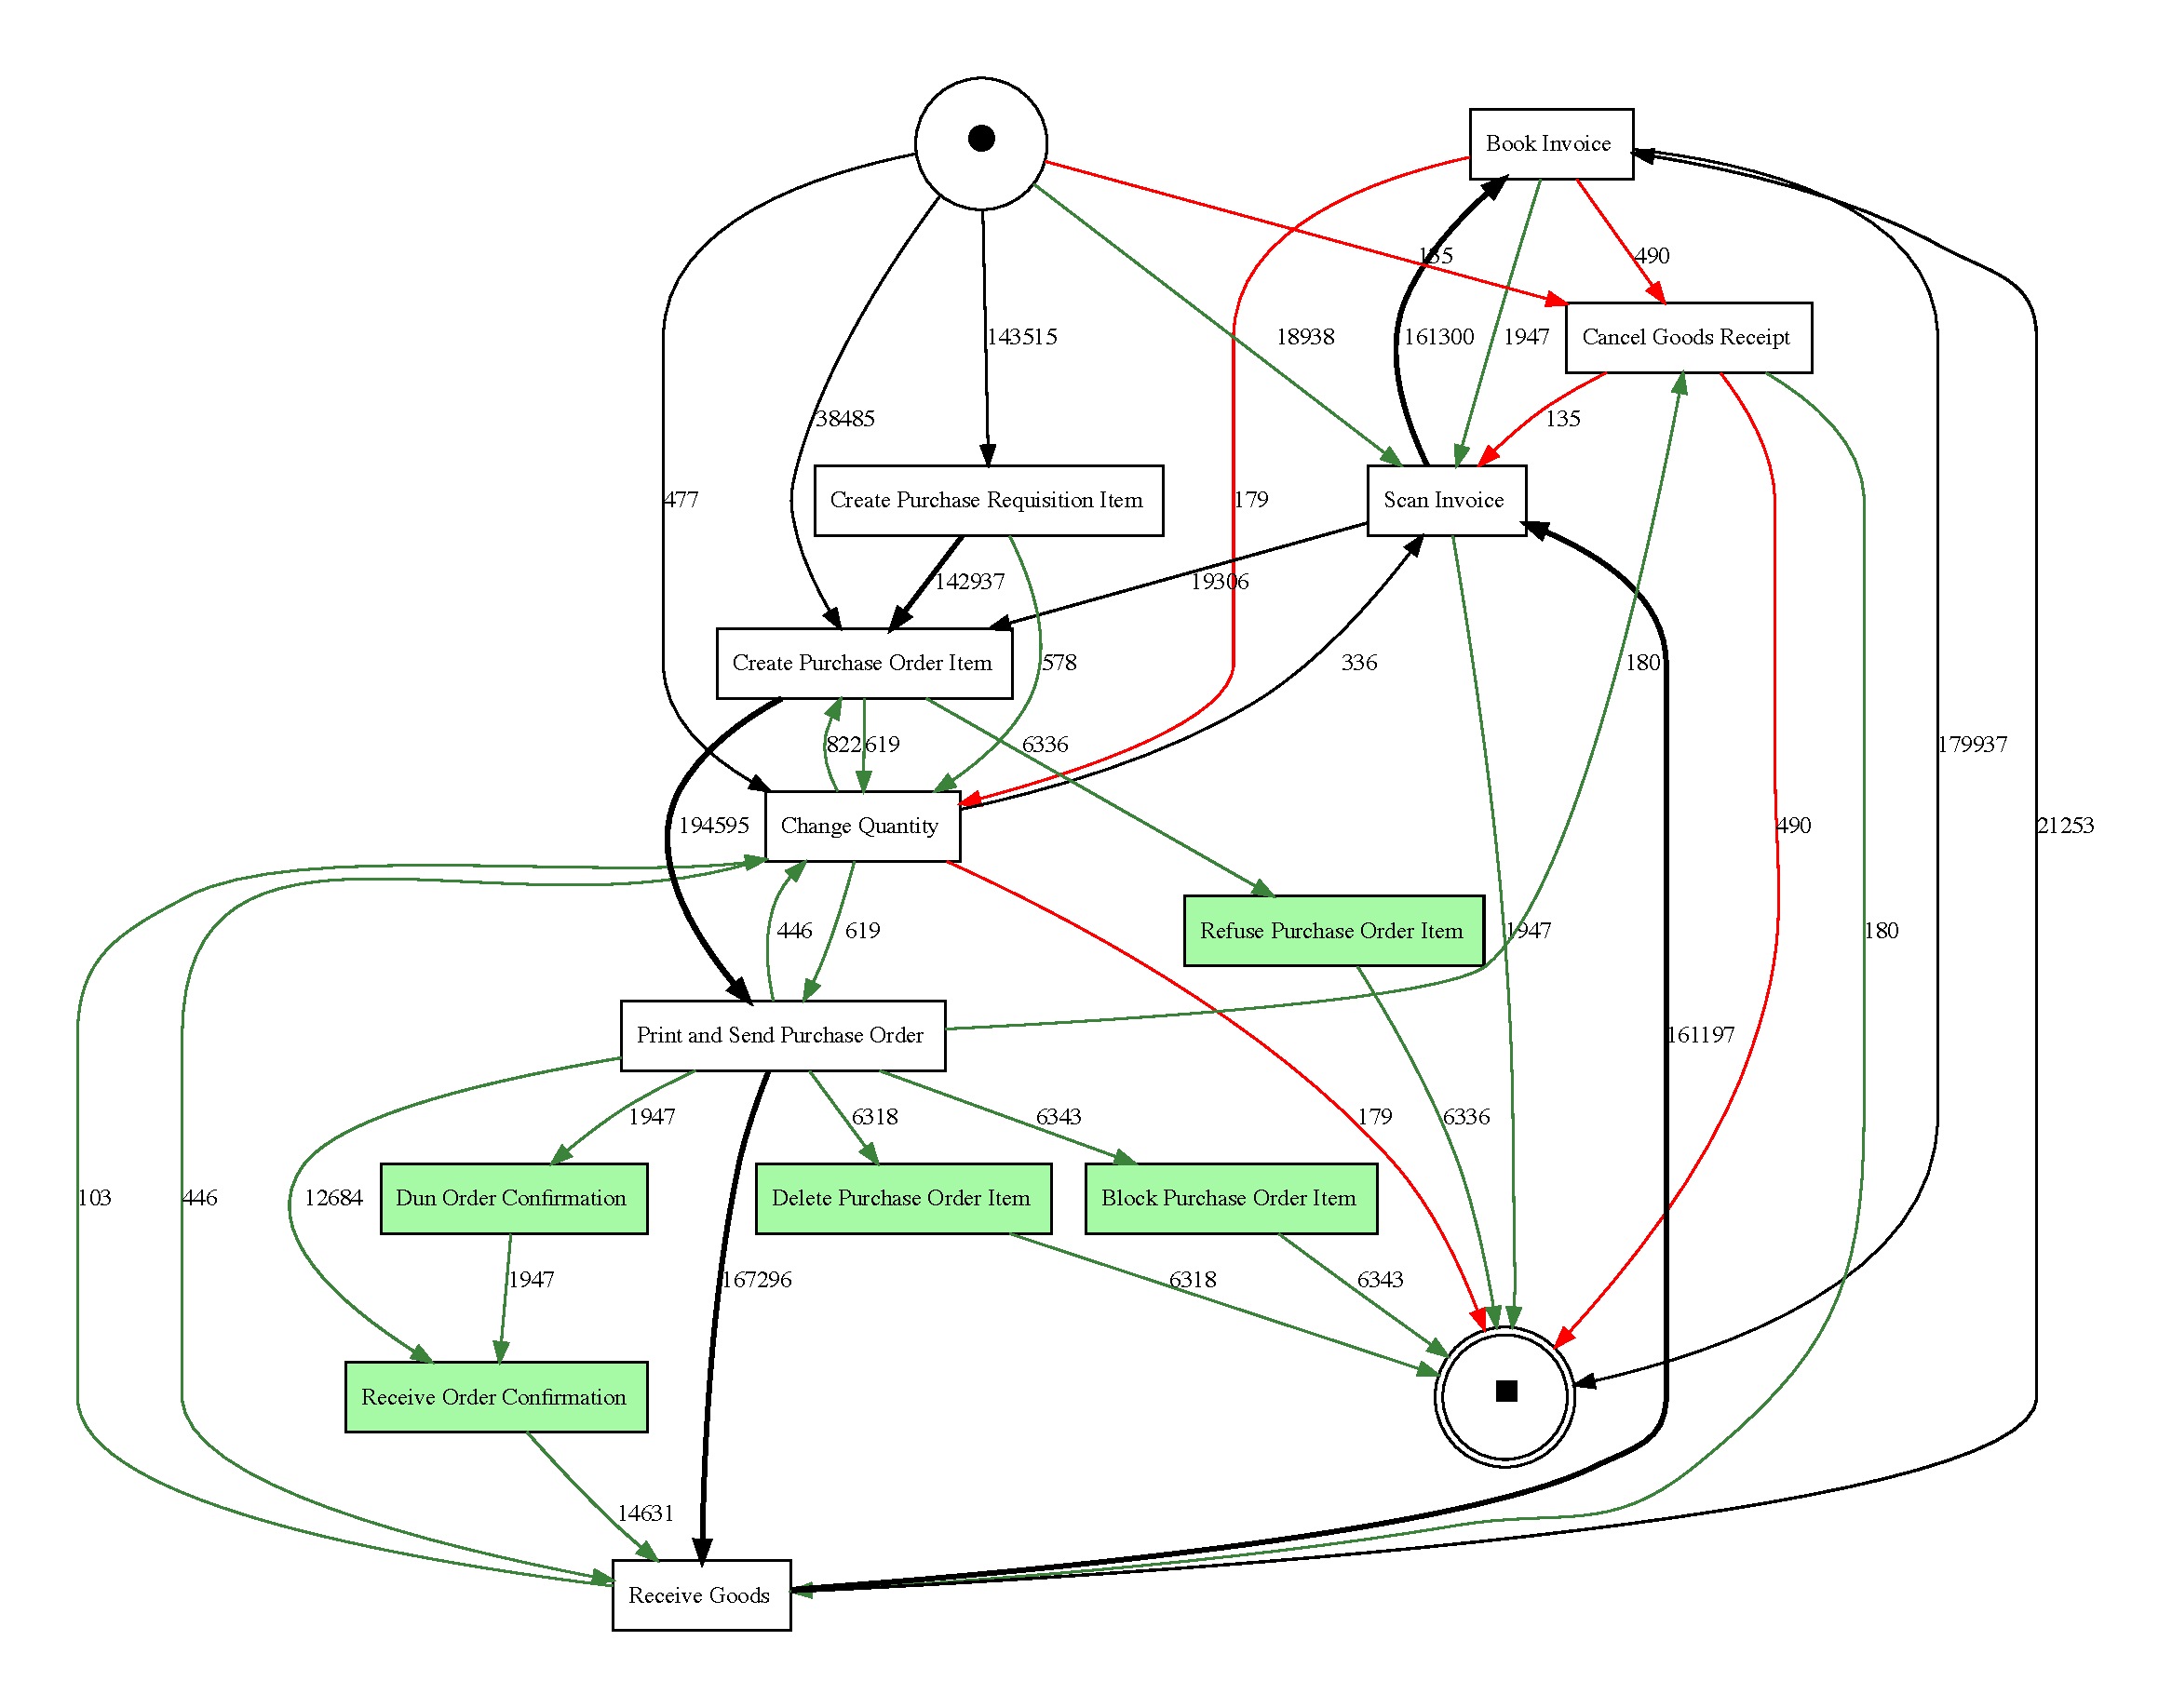
\includegraphics[width=\textwidth]{fig/ch3/bpi-eg-vc}
	\caption{The DFG highlighting the root causes of performance differences between the process variants. The set $\mathcal{G}reen$ constitutes $\mathcal{R}_0$, $\mathcal{R}_1$ and $\mathcal{R}_2$, and the set $\mathcal{R}ed$ constitutes $\mathcal{R}_5$.}
	\label{fig3:bpi-eg-vc}
\end{figure}

\begin{figure}[h!]
	\centering
	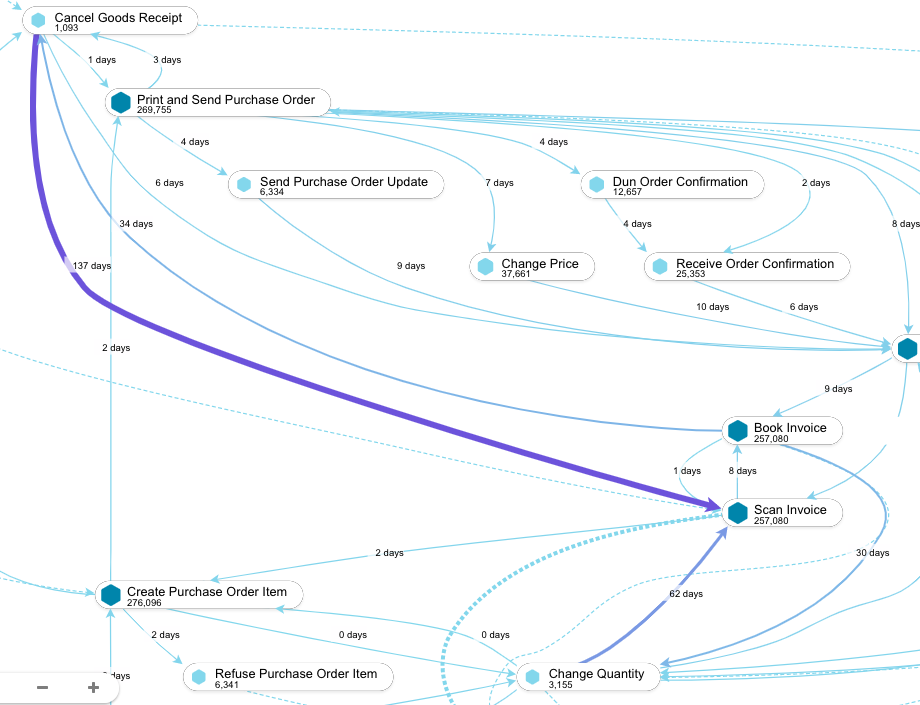
\includegraphics[width=\textwidth]{fig/ch3/bpi-eg-celonis}
	\caption{Screenshot of the DFG rendered by Celonis.}
	\label{fig3:bpi-eg-celonis}
\end{figure}

We compare our constructed DFG with the DFG generated by the Celonis application, noting that the Celonis DFG does not apply partial ranking to classify and colors the nodes and edges based on the performance classes. A screenshot of a portion of the Celonis DFG is displayed in Figure~\ref{fig3:bpi-eg-celonis}. In the Celonis DFG, the numbers displayed on the edges represent the median time between the start of two activities. Notably, there are significant time delays observed between the activities `Cancel Goods Receipt' to `Scan Invoice' (\textbf{e1}), `Change Quantity' to `Scan Invoice' (\textbf{e2}), and `Book Invoice' to `Change Quantity' (\textbf{e3}), indicating potential bottlenecks in the process flow. It is important to note that if a bottleneck occurs consistently across all process variants, it may not provide insights into the root cause of performance differences among the variants. However, when a bottleneck is present in some variants and not in others, it becomes a focal point for highlighting performance differences. While the Celonis DFG effectively captures these bottlenecks, it does not explicitly indicate whether these bottlenecks are the underlying causes of performance disparities among the variants. For example, in our DFG, the edge \textbf{e2} with a median time of 62 days is not highlighted in red as it appears in variants from both $\mathcal{G}reen$ and $\mathcal{R}ed$. Therefore, it is not inferred to directly contribute to the root cause of performance differences among the variants. However, the edge \textbf{e3}, with a median time of only 30 days, is marked in red in our DFG, suggesting it as an indicator of performance difference.

Thus, we remark that Celonis can benefit from incorporating partial ranking to provide additional perspectives within their DFG. This enhancement has the potential to offer valuable insights to their customers, aiding them in their decision-making processes.





\section{Summary}
\label{sec3:con}

 We considered the problem of ranking sets of noisy measurement data while accounting for ties. As soon as ties are allowed, more than one reasonable ranking became possible because of the non-transitive nature of the ties. For given sets of measurements and a  better-than relation that defines how two sets of measurements should be compared, we defined partial ranking to identify a set of reasonable rankings. We formalized and developed three different methodologies for partial ranking. Methodology~\ref{th:problem2} computes the partial ranking consisting of an arbitrary number of ranks. Methodology~\ref{th:problem3} takes the partial ranking computed by Methodology~\ref{th:problem2} as input and aims to reduce the number of ranks. This methodology identifies an alternate partial ranking and does not necessarily compute the minimum possible number of ranks. It is particularly useful in avoiding ties due to single variant mutually overlapping with more than two variants having well-separated IQIs. Finally, we presented Methodology~\ref{th:problem4} which computes the partial ranking with minimum possible number of ranks. An avenue for further extension of this research is the development of an efficient algorithm to systematically identify all possible partial rankings. 
 
%  when one wants to minimize the number of ranks but at the same time does not want the ranks of several variants whose IQIs are well separated to be tied because of a single mutually overlapping variant. 
% 
% (Sort-based), which employs a Bubble-sort based sorting procedure, can be used to search for alternative partial rankings by changing the input arrangements before sorting. Methodology~\ref{th:problem2} (Directed-graph-based) aims to identify a partial ranking with the maximum possible number of ranks, and Methodology~\ref{th:problem3} seeks to generate a partial ranking with fewer ranks, although not necessarily the minimum possible number. 

%a set of variants where each variant was characterized by a set of noisy measurement data. Given a better-than relation that defines how two sets of measurements should be compared, we developed methodologies of ranking sets of measurements while allowing for ties.
%
%given a set of algorithmic variants with each variant characterized by a set execution time measurements and a better-than relation that defines how two sets of measurements should be compared, we considered the problem of ranking those sets of measurements while allowing for ties. Since we allowed for ties, we found that more than one reasonable rankings became possible because of the non-transitive nature of the ties. We explored the ambiguities in the rankings, and conceptualized a set of reasonable rankings called partial rankings. We presented three different methodologies for partial ranking. Methodology~\ref{th:problemw} (Sort-based), employing a Bubble-sort based sorting procedure, can be used to search for alternative partial rankings by changing the input arrangements before sorting. While Methodology~\ref{th:problem2} (Directed-graph-based) aims to identify a partial ranking with the maximum possible number of ranks,  Methodology~\ref{th:problem3} seeks to generate a partial ranking with fewer ranks, although not necessarily the minimum possible number of ranks. 
%For our analysis, we summarized each set of measurement values as an interval number between two quantiles and employed a better-than relation that compares two sets of measurements based on their quantile limits. This approach is suitable, particularly in cases where data is limited or when acquiring measurement data is a costly endeavour. 

%We showcased the application of partial ranking by demonstrating how it aids in identifying the root causes behind performance differences among the variants, especially when dealing with noisy measurement data.
We then demonstrated the application of partial ranking in discerning observations that could facilitate in identifying the causes of performance differences among the variants. This discerning information can be used as ground truths to train models that can automatically differentiate between the variants, particularly in scenarios where performance measurements are not available. 

%By utilizing the samples of measurement values from different variants, we showed how the partial ranking methods can be applied to identify a subset of best variants and discern the distinguishing factors that contribute to their superior performance compared to variants from lower ranks. In the following chapter, we use this discerning information as ground truths to train models that guide in the selection of algorithmic variants, particularly in scenarios where the execution times are not measured.

\section*{Acknowledgments}

Financial support from the Deutsche Forschungsgemeinschaft (German Research Foundation) through grants GSC 111 and IRTG 2379 is gratefully acknowledged. 
%
%This section has a special environment:
%\begin{verbatim}
%  \begin{acks}
%  ...
%  \end{acks}
%\end{verbatim}
%so that the information contained therein can be more easily collected
%during the article metadata extraction phase, and to ensure
%consistency in the spelling of the section heading.
%
%Authors should not prepare this section as a numbered or unnumbered {\verb|\section|}; please use the ``{\verb|acks|}'' environment.

%\section{Appendices}
%
%If your work needs an appendix, add it before the
%``\verb|\end{document}|'' command at the conclusion of your source
%document.



%%
%% The next two lines define the bibliography style to be used, and
%% the bibliography file.
\bibliographystyle{ACM-Reference-Format}
\bibliography{general,mypub,ranking}

%%
%% If your work has an appendix, this is the place to put it.


\end{document}
\endinput
%%
%% End of file `sample-manuscript.tex'.
